%==============================================================================
% tento soubor pouzijte jako zaklad
% this file should be used as a base for the thesis
% Autoři / Authors: 2008 Michal Bidlo, 2019 Jaroslav Dytrych
% Kontakt pro dotazy a připomínky: sablona@fit.vutbr.cz
% Contact for questions and comments: sablona@fit.vutbr.cz
%==============================================================================
% kodovani: UTF-8 (zmena prikazem iconv, recode nebo cstocs)
% encoding: UTF-8 (you can change it by command iconv, recode or cstocs)
%------------------------------------------------------------------------------
% zpracování / processing: make, make pdf, make clean
%==============================================================================
% Soubory, které je nutné upravit nebo smazat: / Files which have to be edited or deleted:
%   xslade21-Klasifikace-hudebnich-souboru-20-literatura-bibliography.bib - literatura / bibliography
%   xslade21-Klasifikace-hudebnich-souboru-01-kapitoly-chapters.tex - obsah práce / the thesis content
%   xslade21-Klasifikace-hudebnich-souboru-01-kapitoly-chapters-en.tex - obsah práce v angličtině / the thesis content in English
%   xslade21-Klasifikace-hudebnich-souboru-30-prilohy-appendices.tex - přílohy / appendices
%   xslade21-Klasifikace-hudebnich-souboru-30-prilohy-appendices-en.tex - přílohy v angličtině / appendices in English
%==============================================================================
\documentclass[zadani]{fitthesis} % bez zadání - pro začátek práce, aby nebyl problém s překladem
%\documentclass[english]{fitthesis} % without assignment - for the work start to avoid compilation problem
%\documentclass[zadani]{fitthesis} % odevzdani do wisu a/nebo tisk s barevnými odkazy - odkazy jsou barevné
%\documentclass[english,zadani]{fitthesis} % for submission to the IS FIT and/or print with color links - links are color
%\documentclass[zadani,print]{fitthesis} % pro černobílý tisk - odkazy jsou černé
%\documentclass[english,zadani,print]{fitthesis} % for the black and white print - links are black
%\documentclass[zadani,cprint]{fitthesis} % pro barevný tisk - odkazy jsou černé, znak VUT barevný
%\documentclass[english,zadani,cprint]{fitthesis} % for the print - links are black, logo is color
% * Je-li práce psaná v anglickém jazyce, je zapotřebí u třídy použít 
%   parametr english následovně:
%   If thesis is written in English, it is necessary to use 
%   parameter english as follows:
%      \documentclass[english]{fitthesis}
% * Je-li práce psaná ve slovenském jazyce, je zapotřebí u třídy použít 
%   parametr slovak následovně:
%   If the work is written in the Slovak language, it is necessary 
%   to use parameter slovak as follows:
%      \documentclass[slovak]{fitthesis}
% * Je-li práce psaná v anglickém jazyce se slovenským abstraktem apod., 
%   je zapotřebí u třídy použít parametry english a enslovak následovně:
%   If the work is written in English with the Slovak abstract, etc., 
%   it is necessary to use parameters english and enslovak as follows:
%      \documentclass[english,enslovak]{fitthesis}

% Základní balíčky jsou dole v souboru šablony fitthesis.cls
% Basic packages are at the bottom of template file fitthesis.cls
% zde můžeme vložit vlastní balíčky / you can place own packages here
\usepackage{dirtree}
\usepackage{algorithm}
\usepackage{algpseudocode}

% Kompilace po částech (rychlejší, ale v náhledu nemusí být vše aktuální)
% Compilation piecewise (faster, but not all parts in preview will be up-to-date)
% \usepackage{subfiles}

% Nastavení cesty k obrázkům
% Setting of a path to the pictures
%\graphicspath{{obrazky-figures/}{./obrazky-figures/}}
%\graphicspath{{obrazky-figures/}{../obrazky-figures/}}

%---rm---------------
\renewcommand{\rmdefault}{lmr}%zavede Latin Modern Roman jako rm / set Latin Modern Roman as rm
%---sf---------------
\renewcommand{\sfdefault}{qhv}%zavede TeX Gyre Heros jako sf
%---tt------------
\renewcommand{\ttdefault}{lmtt}% zavede Latin Modern tt jako tt

% vypne funkci šablony, která automaticky nahrazuje uvozovky,
% aby nebyly prováděny nevhodné náhrady v popisech API apod.
% disables function of the template which replaces quotation marks
% to avoid unnecessary replacements in the API descriptions etc.
\csdoublequotesoff


\usepackage{subcaption}
\usepackage{url}


% =======================================================================
% balíček "hyperref" vytváří klikací odkazy v pdf, pokud tedy použijeme pdflatex
% problém je, že balíček hyperref musí být uveden jako poslední, takže nemůže
% být v šabloně
% "hyperref" package create clickable links in pdf if you are using pdflatex.
% Problem is that this package have to be introduced as the last one so it 
% can not be placed in the template file.
\ifWis
\ifx\pdfoutput\undefined % nejedeme pod pdflatexem / we are not using pdflatex
\else
  \usepackage{color}
  \usepackage[unicode,colorlinks,hyperindex,plainpages=false,pdftex]{hyperref}
  \definecolor{hrcolor-ref}{RGB}{223,52,30}
  \definecolor{hrcolor-cite}{HTML}{2F8F00}
  \definecolor{hrcolor-urls}{HTML}{092EAB}
  \hypersetup{
	linkcolor=hrcolor-ref,
	citecolor=hrcolor-cite,
	filecolor=magenta,
	urlcolor=hrcolor-urls
  }
  \def\pdfBorderAttrs{/Border [0 0 0] }  % bez okrajů kolem odkazů / without margins around links
  \pdfcompresslevel=9
\fi
\else % pro tisk budou odkazy, na které se dá klikat, černé / for the print clickable links will be black
\ifx\pdfoutput\undefined % nejedeme pod pdflatexem / we are not using pdflatex
\else
  \usepackage{color}
  \usepackage[unicode,colorlinks,hyperindex,plainpages=false,pdftex,urlcolor=black,linkcolor=black,citecolor=black]{hyperref}
  \definecolor{links}{rgb}{0,0,0}
  \definecolor{anchors}{rgb}{0,0,0}
  \def\AnchorColor{anchors}
  \def\LinkColor{links}
  \def\pdfBorderAttrs{/Border [0 0 0] } % bez okrajů kolem odkazů / without margins around links
  \pdfcompresslevel=9
\fi
\fi
% Řešení problému, kdy klikací odkazy na obrázky vedou za obrázek
% This solves the problems with links which leads after the picture
\usepackage[all]{hypcap}

% Informace o práci/projektu / Information about the thesis
%---------------------------------------------------------------------------
\projectinfo{
  %Prace / Thesis
  project={BP},            %typ práce BP/SP/DP/DR  / thesis type (SP = term project)
  year={2020},             % rok odevzdání / year of submission
  date=\today,             % datum odevzdání / submission date
  %Nazev prace / thesis title
  title.cs={Klasifikace hudebních souborů \\ pomocí strojového učení},  % název práce v češtině či slovenštině (dle zadání) / thesis title in czech language (according to assignment)
  title.en={Classification of Music Files Using Machine Learning}, % název práce v angličtině / thesis title in english
  %title.length={14.5cm}, % nastavení délky bloku s titulkem pro úpravu zalomení řádku (lze definovat zde nebo níže) / setting the length of a block with a thesis title for adjusting a line break (can be defined here or below)
  %sectitle.length={14.5cm}, % nastavení délky bloku s druhým titulkem pro úpravu zalomení řádku (lze definovat zde nebo níže) / setting the length of a block with a second thesis title for adjusting a line break (can be defined here or below)
  %Autor / Author
  author.name={Matyáš},   % jméno autora / author name
  author.surname={Sládek},   % příjmení autora / author surname 
  %author.title.p={Bc.}, % titul před jménem (nepovinné) / title before the name (optional)
  %author.title.a={Ph.D.}, % titul za jménem (nepovinné) / title after the name (optional)
  %Ustav / Department
  department={UITS}, % doplňte příslušnou zkratku dle ústavu na zadání: UPSY/UIFS/UITS/UPGM / fill in appropriate abbreviation of the department according to assignment: UPSY/UIFS/UITS/UPGM
  % Školitel / supervisor
  supervisor.name={Vladimír},   % jméno školitele / supervisor name 
  supervisor.surname={Janoušek},   % příjmení školitele / supervisor surname
  supervisor.title.p={Doc. Ing.},   %titul před jménem (nepovinné) / title before the name (optional)
  supervisor.title.a={Ph.D.},    %titul za jménem (nepovinné) / title after the name (optional)
  % Klíčová slova / keywords
  keywords.cs={strojové učení, předzpracování dat, extrakce atributů, selekce atributů, optimalizace parametrů, klasifikace}, % klíčová slova v českém či slovenském jazyce / keywords in czech or slovak language
  keywords.en={machine learning, data preprocessing, feature extraction, feature selection, parameter optimization, classification}, % klíčová slova v anglickém jazyce / keywords in english
  %keywords.en={Here, individual keywords separated by commas will be written in English.},
  % Abstrakt / Abstract
  abstract.cs={Tato práce se zabývá klasifikací hudebních souborů pomocí algoritmů strojového učení. V práci bylo porovnáno sedm klasifikačních algoritmů z hlediska úspěšnosti klasifikace a rychlosti zpracování na třech datových sadách. Využity byly dvě metody pro extrakci atributů, dvě metody pro selekci atributů a dvě metody optimalizace parametrů. Nejvíce se osvědčil model \textit{XGBClassifier}, který dosáhl úspěšnosti klasifikace 87.56 \% na datové sadě \uv{Extended Ballroom Dataset}, 64.56 \% na datové sadě \uv{FMA: A~Dataset For Music Analysis} a 83.50 \% na datové sadě \uv{GTZAN}. Tento model může být využit při tvorbě seznamů skladeb či kategorizaci hudební databáze.}, % abstrakt v českém či slovenském jazyce / abstract in czech or slovak language
  abstract.en={This thesis is focused on classification of music files using machine learning algorithms. Seven classifiers were compared in this thesis, based on classification accuracy and speed. Two feature extraction methods, two feature selection methods and two parameter optimization methods were used. The best classifier proved to be \textit{XGBClassifier}, which had reached accuracy of 87.56 \% on dataset \uv{Extended Ballroom Dataset}, 64.56 \% on dataset \uv{FMA: A~Dataset For Music Analysis} and 83.50 \% on dataset \uv{GTZAN}. This model could be used for playlist creation or music database categorization.}, % abstrakt v anglickém jazyce / abstract in english
  %abstract.en={An abstract of the work in English will be written in this paragraph.},
  % Prohlášení (u anglicky psané práce anglicky, u slovensky psané práce slovensky) / Declaration (for thesis in english should be in english)
  declaration={Prohlašuji, že jsem tuto bakalářskou práci vypracoval samostatně pod vedením pana Doc. Ing. Vladimíra Janouška Ph.D. Uvedl jsem všechny literární prameny, publikace a další zdroje, ze kterých jsem čerpal.},
  %declaration={I hereby declare that this Bachelor's thesis was prepared as an original work by the author under the supervision of Mr. X
% The supplementary information was provided by Mr. Y
% I have listed all the literary sources, publications and other sources, which were used during the preparation of this thesis.},
  % Poděkování (nepovinné, nejlépe v jazyce práce) / Acknowledgement (optional, ideally in the language of the thesis)
  acknowledgment={Rád bych poděkoval panu Doc. Ing. Vladimíru Janouškovi Ph.D. za skvělé vedení a cenné rady, které mi poskytl při tvorbě této bakalářské práce.},
  %acknowledgment={Here it is possible to express thanks to the supervisor and to the people which provided professional help
%(external submitter, consultant, etc.).},
  % Rozšířený abstrakt (cca 3 normostrany) - lze definovat zde nebo níže / Extended abstract (approximately 3 standard pages) - can be defined here or below
  %extendedabstract={Do tohoto odstavce bude zapsán rozšířený výtah (abstrakt) práce v českém (slovenském) jazyce.},
  %faculty={FIT}, % FIT/FEKT/FSI/FA/FCH/FP/FAST/FAVU/USI/DEF
  faculty.cs={Fakulta informačních technologií}, % Fakulta v češtině - pro využití této položky výše zvolte fakultu DEF / Faculty in Czech - for use of this entry select DEF above
  faculty.en={Faculty of Information Technology}, % Fakulta v angličtině - pro využití této položky výše zvolte fakultu DEF / Faculty in English - for use of this entry select DEF above
  department.cs={Ústav matematiky}, % Ústav v češtině - pro využití této položky výše zvolte ústav DEF nebo jej zakomentujte / Department in Czech - for use of this entry select DEF above or comment it out
  department.en={Institute of Mathematics} % Ústav v angličtině - pro využití této položky výše zvolte ústav DEF nebo jej zakomentujte / Department in English - for use of this entry select DEF above or comment it out
}

% Rozšířený abstrakt (cca 3 normostrany) - lze definovat zde nebo výše / Extended abstract (approximately 3 standard pages) - can be defined here or above
%\extendedabstract{Do tohoto odstavce bude zapsán výtah (abstrakt) práce v českém (slovenském) jazyce.}

% nastavení délky bloku s titulkem pro úpravu zalomení řádku - lze definovat zde nebo výše / setting the length of a block with a thesis title for adjusting a line break - can be defined here or above
%\titlelength{14.5cm}
% nastavení délky bloku s druhým titulkem pro úpravu zalomení řádku - lze definovat zde nebo výše / setting the length of a block with a second thesis title for adjusting a line break - can be defined here or above
%\sectitlelength{14.5cm}

% řeší první/poslední řádek odstavce na předchozí/následující stránce
% solves first/last row of the paragraph on the previous/next page
\clubpenalty=10000
\widowpenalty=10000

% checklist
\newlist{checklist}{itemize}{1}
\setlist[checklist]{label=$\square$}

\begin{document}
  % Vysazeni titulnich stran / Typesetting of the title pages
  % ----------------------------------------------
  \maketitle
  % Obsah
  % ----------------------------------------------
  \setlength{\parskip}{0pt}

  {\hypersetup{hidelinks}\tableofcontents}
  
  % Seznam obrazku a tabulek (pokud prace obsahuje velke mnozstvi obrazku, tak se to hodi)
  % List of figures and list of tables (if the thesis contains a lot of pictures, it is good)
  \ifczech
    \renewcommand\listfigurename{Seznam obrázků}
  \fi
  \ifslovak
    \renewcommand\listfigurename{Zoznam obrázkov}
  \fi
  % {\hypersetup{hidelinks}\listoffigures}
  
  \ifczech
    \renewcommand\listtablename{Seznam tabulek}
  \fi
  \ifslovak
    \renewcommand\listtablename{Zoznam tabuliek}
  \fi
  % {\hypersetup{hidelinks}\listoftables}

  \ifODSAZ
    \setlength{\parskip}{0.5\bigskipamount}
  \else
    \setlength{\parskip}{0pt}
  \fi

  % vynechani stranky v oboustrannem rezimu
  % Skip the page in the two-sided mode
  \iftwoside
    \cleardoublepage
  \fi

  % Text prace / Thesis text
  % ----------------------------------------------
  \ifenglish
    \input{xslade21-Klasifikace-hudebnich-souboru-01-kapitoly-chapters-en}
  \else
    %===============================================================================
% Autor: Matyáš Sládek
% Rok: 2020
%===============================================================================

\newcolumntype{Y}{>{\arraybackslash}X}
\hyphenation{GridSampler}
\hyphenation{TPESampler}
\hyphenation{LogisticRegression}
\hyphenation{KNeighborsClassifier}
\hyphenation{MLPClassifier}
\hyphenation{DecisionTreeClassifier}
\hyphenation{RandomForestClassifier}
\hyphenation{XGBClassifier}
\hyphenation{HPoptimise}
\hyphenation{MusicExtractor}

\chapter{Úvod}
\label{uvod}
Rozvoj informačních technologií umožnil uchovávat a šířit hudební skladby zcela novým způsobem. Lidé tak z~praktických důvodů postupně upouštěli od fyzických médií a shromažďovali skladby do hudebních databází v~digitální formě. Tyto databáze je vhodné přehledně organizovat, například rozdělením skladeb do kategorií na základě jejich hudebního obsahu. Tato kategorizace je velmi důležitá obzvláště z~pohledu tvorby takzvaných \uv{playlistů}, tedy seznamů skladeb s~podobným obsahem, se kterými se můžeme setkat například u~online streamovacích databází jako Spotify či Tidal.

Anotace obsahu hudebních souborů je v~dnešní době prováděna ručně. Tato práce se zabývá návrhem a implementací systému pro automatickou anotaci hudebních skladeb pomocí analýzy jejich obsahu.

V~kapitole~\ref{uvod_do_problematiky} jsou čtenáři přiblíženy základní informace nutné k~pochopení problematiky klasifikace digitálních hudebních souborů. V~úvodních podkapitolách jsou popsány některé ze základních veličin popisujících zvukové vlnění. Přiblíženy jsou také způsoby záznamu a uchování zvukových stop a některé z~pojmů hudební teorie. Závěr kapitoly se pak věnuje způsobům kategorizace hudebních databází a také použitým metodám a dosaženým výsledkům u~několika z~dostupných studií v~oboru klasifikace hudebních souborů.

Kapitola~\ref{predzpracovani_dat} přibližuje čtenáři vybrané způsoby předzpracování dat vhodné pro klasifikaci hudebních souborů. Popsány jsou metody extrakce vhodných atributů ze zvukových stop a také metody selekce nejvhodnějších z~těchto atributů pro efektivní zpracování klasifikačními algoritmy. Na konci kapitoly jsou popsány nejpoužívanější z~metod kódování a škálování dat.

Čtvrtá kapitola~\ref{klasifikacni_algoritmy} seznamuje čtenáře s~přístupy ke klasifikaci dat a také s~některými z~nejznámějších klasifikačních algoritmů. Zmíněny jsou pravděpodobnostní metody, rozhodovací stromy, metody učení založené na instancích, metody podpůrných vektorů a neuronové sítě. V~poslední podkapitole~\ref{ensemble_metody} této kapitoly jsou pak přiblíženy přístupy k~vytváření takzvaných \uv{ensemble metod}, což jsou metody kombinující několik klasifikátorů dohromady.

V~kapitole~\ref{navrh_a_implementace_systemu} jsou popsány některé z~volně dostupných datových sad, které lze pro trénování modelů využít. Dále jsou popsány využité způsoby předzpracování dat, zahrnující kódování a škálování dat, extrakci atributů a selekci atributů. Zmíněn je také výběr klasifikačních algoritmů a nakonec je popsán způsob optimalizace parametrů těchto algoritmů.

V~předposlední kapitole~\ref{klasifikace_a_zhodnoceni_vysledku} je pak vyhodnocena úspěšnost klasifikace na testovacích datech všech tří datových sad a v~závěrečné~\ref{zaver}. kapitole je pak shrnuta provedená práce a možnosti budoucího vývoje.

\chapter{Úvod do problematiky}
\label{uvod_do_problematiky}
Tato kapitola pojednává o~základních vlastnostech zvuku a způsobech jeho záznamu a uchování. Dále pak vysvětluje základní pojmy hudební teorie používané v~následujících kapitolách a přiblíženy jsou i způsoby kategorizace hudebních souborů na základě jejich obsahu. Nakonec je pak zmíněno několik z~dosavadních prací na téma klasifikace muziky pomocí strojového učení.

\section{Zvuk}
\label{zvuk}
Zvuk je možné popsat jako změnu tlaku v~závislosti na čase a šíří se jako mechanické vlnění (oscilace molekul) prostřednictvím elastického média, jako je plyn, kapalina, pevná látka nebo plazma. Ve všech těchto skupenstvích se zvuk šíří jako podélné (také longitudální či tlakové) vlnění, při kterém dochází k~oscilaci částic ve směru rovnoběžném se směrem šíření vlnění. V~pevném skupenství se však dle některých zdrojů může zvuk šířit i jako vlnění příčné, při kterém dochází k~oscilaci částic ve směru kolmém na směr šíření vlnění.\cite{leisure_2017}\cite{music_theory}

Zvukové vlny lze popsat pomocí následujících vlastností:

\begin{itemize}
    \item Perioda - udává délku trvání jednoho cyklu vlny. Její jednotkou je obvykle sekunda a značí se $T$.
    \item Frekvence - inverzní hodnota periody, udává počet cyklů za jednu sekundu. Její jednotkou je Hertz a značí se $f$.
    \item Amplituda - u~zvukových vln značí rozsah pohybu částic vůči jejich rovnovážné poloze.
    \item Fáze - udává pozici počátku cyklu vlny.
    \item Rychlost zvuku - udává rychlost pohybu zvukových vln v~médiu, měří se obvykle v~metrech za sekundu a značí se $c$.
    \item Vlnová délka - udává vzdálenost, kterou vlna překoná za dobu jedné její periody, měří se obvykle v~metrech a značí se $\lambda$.
\end{itemize}

Znázornění zvukových vln je možné vidět v~obrázku~\ref{obr_sinusoidy}. Lidské ucho je citlivé na frekvence zvuků mezi přibližně 20 Hz a 20 kHz a změnu frekvence zvuků vnímá spíše logaritmicky, než lineárně. Stejně jako u~změn frekvence je lidské ucho citlivé i na změny tlaku logaritmicky, proto se používá pro vyjádření hlasitosti jednotka logaritmické stupnice decibel (dB). Decibel je bezrozměrná jednotka vyjadřující poměr dvou vstupních veličin. U~hlasitosti zvuků přenášených vzduchem se jako referenční vstupní hodnota používá nejnižší lidmi slyšitelná změna tlaku vzduchu.\cite{music_theory}\cite{db}

\begin{figure*}[h]
    \centering
    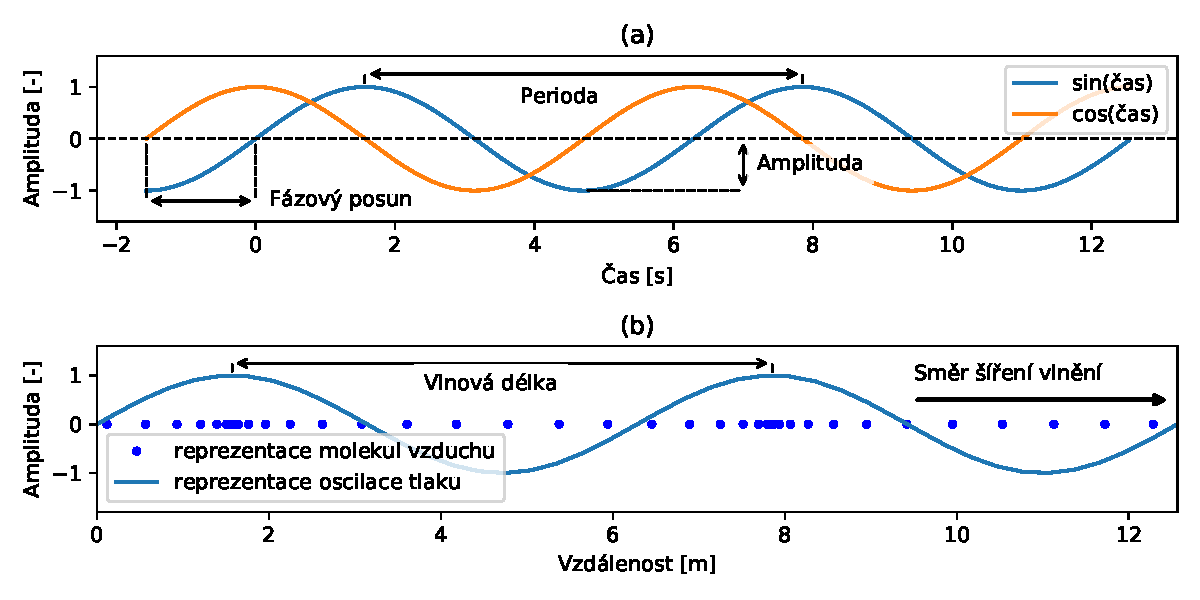
\includegraphics[width=\textwidth]{obrazky/sinusoidy.pdf}
    \caption{\textbf{Grafy zvukových vln.} (a) Graf funkcí sinus a cosinus. Z~grafu je patrné, že funkce kosinus je fázově posunutou funkcí sínus. (b) Ukázka podélného vlnění. Částice oscilující ve směru rovnoběžném se směrem šíření vlnění tvoří místa s~vyšší koncentrací (vyšší tlak) a nižší koncentrací (nižší tlak).}
    \label{obr_sinusoidy}
\end{figure*}

\section{Způsoby záznamu, uchování a reprodukce zvuku}
\label{zpusoby_zaznamu_uchovani_a_reprodukce_zvuku}
Záznam, uchování a reprodukci zvuku je možné rozdělit do dvou kategorií, a to analogové a digitální. Přes to, že dnes dominuje digitální způsob uchování dat, je stále možné setkat se s~nahrávkami analogovými, které jsou důležité i z~hlediska historického. V~následujících odstavcích je proto krátce zmíněna i tato varianta.\cite{dsp}\cite{aca}

Zvukové vlny je možné zaznamenat pomocí membrány mikrofonu, která snímá změny atmosferického tlaku a následně tyto pomocí mechanického či elektronického systému transformuje na analogový či digitální signál, který zapisuje na nějaké médium. Následná reprodukce je obráceným procesem záznamu, kde je signál z~média převeden pomocí membrány reproduktoru zpět na změny atmosferického tlaku.\cite{dsp}\cite{aca}

Analogový signál je spojitou funkcí spojitého času. Analogový signál může být uchován na médiích mechanických, jako je například vinylová deska, nebo magnetických jako je například magnetická páska. Přes to, že samotné zvukové vlny jsou analogovým signálem, v~dnešní době se ve většině případů z~praktických důvodů zvukové vlny uchovávají jako signál digitální.\cite{dsp}\cite{aca}

Digitální signál je oproti analogovému signálu funkcí diskrétního času, tedy je definován pouze v~diskrétních časových okamžicích. Tento signál je pak reprezentován posloupností funkčních hodnot. Převod analogového signálu na digitální probíhá pomocí periodického čtení hodnot analogového signálu a následného zapisování těchto hodnot na digitální médium, jako například pevný disk. Tento proces se nazývá vzorkování a frekvence, se kterou jsou hodnoty čteny a zapisovány se nazývá \textit{vzorkovací frekvence}. Obrázek~\ref{obr_vzorkovany_signal} obsahuje ukázku vzorkovaného signálu. Dle vzorkovacího teorému je pro bezchybné vzorkování signálu s~maximální frekvencí $f_{max}$ je nutné zvolit vzorkovací frekvenci $f_S$ tak, aby platil vztah

\begin{equation}
	f_{max} < f_S/2.
\end{equation}

\medskip

\noindent Pokud tento vztah dodržen není, dochází k~jevu zvanému \textit{aliasing}, kdy při vzorkování signálu dochází k~transformaci frekvencí na jiné.\cite{dsp}\cite{aca}

Následná reprodukce je dosažena převedením těchto hodnot zpět na analogový signál. O~tyto funkce se starají převodníky \textit{ADC (analog to digital converter)} a \textit{DAC (digital to analog converter)}. Uchování zvukových signálů v~digitální podobě má oproti podobě analogové řadu výhod, mezi které se řadí například možnost bezztrátového kopírování, menší velikost, vyšší odolnost vůči poškození, mnohem vyšší rychlost zápisu a čtení u~digitálních médií a další.\cite{dsp}

\begin{figure*}[h]
    \centering
    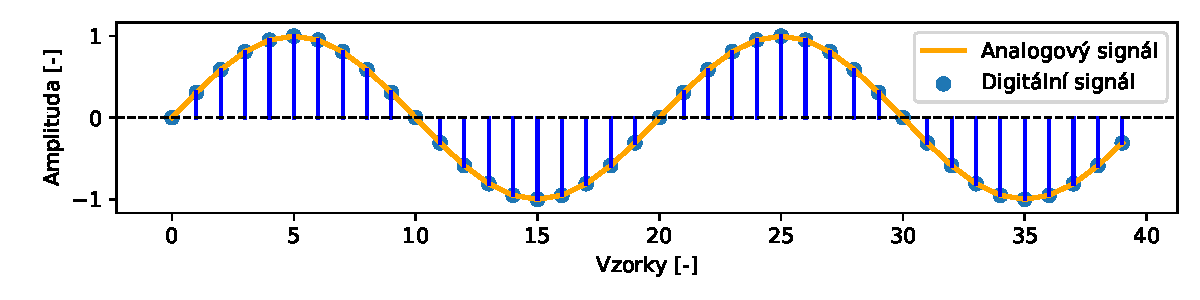
\includegraphics[width=\textwidth]{obrazky/vzorkovany_signal.pdf}
    \caption{\textbf{Graf reprezentací analogového a digitálního signálu.} Graf znázorňuje rozdíl mezi analogovým signálem sinusoidy s~frekvencí 400 Hz a její digitální reprezentací, kde při vzorkovací frekvenci 8000 Hz jednu periodu zachycuje 20 vzorků.}
    \label{obr_vzorkovany_signal}
\end{figure*}

\section{Hudba}
\label{hudba}
Jednoznačná definice hudby neexistuje, obecně se však dá říci, že se jedná o~uměleckou formu, jejíž médiem je soubor zvuků uspořádaný v~čase. Hudba má mnoho forem, může obsahovat zpěv, zvuky hudebních nástrojů, zvuky přírody a další. V~hudební teorii se zvuky dělí na hudební (tóny) a nehudební (hluky), kde tóny se vyznačují pravidelnou oscilací a hluky nepravidelnou oscilací zvukové vlny. Čistý tón obsahuje pouze jedinou frekvenci, avšak tóny produkované hudebními nástroji obsahují několik frekvencí. A~to základní frekvenci a frekvence harmonické, které jsou celočíselným násobkem frekvence základní. Jako výška tónu se v~hudební teorii označuje subjektivní vnímání jeho frekvence. Tóny produkují například strunné či dechové nástroje, zatím co hluky produkují převážně nástroje perkusní. V~hudební teorii se hudba nejčastěji popisuje pomocí rytmu, melodie, harmonie, barvy a textury, které jsou popsány v~následujícím seznamu.\cite{music_theory}\cite{MIR}

\begin{itemize}
    \item Rytmus popisuje rozložení zvuků v~čase. 
    \item Melodie značí posloupnost několika tónů po sobě.
    \item Harmonie označuje několik tónů různé výšky ve stejném okamžiku.
    \item Barva popisuje všechny vlastnosti zvuku mimo výšku, hlasitost a dobu trvání, jako například poměr amplitud frekvencí u~tónu.
    \item Textura popisuje komplexitu hudby, tedy kolik melodií, zvůků, nástrojů a dalších obsahuje v~daném časovém okamžiku.
\end{itemize}

V~hudební teorii je také možné se setkat s~pojmy jako stupnice, kde u~západní muziky se používá stupnice diatonická, která vychází ze stupnice chromatické. \textit{Chromatická stupnice} obsahuje dvanáct tónů v~jedné oktávě, jedná se tedy o~stupnici dvanáctitónovou. Oproti tomu \textit{diatonická stupnice} je sedmitónová, tedy obsahuje pouze vybraných sedm z~dvanácti těchto tónů. Kterých sedm tónů diatonická stupnice obsahuje, určuje takzvaná \textit{tónina}.\cite{MIR}

\section{Kategorizace hudebních skladeb}
\label{kategorizace_hudebnich_skladeb}
Nedílnou součástí organizace hudební databáze je rozdělení jejího obsahu do kategorií, tedy shlukování skladeb na základě určitých společných vlastností. Takováto kategorizace je vhodná hned z~několika důvodů, umožňuje uživatelům snadnější orientaci v~databázi, snadnější vyhledání podobných skladeb, případně umožňuje databázi vizualizovat. Uspořádání hudebních souborů do kategorií s~sebou však nese mnoho úskalí. Nejprve je potřeba určit, na základě jakých vlastností je vhodné skladby kategorizovat. Skladby je možné rozdělit do kategorií například podle roku vydání, či podle jejich autora, tyto kategorie nám však o~samotné hudební estetice skladby mnoho neřeknou. Z~toho důvodu lidé začali přicházet s~dalšími kategoriemi, zakládajících se na obsahu skladeb, tedy pocitu z~poslechu, použití určitých hudebních nástrojů, tempu a tak dále. Příkladem takovýchto kategorií mohou být například hudební žánry.

Hudební žánr je dnes nejpoužívanější formou popisu hudební estetiky muziky. Lze jej popsat jako druh muziky dodržující určitá pravidla, přijímaný nějakou komunitou. Mezi vlastnosti charakterizující hudební žánry patří tempo, použité hudební nástroje, popularita muziky, regionální výskyt muziky a spousta dalších. Hudební žánr nemá žádnou formální definici a každý jej tak vnímá do jisté míry subjektivně. Z~tohoto důvodu u~spousty skladeb není možné jednoznačně určit, pod jaký hudební žánr spadá a často se dnes setkáváme s~případy, kdy je jedna skladba označena hned několika žánry. Hudebních žánrů jsou v~dnešní době tisíce, avšak spousta z~nich je považována za \uv{podžánry} žánrů obecnějších. Například žánry Techno, Trance a House spadají pod žánr Dance. Hudební žánry vznikají zároveň s~nově vznikajícími formami a styly muziky, nebo kvůli potřebě jejich přesnější klasifikace.\cite{genre}\cite{aca}

Dalším možným kritériem pro klasifikaci jsou emoce, které skladby při poslechu evokují. Nejvíce zjevné, jak hudba evokuje určité emoce může být například ze zvukových stop k~filmům, které významným způsobem dokreslují atmosféru scény. Tento způsob klasifikace je ale opět do značné míry subjektivní a také je propojen s~žánry. Důležitými parametry pro tento způsob klasifikace jsou zejména tempo a tónina.\cite{5202572}\cite{aca}

Další množinou kategorií mohou být taneční styly. Tento způsob klasifikace je vhodné využít zejména u~databází určených pro diskotéky nebo taneční soutěže. U~klasických tanců je nejvíce směrodatný rytmus, u~modernějších tanců rytmus nemusí hrát roli a jediným parametrem pro klasifikaci pak zůstává tempo.

\section{Metody automatické klasifikace hudebních souborů}
\label{metody_automaticke_klasifikace_hudebnich_skladeb}
Automatické klasifikaci a doporučování podobné muziky je se stále rychleji narůstajícím počtem skladeb věnováno čím dál více pozornosti. V~dostupných studiích zabývajících se touto problematikou je možné narazit převážně na dva přístupy, prvním z~nich je klasifikace na základě nízkoúrovňových charakteristických dat získaných algoritmicky ze zvukové stopy a druhým je klasifikace na základě vysokoúrovňových charakteristických dat vytvořených lidmi. Oba tyto přístupy mají své výhody i nevýhody a u~každého z~nich byla demonstrována řada metod dosahujících různě přesných výsledků. Jelikož klasifikace na základě popisných vlastností vytvořenými lidmi je mimo rozsah této práce, tento přístup dále zmíněn není.

%\subsection*{Klasifikace muziky podle textových řetězců}
%\label{klasifikace_muziky_podle_textovych_retezcu}
%Klasifikace muziky podle textových řetězců probíhá pomocí vyhledání a zpracování společných výskytů textových řetězců, které se nějakým způsobem pojí s~danou skladbou. Příkladem takového textového řetězce může být slovo v~článku či sociální tag. Pokud se například v~jednom článku vyskytuje jméno hledaného interpreta a název určitého žánru, je zde šance, že díla daného interpreta spadají pod daný žánr. Stejně tak pokud nalezneme v~článku na webových stránkách jména dvou interpretů, je zde šance, že spolu tito interpreti sdílejí určité charakteristiky. Tato šance narůstá s~počtem těchto nalezených společných výskytů v~článku, o~to více pak v~případě nalezení ve více článcích.

%Tento způsob hledání analogií mezi skladbami či interprety a žánry má oproti klasifikaci podle obsahu audio stopy výhodu primárně v~tom, že není nutné provádět výpočetně náročné operace extrakce charakterizujících vlastností ze zvukové stopy a že zvukovou stopu vůbec nemusíme mít k~dispozici. Nevýhodou je závislost na datech vytvořených lidmi a jejich dostupnosti, v~některých případech pak i obtížná filtrace irelevantních dat. Dalším nedostatkem je nutnost mít k~dispozici název skladby a jméno autora. I~přes tyto nedostatky ale byly pomocí této metody dosaženy uspokojivé výsledky.\cite{5662276}\cite{Schedl05aweb-based}\cite{Knees04artistclassification}

\subsection*{Klasifikace muziky podle obsahu audio stopy}
\label{klasifikace_muziky_podle_obsahu_audio_stopy}
S~klasifikací podle obsahu audio stopy se v~dostupných studiích můžeme setkat častěji. Jde o~způsob klasifikace na základě informací získaných ze samotné zvukové stopy, které jsou následně předány ke zpracování klasifikačním algoritmům. Jelikož tento přístup pracuje pouze se samotnou zvukovou stopou, jednou z~jeho výhod je nezávislost na datech vytvořených lidmi. Mezi jeho nevýhody však patří nutnost provádět výpočetně náročné operace extrakce směrodatných informací ze zvukové stopy a trénování klasifikačních algoritmů. Dále je pak potřeba mít k~dispozici dostatečně obsáhlou datovou sadu, na které je možné klasifikátory natrénovat. V~následujících odstavcích jsou zmíněny a krátce popsány dostupné výzkumy zabývající se tímto způsobem klasifikace.

Jednu z~prvních prací na toto téma publikovali roku 2002 Tzanetakis a Cook. Ve své práci navrhli způsob klasifikace pomocí třech sad nízkoúrovňových atributů popisujících určitou vlastnost zvukové stopy. První sada obsahovala atributy popisující barvu zvuku, druhá rytmus a třetí výšku a tóninu. Tyto sady byly zpracovány pomocí Gaussova klasifikátoru, Gaussova smíšeného modelu a metody K-nejbližších sousedů. K~vyhodnocení byly použity tři datové sady dohromady obsahující dvacet žánrů, kde každý žánr byl reprezentován stem třiceti sekundových úseků skladeb. Výsledky klasifikace je možné vidět v~následujícím seznamu.\cite{1021072}

\begin{itemize}
\item Žánry: rozdělení do 10 skupin: 61 \%
\item Classical: rozdělení do 4 skupin: 85 \%
\item Jazz: rozdělení do 6 skupin: 67 \%
\end{itemize}

Gwardys a Grzywczak ve své práci využili pro klasifikaci výhradně spektrogram, čímž problém klasifikace zvukové stopy transformovali na problém klasifikace obrazu. Ke klasifikaci byly využity tři formy spektrogramu, a to původní obecný spektrogram, harmonický spektrogram a perkusní spektrogram. Pro klasifikaci byly využity konvoluční neuronové sítě. Nejlepších výsledků bylo dosaženo kombinací všech tří spektrogramů, kde pro každý z~nich byl zvlášť natrénován jeden klasifikátor a výsledky všech byly vyhodnoceny pomocí metody podpůrných vektorů. Tímto způsobem bylo dosaženo 78\% úspěšnosti při klasifikaci sta skladeb do desíti žánrů.\cite{DeepImageFeaturesinMusicInformationRetrieval}

Práce Murauera a Spechta porovnává více způsobů klasifikace. Jedním z~nich je klasifikace pomocí konvolučních neuronových sítí pracujících se spektrogramem, druhým je klasifikace pomocí algoritmů rozhodovacích stromů, posilování gradientu a hlubokých neuronových sítí pracujících s~numerickými parametry. Výsledky experimentů této práce naznačují, že pomocí klasifikátoru posilování gradientu XGBoost je možné dosáhnout ještě přesnějších výsledků, než pomocí neuronových sítí. A~to jak konvolučních pracujících se spektrogramem, tak hlubokých pracujících s~numerickými parametry. Jak však autoři sami zmiňují, tyto výsledky mohly být ovlivněny nedostatkem prostředků pro kvalitnější implementaci neuronových sítí.\cite{Murauer:2018:DMG:3184558.3191822}

Kaur a Kumar vybrali pro klasifikaci čtyři nízkoúrovňové vlastnosti, které na základě svého průzkumu vyhodnotili jako nejvíce přínosné. Byly to Mel-frekvenční kepstrální koeficienty, spektrální klesání, počet průchodů nulou a spektrální tok. Pro klasifikaci využili Gaussova smíšeného modelu a pro vyhodnocení výsledků využili čtyř datových sad, kde u~každé z~nich jejich způsob klasifikace dosáhl přibližně 70\% úspěšnosti.\cite{8365395}

S~klasifikací do žánrů se můžeme ve výzkumech komunity \textit{získávání hudebních informací (music information retrieval, MIR)} setkat nejčastěji, v~některých případech je ale možné se setkat i s~klasifikací do jiných kategorií, jako například emocí. Tento způsob zvolili ve své práci Lin, Yang, Chen, Liao a Ho, kde pro klasifikaci emocí nejprve využili klasifikace žánrů, neboť žánr je dle výsledků jejich experimentů s~emocemi do značné míry propojen. Klasifikace tedy probíhala na dvou úrovních, kdy v~první úrovni byl klasifikován žánr a v~druhé emoce. Pro klasifikaci žánrů zvolili dva způsoby, a to klasifikaci jednoho žánru a klasifikaci více žánrů, kde pravděpodobnost náležitosti k~určitému žánru byla vyjádřena procentuálně. U~obou způsobů byly následně informace získané z~klasifikace žánrů použity pro klasifikaci emocí a pro porovnání byl demonstrován i klasifikátor pracující s~reálnými informacemi o~žánru získaných z~hudebních databází. Výsledky experimentů ukázaly, že klasifikace s~využitím procentuální náležitosti k~žánrům byla jednak přesnější než klasifikace s~využitím jednoho žánru, ale také, že její úspěšnost se blížila výsledkům klasifikace s~použitím reálných informací o~žánru.\cite{5202572}

\chapter{Předzpracovaní dat}
\label{predzpracovani_dat}
\textit{Předzpracování dat (data preprocessing)} je jedním z~nejdůležitějších kroků v~oboru strojového učení. Jedná se o~proces, při kterém se původní data transformují tak, aby je vybraný algoritmus byl schopný lépe interpretovat a dosáhl lepších výsledků. Předzpracování dat se skládá z~několika kroků, ne vždy je však nutné provést všechny. Jaké kroky je vhodné provést záleží na formě a velikosti dat původních a na použitém algoritmu. Prvním krokem obvykle bývá kontrola kvality dat. Tento krok zahrnuje ošetření chybějících hodnot buďto jejich doplněním či odstraněním příslušných položek a také odstranění duplikátních a chybných hodnot. V~následujících odstavcích jsou blíže rozebrány vhodné kroky předzpracování dat pro klasifikaci hudebních souborů.\cite{data_preprocessing}\cite{aca}

Přestože s~využitím neuronových sítí na neupravené zvukové stopě bylo dosaženo uspokojivých výsledků, pro většinu klasifikačních algoritmů je digitální reprezentace zvukové stopy příliš komplexní na to, aby ji byly shopny efektivně zpracovat. Je tedy nejprve nutné ji vhodně upravit. Tento proces se nazývá redukce dimenzionality či snížení počtu rozměrů a dá se rozdělit do dvou hlavních kategoríí. Extrakce atributů a selekce atributů. Atribut (vlastnost) je v~tomto kontextu hodnota určitým způsobem popisující původní objekt. Atributy se dělí na numerické a kategorické. Numerické atributy jsou takové, jejichž hodnoty jsou spojité nebo celočíselné. Tyto atributy nemají definovanou konečnou množinu hodnot. Mezi atributy numerické patří například tempo skladby. Atributy kategorické jsou takové, které mají předem definovanou konečnou množinu hodnot. Patří mezi ně například dominantní tónina skladby.\cite{MIR}\cite{8733572}\cite{aca}

\section{Extrakce atributů}
\label{extrakce_atributu}
Extrakci atributů je vhodné použít v~případě, kdy původní data jsou příliš rozsáhlá nebo obsahují redundantní či irelevantní hodnoty. Extrakce atributů si klade za cíl tato data transformovat pomocí různých funkcí na data nová, méně rozsáhlá, avšak se zachováním co největšího množství informací. Přístupů k~extrakci atributů existuje mnoho a vhodné způsoby závisí na konkrétní situaci. Existuje spousta algoritmů implementovaných pro tento účel, které jsou dostatečně obecné na to, aby se daly použít napříč řadou oborů. Mezi zmíněné metody patří například \textit{Analýza hlavních komponent (Principal component analysis, PCA)} či poměrně nová metoda \textit{Jednotná mnohočetná aproximace a projekce (Uniform manifold approximation and projection, UMAP)}.\cite{data_classification}\cite{lel2018umap}\cite{aca}

V~oboru získávání hudebních informací však existuje celá řada algoritmů vytvořených specificky za účelem extrakce vhodných atributů ze zvukové stopy. Tyto atributy je pak možné rozdělit do tříd například dle úrovně abstrakce na nízkoúrovňové a vysokoúrovňové sémantické atributy, dle časového rozsahu na okamžité, segmentové či globální, případně dle aspektů hudební teorie na atributy týkající se melodie, rytmu, harmonie a dalších. Označení proměnných v~rovnicích této kapitoly jsou uvedeny v~tabulce~\ref{oznaceni_v_rovnicich_extrakce}.\cite{MIR}\cite{aca}

\begin{table}[H]
	\vskip6pt
	\caption{\textbf{Označení využitá v~rovnicích podkapitoly extrakce atributů}}
    \vskip6pt
	\centering
    \begin{tabular}{c | l} 
        \textbf{Označení} & \textbf{Popis} \\ [0.5ex] 
        \hline\hline
        $x[n]$ & Hodnota amplitudy vzorku $n$\\
        \hline
        $N$ & Celkový počet vzorků signálu \\
        \hline
        $X[k]$ & Hodnota amplitudy frekvence $k$ \\
        \hline
        $K$ & Celkový počet frekvencí spektra\\
        \hline
        $r$ & Označení okna $r$ \\
        \hline
        $s$ & Označení filtračního pásma $s$ \\
        \hline\hline
    \end{tabular}
	\label{oznaceni_v_rovnicich_extrakce}
\end{table}

\subsection*{Časová a frekvenční oblast}
\label{casova_a_frekvencni_oblast}
Digitální reprezentace zvukové stopy je funkcí času a jedná se tedy o~reprezentaci v~časové oblasti. Tato reprezentace zvukové stopy je vhodná pro extrakci atributů týkajících se vývoje amplitudy zvukové vlny v~čase. Frekvenční spektrum signálu v~časové oblasti je pak reprezentací tohoto signálu ve frekvenční oblasti, tedy je funkcí frekvence. Taková reprezentace je pak vhodná k~extrakci atributů týkajících se zastoupení jednotlivých frekvencí ve zvukové vlně. Zobrazení signálu v~časové a frekvenční oblasti znázorňuje obrázek~\ref{obr_casova_a_frekvencni_oblast}. U~diskrétních signálů se pro generaci frekvenčního spektra obvykle používá \textit{diskrétní Fourierova transformace (discrete Fourier transform, DFT)}. Rovnice diskrétní Fourierovy transformace má tvar

\begin{equation}
	DFT[k] = \sum\limits_{n=0}^{N-1} x[n]e^{\frac{-i2\pi kn}{N}}.\text{\cite{MIR}\cite{mircom}\cite{aca}}
\end{equation}

\medskip

Výsledné hodnoty pak vyjadřují amplitudu a fázi vůči frekvenci a jsou obvykle reprezentovány ve dvoudimenzionálním grafu. Pro výpočet DFT se používají efektivní algoritmy nazývané \textit{rychlá Fourierova transformace (fast Fourier transform, FFT)}, které snižují časovou složitost výpočtu z~$O(N^2)$ na $O(N log N)$, kde $N$ značí velikost dat. Protože je ale u~zvukových stop důležité sledovat i změnu zastoupení frekvencí v~čase, pro spektrální analýzu se nejčastěji používá algoritmus nazývaný \textit{krátkodobá Fourierova transformace (short-time Fourier transform (STFT))}.\cite{MIR}\cite{mircom}\cite{aca}

Algoritmus \textit{STFT} nejprve rozdělí původní signál na krátké, obvykle částečně se překrývající, úseky o~určitém počtu po sobě jdoucích vzorků nazývané \textit{okna}. Tyto mohou být následně vynásobeny vybranou \textit{okénkovou funkcí} jako je například \textit{Hanningovo okno} či \textit{Hammingovo okno}. Okénkové funkce zpravidla mívají zvonovitý tvar a mimo daný interval nabývají nulových či nízkých hodnot, čímž vyhlazují hrany okna a snižují tak nepřesnost výsledků Fourierovy transformace. Každé z~těchto oken je následně zpracováno algoritmem \textit{FFT}. Výsledkem algoritmu \textit{STFT} je reprezentace zvukové stopy v~časově-frekvenční oblasti nazývaná \textit{spektrogram}. Ukázky spektrogramů s~odlišnými hodnotami délky okna je možné vidět v~obrázku~\ref{obr_spektrogramy}. \cite{MIR}\cite{low_level}\cite{mircom}\cite{aca}

\begin{figure*}[h]
    \centering
    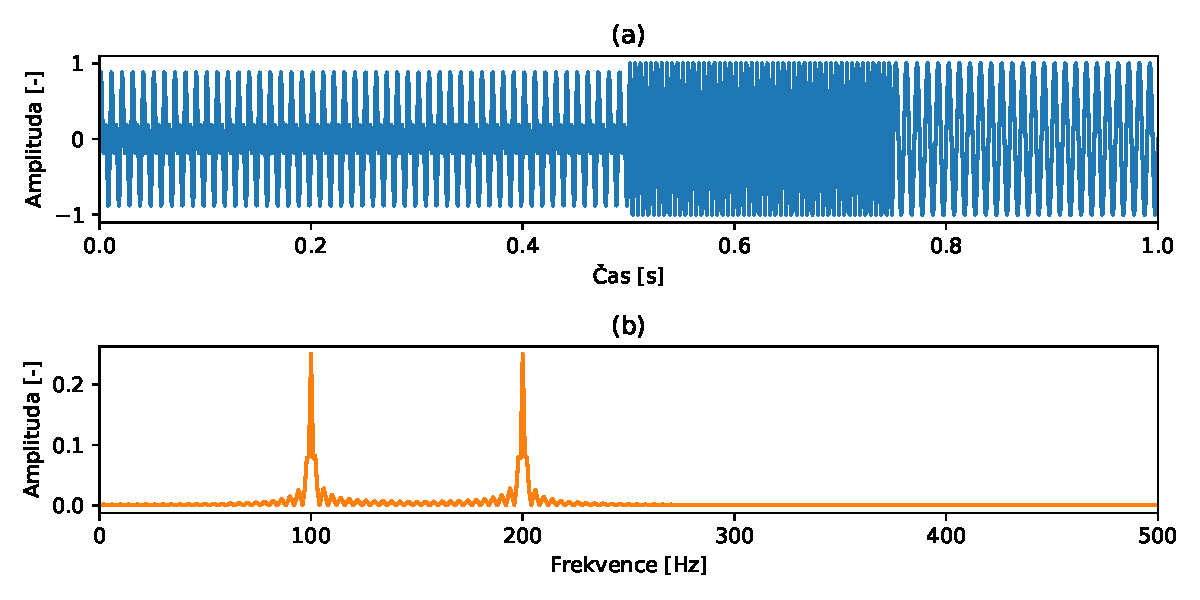
\includegraphics[width=\textwidth]{obrazky/casova_a_frekvencni_oblast.pdf}
    \caption{\textbf{Ukázka signálu v~časové a frekvenční oblasti.} (a) Zobrazení signálu složeného ze dvou sinusoid o~frekvenci 100 Hz a 200 Hz v~časové oblasti. (b) Zobrazení signálu z~obrázku (a) ve frekvenční oblasti. Z~obrázku je patrné, že signál obsahuje frekvence 100 Hz a 200 Hz, není však možné určit rozložení těchto frekvencí v~čase.}
    \label{obr_casova_a_frekvencni_oblast}
\end{figure*}

\begin{figure*}[h]
    \centering
    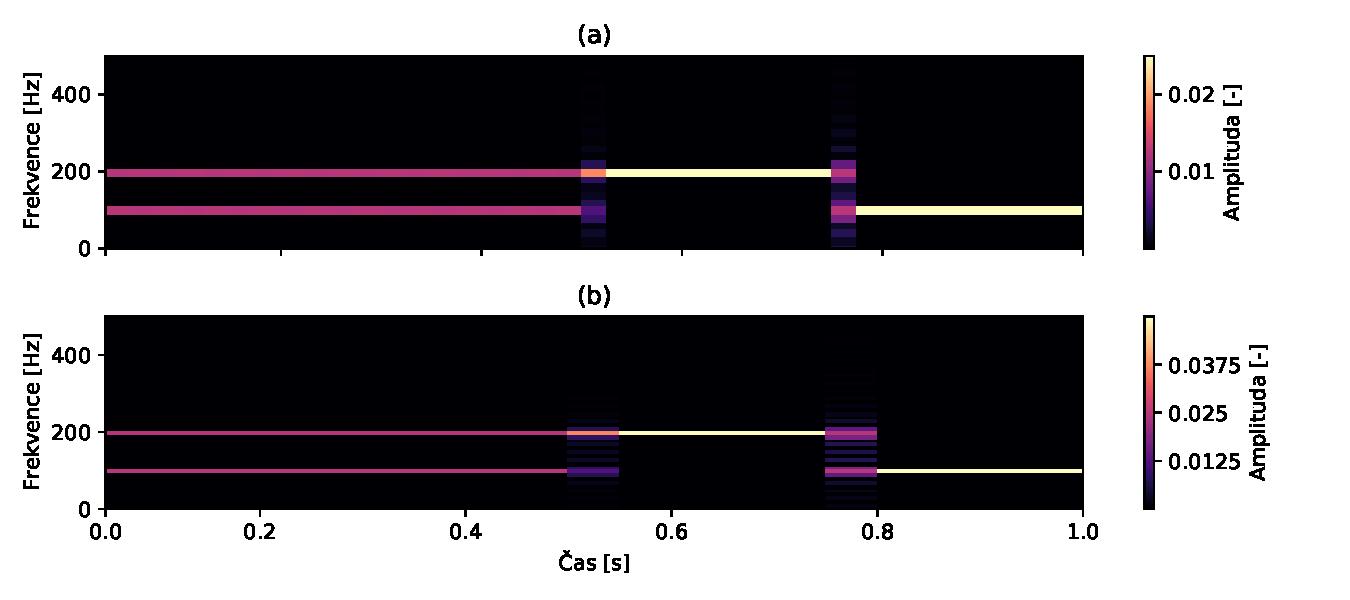
\includegraphics[width=\textwidth]{obrazky/spektrogramy.pdf}
    \caption{\textbf{Ukázka signálu v~časově-frekvenční oblasti.} Spektrogramy signálu z~obrázku~\ref{obr_casova_a_frekvencni_oblast}(a). Na rozdíl od zobrazení ve frekvenční oblasti je ze zobrazení v~časově-frekvenční oblasti možné rozpoznat rozložení frekvencí v~čase. Delší okno umožňuje přesněji určit frekvence, zatím co kratší okno umožňuje přesněji určit rozložení frekvencí v~čase. (a) Spektrogram se šířkou okna 1000 vzorků a posunem okna 500 vzorků. (b) Spektrogram se šířkou okna 2000 vzorků a posunem okna 1000 vzorků.}
    \label{obr_spektrogramy}
\end{figure*}

\clearpage

\subsection*{Nízkoúrovňové atributy}
\label{nizkourovnove_atributy}
Nízkoúrovňové atributy lze vypočítat přímo ze zvukové stopy, či odvozeně například z~její reprezentace ve frekvenční oblasti. Tyto atributy z~pohledu uživatelů nemají velký význam, avšak počítače je jsou schopny snadno využít a dále pomocí nich vypočítat atributy vyšší úrovně. Nízkoúrovňových atributů je mnoho, proto je dále přiblíženo jen několik z~nejpoužívanějších.\cite{MIR}

\subsubsection*{Mel-frekvenční kepstrální koeficienty}
\textit{Mel-frekvenční kepstrální koeficienty (Mel-frequency cepstrum coefficients, MFCC)} jsou kompaktní formou popisu spektra stopy. Jejich výpočet probíhá filtrováním frekvenčního spektra sadou trojúhelníkových filtrů s~šířkou pásma odpovídající \textit{Mel-frekvenční škále}. Tato škála byla vytvořena tak, aby simulovala vnímání frekvencí lidským uchem. Její nárůst je lineární po 1 kHz a dále logaritmický. Pro výpočet koeficientů je pro každý z~filtrů vypočítána pásmová energie odmocněním a sečtením amplitud odpovídající části spektra. Logaritmus této energie je nakonec zpracován pomocí \textit{Diskrétní kosinové transformace (Discrete cosine transform, DCT)}, čímž je snížena míra korelace pásem způsobená částečně se překrývajícími filtry. Výpočet \textit{MFCC} se u~hudebních souborů typicky provádí nad frekvenčními spektry každého z~oken spektrogramu, nikoli nad frekvenčním spektrem celé stopy. Schéma výpočtu Mel-frekvenčních kepstrálních koeficientů je možné vidět v~obrázku~\ref{obr_MFCC}.\cite{MIR}\cite{low_level}\cite{aca}

\begin{figure*}[h]
    \centering
    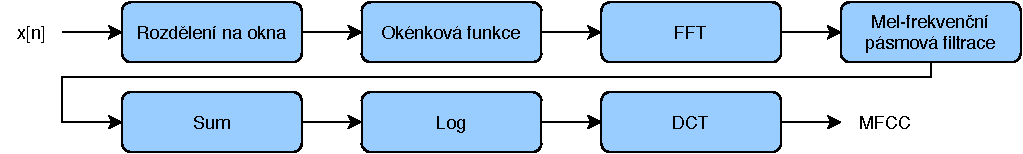
\includegraphics[width=\textwidth]{obrazky/MFCC.pdf}
    \caption{\textbf{Blokové schéma výpočtu Mel-frekvenčních kepstrálních koeficientů.} Obrázek znázorňuje výpočet \textit{MFCC} pro každé z~oken spektrogramu. \textit{FFT} značí rychlou Fourierovu transformaci, \textit{Sum} značí součet, \textit{Log} značí logaritmus a \textit{DCT} značí Diskrétní kosinovou transformaci.}
    \label{obr_MFCC}
\end{figure*}

\subsubsection*{Spektrální kontrast}
\textit{Spektrální kontrast (Spectral contrast)} vyjadřuje rozdíl energií mezi vrcholy a údolími spektra. Obdobně jako u~\textit{MFCC} je při výpočtu spektrálního kontrastu frekvenční spektrum zpracováno pomocí sady filtrů. U~spektrálního kontrastu však šířka pásma filtrů odpovídá oktávám chromatické stupnice. Pro každé z~pásem je pak vypočítán rozdíl energií mezi vrchním a spodním kvantilem spektra. Pokud jako $\{X_s[1], X_s[2], \dots , X_s[K]\}$ označíme sestupně seřazené hodnoty amplitud frekvencí filtračního pásma $s$ jednoho okna spektrogramu, pak rovnice pro výpočet spektrálního kontrastu $SC_s$ má tvar

\begin{equation}
	SC_s = log(\frac{1}{\alpha K} \sum\limits_{k=1}^{\alpha K} X_s[k]) - log(\frac{1}{\alpha K} \sum\limits_{k=1}^{\alpha K} X_s[K-k+1]),
\end{equation}

\medskip

\noindent kde $\alpha$ značí velikost kvantilů. Pro získání finálních hodnot spektrálního kontrastu jsou hodnoty $SC_s$ zpracovány pomocí \textit{Karhunen-Loeveovy transformace (Karhunen-Loeve transform, K-L)}. Schéma výpočtu Mel-frekvenčních kepstrálních koeficientů je možné vidět v~obrázku~\ref{obr_SC}.\cite{1035731}\cite{mircom}

\begin{figure*}[h]
    \centering
    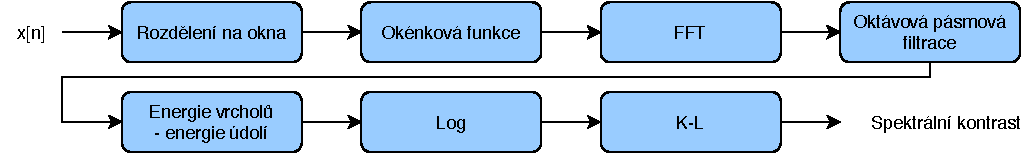
\includegraphics[width=\textwidth]{obrazky/SC.pdf}
    \caption{\textbf{Blokové schéma výpočtu spektrálního kontrastu.} Obrázek znázorňuje výpočet spektrálního kontrastu pro každé z~oken spektrogramu. \textit{FFT} značí rychlou Fourierovu transformaci, \textit{Log} značí logaritmus a \textit{K-L} značí Karhunen-Loeveovu transformaci.}
    \label{obr_SC}
\end{figure*}

\subsubsection*{Počet průchodů nulou}
\textit{Počet průchodů nulou (zero crossing rate (ZCR))} udává, kolikrát amplituda signálu změní znaménko z~pozitivního na negativní či naopak. U~úzkopásmových signálů jako jsou sinusoidy je hodnota \textit{ZCR} propojena s~jejich základní frekvencí. Tento atribut může být využit například při klasifikaci perkusních zvuků. Pokud jako $ZCR_r$ označíme počet průchodů nulou snímku $r$, rovnice pro výpočet pak má tvar

\begin{equation}
	ZCR_r = \frac{1}{2} \sum\limits_{n=1}^{N} | sign(x_r(n)) - sign(x_r(n-1)) |,
\end{equation}

\medskip

\noindent kde

\begin{equation}
    sign(x)=
    \begin{cases}
        1 \text{\qquad pro \quad} x \geq 0,\\
        -1 \text{\qquad pro \quad} x < 0. \text{\cite{MIR}\cite{zcr}\cite{low_level}\cite{mircom}\cite{aca}}
    \end{cases}
\end{equation}

\subsubsection*{Spektrální tok}
\textit{Spektrální tok (Spectral flux)} je atribut udávající míru korelace spekter po sobě jdoucích oken. Vysoké hodnoty spektrálního toku naznačují náhlou změnu amplitud spektra a tento atribut je tak možné využít k~detekci počátků událostí. Rovnice pro výpočet spektrálního toku $SF_r$ pro okno $r$ má tvar

\begin{equation}
	SF_r = \sum\limits_{k=1}^{K} {(|X_r(k))| - |X_{r-1}(k)|)}^2.\text{\cite{low_level}\cite{mgc}\cite{aca}}
\end{equation}

\subsubsection*{Spektrální centroid}
\textit{Spektrální centroid (Spectral centroid)} vyjadřuje geometrický střed distribuce spektra. Umístění centroidu ve vyšší části spektra značí přítomnost velkého počtu vysokých frekvencí. Rovnice pro výpočet centroidu má tvar

\begin{equation}
	SC_r = \frac{\sum\limits_{k=1}^{K} X_r[k] \cdot k}{\sum\limits_{k=1}^{K} X_r[k]}.\text{\cite{low_level}\cite{mgc}\cite{mircom}\cite{aca}}
\end{equation}

\subsubsection*{Spektrální klesání}
\textit{Spektrální klesání (Spectral roll-off)} udává frekvenci, pod kterou spadá většina energie spektra. Většinou se uvádí hodnota 85 \%. Z~matematického hlediska se jedná o~nejvyšší frekvenci $R_r$, pro kterou platí

\begin{equation}
	\sum\limits_{k=1}^{R_r} X_r[k] \leq 0.85 \cdot \sum\limits_{k=1}^{K} X_r[k].\text{\cite{low_level}\cite{mgc}\cite{mircom}\cite{aca}}
\end{equation}

\subsection*{Vysokoúrovňové atributy}
\label{vysokourovnove_atributy}
Vysokoúrovňové atributy popisují vlastnosti stopy snadno interpretovatelné lidmi. Jde například o~důležité vlastnosti stopy z~pohledu hudební teorie, jako jsou melodie, harmonie či rytmus. Může se ale jednat i o~více abstraktní atributy jako je například hodnota udávající vhodnost skladby k~tanci. Pro extrakci melodie a harmonie je nejprve nutné vybrat vhodnou metodu pro extrakci výšky tónů. Dále také některou z~metod pro detekci počátků událostí, která se používá i pro extrakci atributů týkajících se rytmu.\cite{MIR}\cite{aca}

\subsubsection*{Melodie a harmonie a rytmus}
\label{melodie_a_harmonie_a_rytmus}
Pro extrakci výšky tónů u~monofonních signálů se nejčastěji používají metody pro měření periodicity signálu, a to pomocí měření korelace vybraných atributů v~navazujících časových úsecích. Je také možné se setkat s~aproximací výšky pomocí ideální harmonické řady. U~polyfonních signálů se pro aproximaci všech výšek tónů nejčastěji používají iterativní metody aproximace výšky dominantního tónu nalezením nejvýraznější základní frekvence a její harmonické řady. Tyto jsou následně odečteny od původního spektra stopy a proces je opakován, dokud nejsou aproximovány výšky všech tónů. Další způsoby spočívají v~nalezení takové sady základních frekvencí a jejich harmonických řad, pomocí které je co nejpřesněji možné aproximovat původní spektrum.\cite{MIR}\cite{low_level}\cite{aca}

Pro následnou extrakci atributů týkajících se melodie či rytmu se používají algoritmy pro detekci počátků událostí. Tyto počátky se většinou vyznačují náhlým nárůstem amplitudy a jejich detekce tak probíhá sledováním výrazných změn energie v~časové oblasti, případně také nárůstu vysokofrekvenčních komponent. U~současných systémů pro detekci počátků je největší limitací obtížná detekce počátků u~zvukových stop, které neobsahují zdroj výrazných změn amplitud, jako jsou například perkusní nástroje. V~takovém případě pro detekci počátků mohou být využity právě hodnoty výšek tónů, kde jejich změna může značit počátek události.\cite{MIR}\cite{aca}

Výše zmíněné postupy je pak možné využít k~extrakci atributů vyšší úrovně týkajících se melodie či rytmu. U~extrakce melodie je stopa rozdělena na segmenty na základě detekovaných počátků. Pro každý segment je pak provedena detekce výšek tónů. Výsledkem je řada různých po sobě jdoucích tónu značící melodii. Detekce počátků se používá i pro extrakci atributů týkajících se rytmu. Tempo skladby je aproximováno pomocí měření periodicity těchto počátků, často je však výsledkem násobek tempa reálného, například kvůli detekci půldob. Počátky mohou být využity i pro detekci úderů perkusních nástrojů. Obrázek~\ref{obr_detekce_pocatku_a_not} znázorňuje detekci počátků a not.\cite{MIR}\cite{aca}

\begin{figure*}[h]
    \centering
    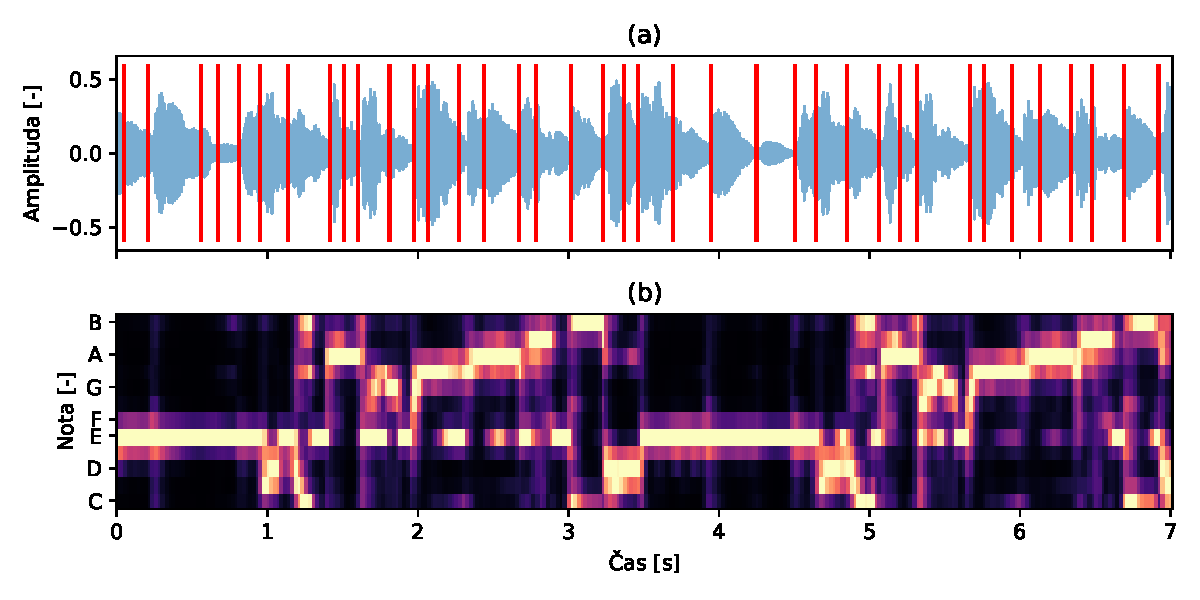
\includegraphics[width=\textwidth]{obrazky/detekce_pocatku_chroma.pdf}
    \caption{\textbf{Ukázka detekce počátků událostí a not.} (a) Detekované počátky událostí, vyznačující se náhlou změnou amplitudy, jsou znázorněny svislými červenými čarami. (b) Vyšší intenzita detekovaných not je znázorněna světlejší barvou. Po sobě jdoucí noty pak značí detekovanou melodii.}
    \label{obr_detekce_pocatku_a_not}
\end{figure*}

\section{Selekce atributů}
\label{selekce_atributu}
Selekce atributů je dalším ze způsobů dimenzionální redukce a steně jako u~extrakce atributů je jejím cílem odstranit redundantní či irelevantní data. Na rozdíl od extrakce atributů, jejíž výstupem jsou transformovaná data pomocí funkcí, výstupem této metody je podmnožina dat původních. Selekci je možné provádět manuálně či algoritmicky, dále bude rozebrána pouze druhá z~těchto variant. Metody selekce je možné rozdělit na základě jejich přístupu k~vyhodnocení vhodných atributů, a to na metody filtrační, obalovací a vestavěné. Diagram těchto metod je možné vidět v~obrázku~\ref{obr_selekce_atributu}.\cite{data_classification}\cite{aca}

\subsection*{Filtrační metody}
\label{filtracni_metody}
Filtrační metody se skládají ze dvou kroků, kde v~prvním kroku je vhodnost atributů vyhodnocena pomocí některé z~metrik jako \textit{vzdálenost}, \textit{korelace}, \textit{vzájemná informace} nebo \textit{konzistence}. V~druhém kroku je pak vybrán stanovený počet atributů s~nejvyšším hodnocením pro předání klasifikačním algoritmům. Atributy mohou být vyhodnoceny samostatně nebo v~kontextu množiny atributů, kde v~druhém případě jsou pak metody schopny rozpoznat redundantní data. Tyto metody nezávisí na žádném klasifikačním algoritmu a jsou tak obecně schopny lépe popsat vztah mezi atributy.\cite{data_classification}\cite{data_preprocessing}\cite{aca}

\subsection*{Obalovací metody}
\label{obalovaci_metody}
Obalovací metody využívají k~ohodnocení atributů chybovost predikce určitého modelu. Berou tedy v~potaz, že každý klasifikátor může dosáhnout nejlepších výsledků pomocí odlišných atributů. V~prvním kroku metody vybírají podmnožiny z~množiny atributů za pomoci nějakého z~vyhledávacích algoritmů a v~druhém kroku je předají modelu k~ohodnocení pomocí chybovosti predikce. Tento proces je opakován, dokud není nalezena podmnožina dosahující nejvyšší úspěšnosti, či úspěšnosti převyšující stanovenou hranici. Vzhledem k~nutnosti natrénovat model pro každou z~podmnožin atributů jsou tyto metody velmi výpočetně náročné. Lze však pomocí nich pro daný model dosáhnout vyšší úspěšnosti klasifikace, než pomocí metod filtračních.\cite{data_classification}\cite{data_preprocessing}\cite{aca}

\subsection*{Vestavěné metody}
\label{vestavene_metody}
Vestavěné metody stejně jako metody obalovací pro vyhodnocení vhodnosti atributů využívají vybraného prediktivního modelu, na rozdíl od metod obalovacích jsou však přímo jeho součástí. Selekce probíhá již při konstrukci modelu a není tak nutné jej opakovaně trénovat. Vestavěné metody lze rozdělit na tři varianty podle postupu selekce, který využívají. První varianta těchto metod natrénuje model na všech atributech a následně nastavením koeficientů či vah náležícím k~vybraným atributům testuje, zda-li jejich absence má vliv na úspěšnost predikce modelu. Další variantou je využití algoritmů jako \textit{ID3} či \textit{C4.5} pro výběr atributů, jako je tomu u~rozhodovacích stromů. Poslední variantou je pak regularizace pomocí penalizačních funkcí, které na základě vybraného kritéria již v~průběhu trénování snižují koeficienty či váhy vybraných atributů.\cite{data_classification}

\begin{figure}[h]
    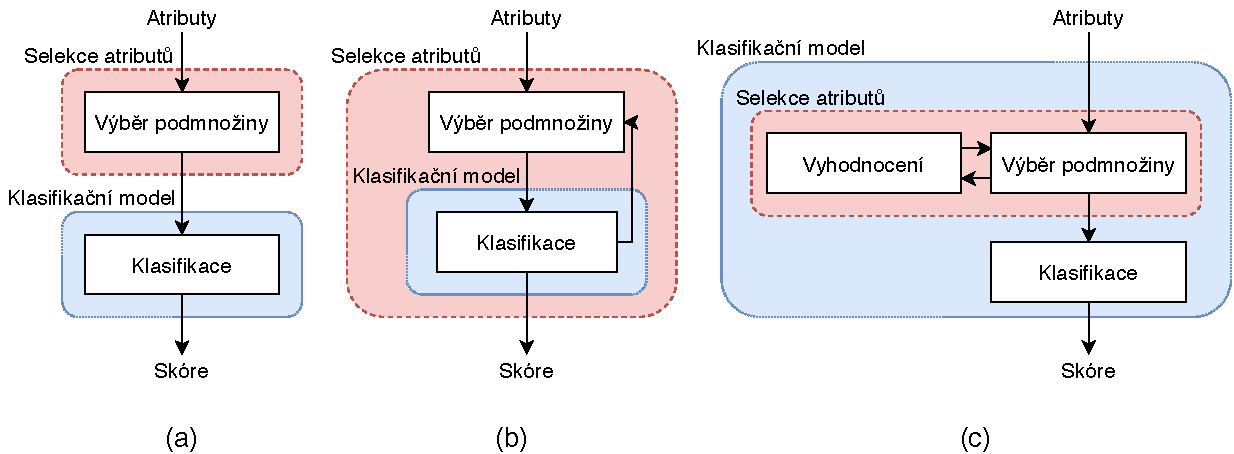
\includegraphics[width=\textwidth]{obrazky/selekce_atributu.pdf}
    \caption{\textbf{Diagram metod selekce atributů.} (a) Diagram průběhu filtračních metod. Selekce probíhá zcela nezávisle na vybraném klasifikačním algoritmu. (b) Diagram obalovacích metod. Úspěšnost selekce je vyhodnocována pomocí vybraného klasifikačního algoritmu. Není však jeho součástí. (c) Diagram vestavěných metod. Selekce je přímo součástí klasifikačního algoritmu.}
    \label{obr_selekce_atributu}
\end{figure}

\section{Kódování kategorických dat}
\label{kodovani_kategorickych_dat}
Kategorická data často bývají ve formě textových řetězců, a protože většina klasifikátorů textová data zpracovat neumí, může být nutné je nejprve převést do číselné podoby. Nejprve je potřeba určit, jestli kategorická data jsou ordinální či nominální. Nominální kategorická data jsou taková, která mezi sebou nelze porovnat, protože nezastávají žádnou hodnotu. Příkladem nominálních kategorických dat může být například barva. Oproti tomu ordinální data lze porovnat nebo je seřadit. Příkladem ordinálních dat může být například vzdělání, kde vysokoškolské vzdělání má vyšší hodnotu, než vzdělání středoškolské. Nominální kategorická data není vhodné zakódovat tak, aby výsledné hodnoty byly ordinální. V~následujících odstavcích jsou popsány nejpoužívanější způsoby kódování. Ukázky kódování kategorických dat je možné vidět v~tabulce~\ref{ukazka_kodovani_kategorickyc_dat}.\cite{cat_var_enc1}

\textit{Ordinální kódování (ordinal encoding)} je vhodné pro ordinální data a funguje na principu přiřazení unikátní číselné hodnoty každé z~možných kategorických hodnot. Tato přiřazená číselná hodnota musí odpovídat důležitosti původní kategorické hodnoty. Výhodou tohoto způsobu kódování je, že nezvyšuje velikost dat.\cite{cat_var_enc1}

\textit{Binární kódování (Binary encoding)} nejprve transformuje atributy na jejich číselné reprezentace, následně tyto převede do binární podoby a nakonec vytvoří vektor jedniček a nul pro každý řád hodnot binární reprezentace. Výsledkem je tedy vektor o~délce počtu prvků v~kódovaných datech a počet těchto vektorů je $log_2(N)$, kde $N$ vyjadřuje počet unikátních kategorických hodnot.\cite{cat_var_enc2}

\textit{One-hot kódování (One-hot encoding)} transformuje každou kategorickou hodnotu na vektor jedniček a nul od délce rovné počtu prvků v~kódovaných datech, kde jednička u~příslušného prvku značí přítomnost dané kategorické hodnoty a nula naopak. Pokud označíme počet unikátních kategorických hodnot písmenem $N$, výsledný počet těchto vektorů bude $N-1$, protože jeden z~vektorů je vždy možné odvodit z~vektorů ostatních a typicky tak bývá odstraněn. Nevýhody tohoto kódování spočívají ve velkém nárůstu dat a s~tím spojenou možností představení fenoménu \textit{řídkých dat (sparse data)}. Tento způsob kódování tak není vhodné použít pro velký počet kategorických dat.\cite{cat_var_enc1}\cite{cat_var_enc2}

\begin{table}[H]
	\vskip6pt
	\caption{\textbf{Ukázka kódování kategorických dat}}
    \vskip6pt
	\centering
    \begin{tabularx}{\textwidth}{ |l|l| *{5}{Y|} }
        \hline
        Původní hodnota & Ordinální kódování & \multicolumn{2}{l|}{Binární kódování} &  \multicolumn{3}{l|}{One-hot kódování} \\ \hline
        \hline
        a & 0 & 0 & 0 & 0 & 0 & 0 \\ \hline
        b & 1 & 0 & 1 & 1 & 0 & 0 \\ \hline
        c & 2 & 1 & 0 & 0 & 1 & 0 \\ \hline
        d & 3 & 1 & 1 & 0 & 0 & 1 \\ \hline
    \end{tabularx}
    \label{ukazka_kodovani_kategorickyc_dat}
\end{table}

\section{Škálování dat}
\label{skalovani_dat}
Vstupní data často bývají ve formě, kde hodnoty jednoho atributu jsou řádově jinde, než hodnoty atributu jiného. Některé z~klasifikačních algoritmů pak mohou mít problém takovým atributům přiřadit adekvátní váhu. Z~tohoto důvodu se v~praxi můžeme u~předzpracování dat setkat se \textit{škálováním dat (data scaling)}. V~následujících odstavcích jsou dále přiblíženy nejpoužívanější z~těchto metod. Metody škálování dat jsou znázorněny v~obrázku~\ref{obr_sklaovani_dat}.\cite{data_mining}\cite{data_preprocessing}

Jedna z~metod škálování je metoda \textit{min-max normalizace}, kde jsou data lineárně transformována do určitého intervalu, obvykle $\langle$0, 1$\rangle$. Rovnice pro převod hodnoty $x_i$ z~množiny $X$ do intervalu $\langle$a, b$\rangle$ má tvar

\begin{equation}
	x'_i = a + \frac{(x_i - min(X)) (b-a)}{max(X) - min(X)},
\end{equation}

\medskip

\noindent kde funkce $min()$ a $max()$ vracejí nejnižší a nejvyšší hodnotu ze vstupní množiny. Tato metoda je však citlivá na \textit{odlehlé hodnoty (outliers)}.\cite{data_mining}\cite{data_preprocessing}

Další metoda se nazývá \textit{Z-score normalizace} jejím cílem je transformovat vstupní hodnoty tak, aby jejich průměr byl roven nule a směrodatná odchylka rovna jedné. Rovnice Z-score normalizace má tvar

\begin{equation}
	x'_i = \frac{x_i - mean(X)}{std(X)},
\end{equation}

\medskip

\noindent kde funkce $mean()$ vrací průměrnou hodnotu a funkce $std()$ vrací hodnotu směrodatné odchylky vstupního vektoru hodnot.\cite{data_mining}\cite{data_preprocessing}

\begin{figure}[h]
    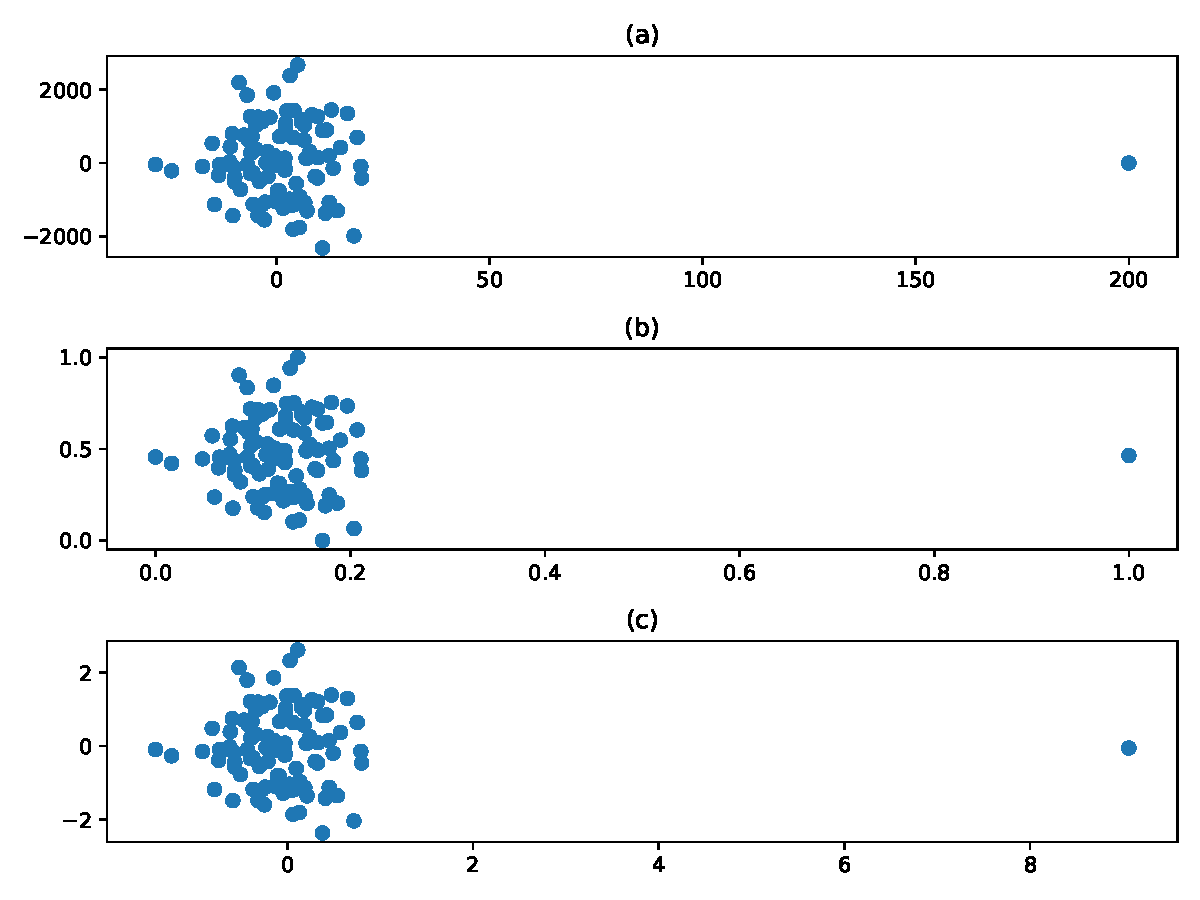
\includegraphics[width=\textwidth]{obrazky/skalovani.pdf}
    \caption{\textbf{Ukázka metod škálování dat.} (a) Znázornění neupravených hodnot atributů v~prostoru prvků. Většina hodnot na ose $y$ spadá do rozmezí ($-2000$--$2000$) a většina hodnot na ose $x$ spadá do rozmezí ($-25$--$25$). Zatím co nárůst hodnoty o~$10$ bude na ose $x$ podstatný, stejný nárůst bude na ose $y$ poměrně zanedbatelný. (b) Data transformovaná metodou \textit{min-max normalizace}. Zatím co většina hodnot na ose $y$ spadá do rozmezí ($0.2$--$0.8$), odlehlá hodnota na ose $x$ způsobila, že většina hodnot na ose $x$ spadá do rozmezí ($0$--$0.2$). Nárůst o~stejnou hodnotu bude tedy stále podstatně výraznější na ose $x$. (c) Data transformovaná metodou \textit{Z-score normalizace}. Většina hodnot na obou dvou osách spadá do rozmezí ($-2$--$2$), nárůst o~stejnou hodnotu je tedy na obou osách srovnatelný.}
    \label{obr_sklaovani_dat}
\end{figure}

\chapter{Klasifikační algoritmy}
\label{klasifikacni_algoritmy}
Klasifikace je proces učení s~učitelem, tedy algoritmy při učení pracují s~daty rozdělenými do tříd, u~kterých jsou známé jejich správné hodnoty. Cílem tohoto učení je vytvořit funkci, která bude na základě určitých vlastností dat shopna správně určit třídu, do které tato data patří. Výsledná funkce se pak nazývá klasifikační model (klasifikátor). Cílem klasifikace je vytvořit takový model, který bude schopný rozřadit neznámá data do tříd s~co nejvyšší úspěšností. To však vyžaduje, aby byl model schopný generalizovat, tedy brát v~potaz to, že u~neznámých dat mohou pro klasifikaci být důležité jiné z~vlastností, než u~dat známých, na kterých byl natrénován. V~případě, kdy je model schopný klasifikovat trénovací data s~velmi vysokou úspěšností, avšak u~dat neznámých dosahuje podstatně nižší úspěšnosti, se nazývá \textit{přetrénování (overfitting)}. V~následujících podkapitolách je přiblíženo několik z~nejznámějších klasifikátorů. Speciálním případem je pak takzvaný meta-klasifikátor, což je klasifikátor využívající několik klasifikátorů dohromady. Metody využívající meta-klasifikátory se nazývají \textit{ensemble metody} a jsou rozebrány v~poslední podkapitole.\cite{data_classification}

\section{Pravděpodobnostní metody}
\label{pravdepodobnostni_metody}
\textit{Pravděpodobnostní metody (Probabilistic methods)} využívají principů statistiky pro klasifikaci dat. Cílem těchto metod je pro každou vstupní položku $X$ nalézt takovou třídu $C_k$ z~$K$ tříd, pro kterou je pravděpodobnost, že k~ní náleží, nejvyšší. V~následujících odstavcích jsou krátce popsány dva nejznámější klasifikátory využívající pravděpodobnostních metod pro klasifikaci položek.\cite{data_classification}

\textit{Naivní Bayesův klasifikátor (Naive Bayes classifier)} je generalizační model, který pro klasifikaci využívá Bayesova teorému. Naivní se nazývá pro to, že předpokládá takzvanou \textit{podmíněnou nezávislost}. Tedy, pokud je již dána třída, předpokládá, že všechny atributy klasifikovaného prvku jsou vzájemně nezávislé. Pokud jako $x_n$ označíme $n$-tý z~$N$ atributů klasifikovaného prvku $X$, pak rovnice Naivního Bayesova klasifikátoru má tvar

\begin{equation}
	NB(X) = \underset{C_k}{argmax}(P(C_k) \prod\limits_{n=0}^{N-1} P(x_n|C_k)).\text{\cite{data_classification}\cite{machine_learning}}
\end{equation}

\medskip

\textit{Logistická regrese (Logistic regression)} je metoda binární klasifikace, jejíž cílem je nalézt vhodnou diskriminační funkci, pomocí které je na základě vektoru atributů klasifikovaného prvku možné určit, zda náleží k~vybrané třídě, či nikoliv. Rovnice logistické regrese má tvar

\begin{equation}
    P(Y=1|X) = g(\theta^T X) = \frac{1}{1-e^{-\theta^T X}},
\end{equation}

\medskip

\noindent kde 

\begin{equation}
    g(z) = \frac{1}{1-e^{-z}}
\end{equation}

\medskip

\noindent se nazývá logistická funkce a platí

\begin{equation}
    \theta^T X = \theta_0 + \sum\limits_{n=0}^{N-1} \theta_{n+1} x_n,
\end{equation}

\medskip

\noindent kde $\{\theta_0, \dots, \theta_N\}$ značí parametry logistické funkce. Pro nalezení adekvátních hodnot těchto parametrů se používá \textit{metoda maximální věrohodnosti}. Pro klasifikaci do více tříd lze využít metodu \textit{jeden proti všem (one-vs-all)}, nebo upravenou verzi logistické regrese nazývanou \textit{Multinomiální logistická regrese}.\cite{data_classification}\cite{understanding_machine_learning}

\section{Rozhodovací stromy}
\label{rozhodovaci_stromy}
\textit{Rozhodovací stromy (Decision trees)} rekurzivním dělením transformují vstupní data do stromové struktury, kde každý z~koncových uzlů je přiřazen k~určité třídě. Existuje několik algoritmů pro automatickou generaci rozhodovacích stromů, jako například algoritmy \textit{ID3}, \textit{C4.5} a \textit{CART}. Dělení každého z~vnitřních uzlů probíhá na základě \textit{dělícího kritéria (split criterion)}, které pomocí podmínky či predikátu vyhodnotí buďto hodnotu jednoho z~atributů, pak se jedná o~univariační dělení, nebo hodnoty více atributů, pak se jedná o~multivariační dělení. Cílem tohoto dělení je maximalizovat příslušnost prvků v~každém poduzlu k~určité třídě. Vhodnost atributů k~dělení se vyhodnocuje pomocí různých funkcí jako jsou \textit{entropie} či \textit{Gini index}. Entropie a Gini index se počítají podle vzorců

\begin{equation}
    Entropie = - \sum\limits_{k=0}^{K-1} p(C_k) log_2 p(C_k)
\end{equation}

\medskip

\noindent a

\begin{equation}
    Gini = 1 - \sum\limits_{k=0}^{K-1} p(C_k)^2,
\end{equation}

\medskip

\noindent kde $p(C_k)$ vyjadřuje pravděpodobnost klasifikace do třídy $C_k$ z~celkového počtu $K$ tříd. Entropie se používá pro výpočet informačního zisku, který pro vyhodnocení vhodnosti atributu pro dělení uzlu používají algoritmy \textit{ID3} a \textit{C4.5}. Gini index pak pro toto vyhodnocení používá algoritmus \textit{CART}.

Dělení uzlů probíhá, dokud není splněno jedno z~ukončovacích kritérií. Ukončovacím kritériem může být například náležitost všech prvků v~uzlu ke stejné třídě. V~praxi se však obvykle používají jiná kritéria, jako náležitost určité části prvků uzlu ke stejné třídě, či pouze určitý počet prvků v~uzlu. Tyto navíc pomáhají zamezit přetrénovaní modelu. Není však možné předem určit hodnoty těchto kritérií tak, aby byl růst stromu zastaven ve vhodnou chvíli. Tento problém řeší metoda \textit{prořezávání stromu (tree pruning)}, která zpětně prochází vytvořený strom a odstraňuje uzly, které by k~přetrénování mohly vést. Jedním ze způsobů prostřihávání stromů je vyčlenění části trénovacích dat a jejich následné použití při vyhodnocování úspěšnosti klasifikace stromů po odstranění určitých uzlů.\cite{data_classification}\cite{understanding_machine_learning}\cite{strojove_uceni}\cite{machine_learning}

\section{Učení založené na instancích}
\label{uceni_zalozene_na_instancich}
Metody \textit{učení založené na instancích (instance based learning)} fungují na principu vyhodnocení podobnosti klasifikovaného prvku mezi již známými prvky (instancemi) z~trénovacích dat, a to za pomoci vybrané metriky. Tyto metody na základě trénovacích dat nevytváří model, pouze tato data uloží a samotná klasifikace proběhne až ve chvíli, kdy je metodě předán prvek z~dat testovacích. Tento přístup se nazývá \textit{líné učení (lazy learning)}. Tyto metody mají řadu výhod, jednak pro klasifikaci využívají pouze část všech dat, což umožňuje snadněji klasifikovat velmi rozsáhlá data, dále každý nový prvek z~testovacích dat je možné zařadit mezi již známé prvky dat trénovacích. To může vylepšit úspěšnost klasifikace a také umožní klasifikovat i třídy, které trénovací data neobsahovala. Mezi nevýhody tohoto přístupu se řadí vysoká citlivost na irelevantní data a nevyváženost počtu prvků v~jednotlivých třídách.\cite{data_classification}\cite{machine_learning}\cite{strojove_uceni}

Nejznámější z~metod založených na instancích je metoda \textit{K-nejbližších sousedů (K-nearest neighbors)}. Tato metoda je založena na předpokladu, že podobnost dvou prvků může být vyjádřena pomocí jejich vzdálenosti v~prostoru prvků. Metrikou pro vyhodnocení podobnosti je například \textit{Euklidovská vzdálenost}, jejíž rovnice má tvar

\begin{equation}
    d(X, Y) = \sqrt{\sum\limits_{n=0}^{N-1} ((x_n)-(y_n))^2},
\end{equation}

\medskip

\noindent kde $d(X, Y)$ značí výslednou vzdálenost mezi prvkem $X$ s~atributy $\{x_0, \dots, x_{N-1}\}$ a prvkem $Y$ s~atributy $\{y_0, \dots, y_{N-1}\}$. Při klasifikaci nového prvku tato metoda pomocí dané metriky nalezne $k$ nejbližších prvků, a na základě nejčastěji se vyskytující třídy mezi těmito prvky přiřadí třídu prvku novému. Princip fungování metody K-nejbližších sousedů je znázorněn v~obrázku~\ref{obr_knn}.\cite{strojove_uceni}\cite{machine_learning}

\begin{figure*}[h]
    \centering
    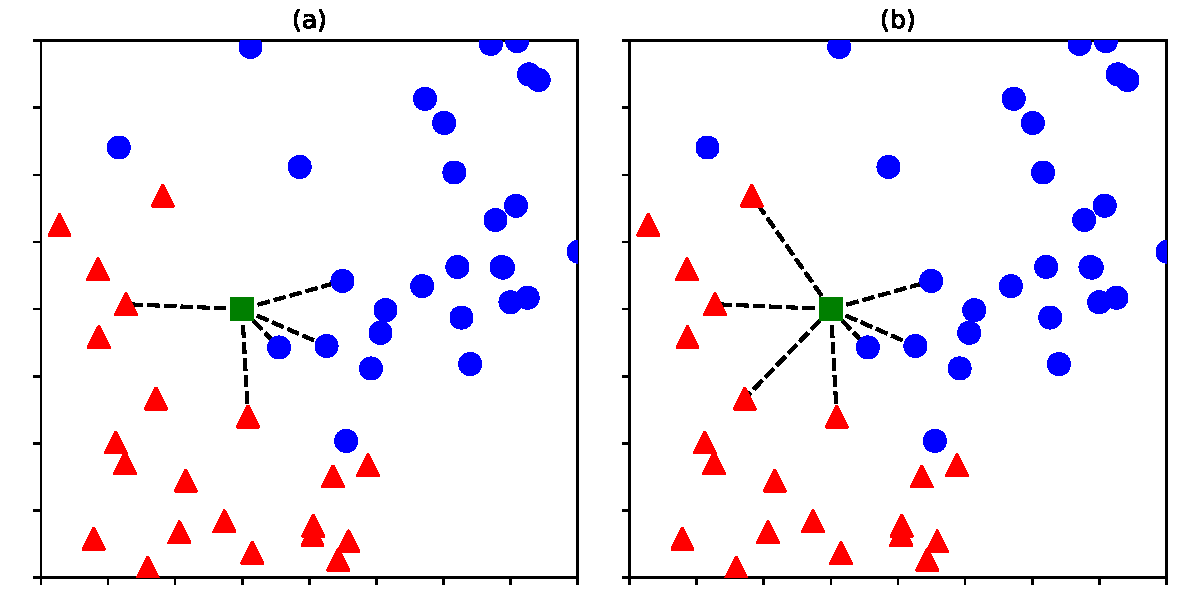
\includegraphics[width=\textwidth]{obrazky/knn.pdf}
    \caption{\textbf{Ukázka klasifikace pomocí metody K-nejbližších sousedů.} V~obrázcích je znázorněn prostor prvků definovaný dvěma atributy. (a) Ukázka metody s~hodnotou $k = 5$. Klasifikovaný prvek reprezentovaný zeleným čtvercem by v~tomto případě byl klasifikován jako modrý kruh. (b) Ukázka metody s~hodnotou $k = 7$. Klasifikovaný prvek reprezentovaný zeleným čtvercem by v~tomto případě byl klasifikován jako červený trojúhelník.}
    \label{obr_knn}
\end{figure*}

\section{Metody podpůrných vektorů}
\label{metody_podpurnych_vektoru}
\textit{Metody podpůrných vektorů (Support vector machines, SVM)} separují dvě třídy pomocí stanovení lineární rozhodovací hranice (nadroviny) tak, aby na každé její straně ležely prvky náležící ke stejné třídě. Jedná se tedy o~binární klasifikaci a pro klasifikaci do více tříd je možné využít metodu jeden proti všem. V~případě, kdy jsou prvky lineárně separovatelné, se pro stanovení hranice používá metoda nazývaná \textit{hard-margin}. Pomocí této metody je nadrovina umístěna tak, aby byl maximalizován její odstup od prvků každé z~tříd. Taková nadrovina se pak nazývá \textit{nadrovina maximálního odstupu (maximum margin hyperplane)} a prvky, na základě kterých byla pozice nadroviny stanovena, se nazývají \textit{podpůrné vektory (support vectors)}.\cite{data_classification}\cite{understanding_machine_learning}

V~případě, kdy prvky nejsou lineárně separovatelné, ale přesto je možné umístit lineární rozhodovací hranici tak, aby pomocí ní bylo možné prvky klasifikovat s~uspokojivou úspěšností, je možné použít metodu nazývanou \textit{soft-margin}. Vhodnost umístění nadroviny touto metodu je vyhodnocena pomocí funkcí, které kladně hodnotí správně klasifikované prvky splňující stanovený odstup od hranice, ale záporně hodnotí prvky, které odstup nesplňují, či hranici překročí a jsou tak chybně klasifikovány.

V~případě, kdy jsou prvky lineárně neseparovatelné a není možné umístit nadrovinu tak, aby bylo dosaženo dostatečné úspěšnosti klasifikace, je možné využít některé z~\textit{jádrových metod (kernel methods)}. Tyto metody transformují prostor prvků na jiný, obvykle vícedimenzionální prostor, který umožňuje umístit nadrovinu tak, aby úspěšnost klasifikace byla uspokojivá. Protože však transformace prvků do nového prostoru není lineární, rozhodovací hranice v~původním prostoru bude také nelineární, jak je možné vidět v~obrázku~\ref{obr_svm}.

\begin{figure*}[h]
    \centering
    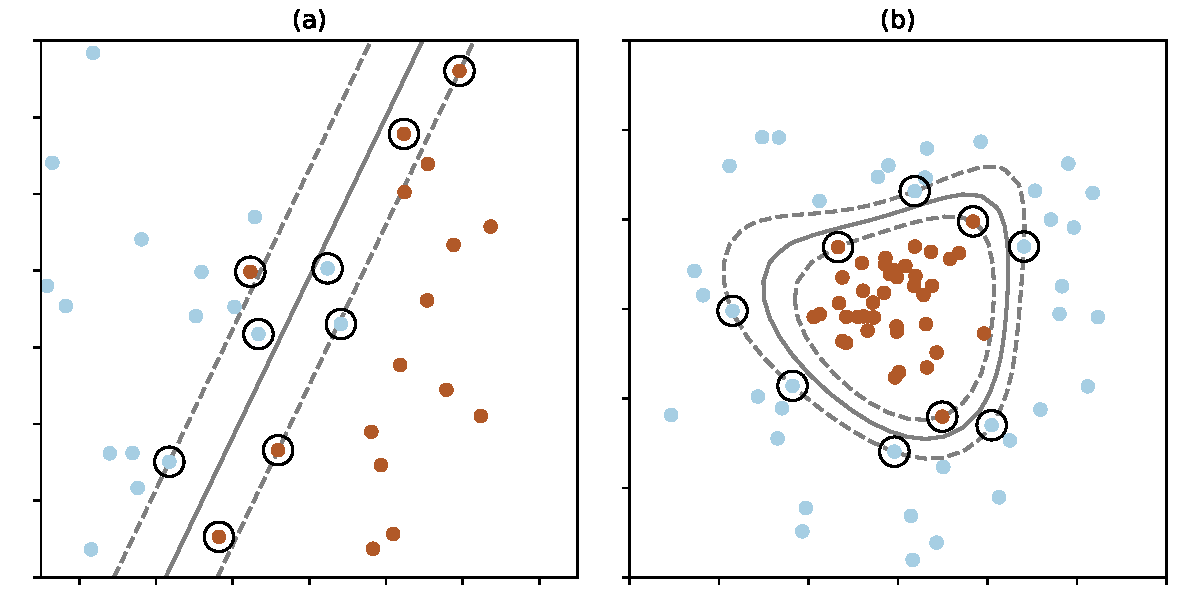
\includegraphics[width=\textwidth]{obrazky/svm.pdf}
    \caption{\textbf{Ukázka umístění nadroviny metodou podpůrných vektorů.} (a) Přesto, že data nejsou lineárně separovatelná je možné pomocí metody \textit{soft-margin} umístit nadrovinu tak, aby rozdělila prvky obou tříd s~uspokojivou úspěšností. (b) Ukázka případu, kdy ani pomocí metody \textit{soft-margin} není možné umístit nadrovinu tak, aby bylo dosaženo uspokojivé úspěšnosti klasifikace. Umístění nadroviny po transformaci prostoru prvků pomocí jádrové metody \textit{Radial basis function (RBF)} je však možné všechny prvky klasifikovat správně. Protože však tato transformace není lineární, po zpětné transformaci na původní prostor prvků je i stanovená hranice nelineární.}
    \label{obr_svm}
\end{figure*}

\section{Neuronové sítě}
\label{neuronove_site}
\textit{Neuronové sítě (Neural networks)} simulují biologické struktury lidského mozku. Architekturu neuronových sítí tvoří neurony a propojení mezi nimi. Neurony se podle funkce, kterou v~síti vykonávají, dělí na vstupní, výstupní a výpočetní. Mohou však plnit více funkcí najednou. Výpočetní neurony jsou základní výpočetní jednotky neuronových sítí. Jejich vstupem je několik hodnot a jim přiřazených vah, které transformují na výstupní hodnotu pomocí dvou funkcí. První funkce zpracuje vstupní hodnoty a váhy výsledek předá druhé funkci, která se nazývá \textit{aktivační funkce (activation function)}, která jej transformuje na výstupní hodnotu neuronu. Model neuronu je možné vidět v~obrázku~\ref{obr_neuron}.\cite{data_classification}\cite{machine_learning}

Neuronová síť se obvykle skládá z~několika vrstev, a to vrstvy vstupní, vrstev skrytých a vrstvy výstupní. Trénování takovýchto neuronových sítí pak probíhá ve dvou fázích, kde v~první se vstupní hodnoty postupně transformují a propagují dále v~síti až do výstupní vrstvy a v~druhé se v~případě chybné klasifikace upraví váhy příslušných neuronů pomocí metody zpětné propagace. Rychlost trénování je možné ovlivnit pomocí parametru $\lambda$. V~praxi se nejdříve parametru $\lambda$ přiřadí vyšší hodnota, což vede k~rychlejšímu nalezení hodnot vah blízkých hodnotám optimálním a následně se $\lambda$ snižuje, kvůli zabránění oscilace okolo těchto optimálních hodnot.\cite{data_classification}\cite{machine_learning}

Pro klasifikaci do více tříd pak lze využít metodu jeden proti všem, nebo navrhnout architekturu sítě tak, aby počet neuronů ve výstupní vrstvě odpovídal počtu klasifikovaných tříd. Výhody neuronových sítí spočívají jejich široké oblasti uplatnění, schopnosti zpracovat rozsáhlá data a jejich schopnosti implicitně provádět dimenzionální redukci. Nevýhody spočívají ve vyšší citlivosti na irelevantní data a možnosti přetrénování.\cite{data_classification}\cite{machine_learning}

\begin{figure*}[h]
    \centering
    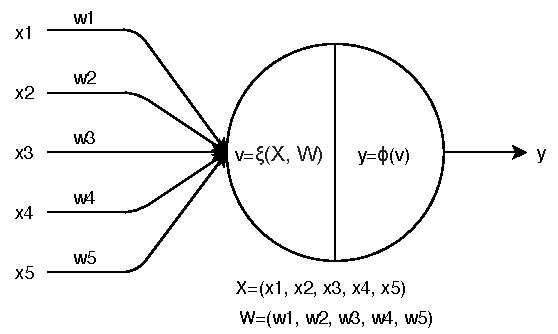
\includegraphics[width=0.49\textwidth]{obrazky/neuron.pdf}
    \caption{\textbf{Model neuronu.} Množina $X$ značí vstupní hodnoty neuronu, množina $W$ značí váhy pro každou ze vstupních hodnot.}
    \label{obr_neuron}
\end{figure*}

\section{Ensemble metody}
\label{ensemble_metody}
Ensemble metody využívají různé způsoby kombinování několika klasifikátorů dohromady. Cílem těchto metod je dosáhnout lepší schopnosti generalizace a snížení chybovosti klasifikace. Meta-klasifikátory mohou využívat několik stejných klasifikátorů pracujících s~různými částmi původních dat, případně různými způsoby do klasifikátorů uvést náhodnost, čímž se zaručí, že tyto nebudou vracet totožné výsledky. Mohou ale také využívat několika různých klasifikátorů a využít tak předností každého z~nich. Vyhodnocení výsledků klasifikátorů je možné dosáhnout například pomocí metody většinového hlasování nebo je možné pro tento úkol využít dalšího klasifikátoru. Případně pak mohou využívat všechny z~výše zmíněných přístupů dohromady. Ensemble metod existuje mnoho, v~následujících odstavcích jsou tak přiblíženy pouze tři z~nejpoužívanějších přístupů ke kombinaci klasifikátorů, a to \textit{Bagging}, \textit{Boosting} a \textit{Stacking}.

\subsection*{Bagging}
\label{bagging}
\textit{Bagging}, zkrácenina \uv{Bootstrap aggregating}, je metoda u~které je vytvořena nová datová sada pro každý ze základních klasifikátorů obvykle metodou \textit{vzorkování s~náhradou (sampling with replacement)}. Tato metoda vytváření nové datové sady spočívá v~kopírování náhodně vybraných prvků do datové sady nové, a to až do chvíle, než dosáhne stejné dimenzionality, jako datová sada původní. Nově vytvořená datová sada tak kvůli náhodnému výběru typicky obsahuje některé prvky původní datové sady vícekrát a některé neobsahuje vůbec. Navíc, pokud je původní datová sada dostatečně obsáhlá, je velmi malá šance, že by nově vytvořené datové sady byly totožné. Každý ze základních klasifikátorů je tak natrénován na jiných datech, což způsobí, že jejich predikce na nových datech může být odlišná.

Pro tento způsob kombinování klasifikátorů je vhodné jako základní klasifikátory použít takové, které jsou citlivé na změny trénovacích dat, aby variabilita jejich predikcí byla dostatečně vysoká. V~závislosti na vybraných základních klasifikátorech je pak pro zpracování jejich výsledků možné využít například metodu většinového hlasování, či metodu váženého hlasování. Jako základní klasifikátory je možné použít klasifikátory stejné i odlišné, kde použití odlišných klasifikátorů je vhodné obzvláště u~malých datových sad, kde variabilita nových datových sad získaných metodou vzorkování s~náhradou je nízká.\cite{data_classification}

Bagging metodu využívá například meta-klasifikátor \textit{Náhodný les (Random forest)}, který jako základní klasifikátory používá rozhodovací stromy. Tento klasifikátor však metodu bagging dále obohacuje upravením rozhodovacích stromů tak, že neprovádí výběr vhodného atributu pro dělení z~množiny všech atributů, ale pouze z~její náhodně vybrané podmnožiny určité velikosti. Právě velikost této podmnožiny ovlivňuje míru náhodnosti stromu. Pokud podmnožina bude zahrnovat pouze jediný atribut, strom bude kompletně náhodný, pokud bude podmnožina zahrnovat všechny atributy, bude strom kompletně deterministický, stejně jako je neupravený rozhodovací strom. Pomocí této míry náhodnosti u~základních klasifikátorů v~náhodném lesu je možné nadále zvýšit variabilitu jejich predikcí.\cite{data_classification} 

\subsection*{Boosting}
\label{boosting}
\textit{Boosting} je metoda spočívající v~propojení několika slabých základních klasifikátorů do jednoho silného meta-klasifikátoru. Slabý klasifikátor je takový, který má nízkou schopnost generalizace a úspěšnost predikce. Silný klasifikátor má naopak vysokou schopnost generalizace a úspěšnost predikce. Na rozdíl od bagging metody, u~boosting metody jsou základní klasifikátory přidávány iterativně a pracují s~celou množinou trénovacích dat. Cílem iterativního přidávání klasifikátorů je zajistit, že nově přidaný klasifikátor je schopný správně klasifikovat co nejvíce prvků, které předchozí klasifikátor klasifikoval chybně. Existují dva hlavní přístupy k~vytváření boosting meta-klasifikátorů, a to \textit{adaptive boosting} a \textit{gradient boosting}.

\textit{Adaptive boosting (AdaBoost)} je metoda, která v~každé iteraci přidá nový slabý klasifikátor a následně zjistí, které z~prvků je schopen klasifikovat správně a které chybně. Na základě toho pak přiřadí vyšší váhu prvkům, které klasifikátor přidaný v~poslední iteraci klasifikoval chybně a naopak. To zajistí, že klasifikátor v~následující iteraci bude mít vyšší pravděpodobnost správně klasifikovat prvky, které byly v~poslední iteraci klasifikovány chybně. Nakonec také stejným způsobem upraví váhy přiřazené samotným klasifikátorům na základě jejich úspěšnosti predikce. Tento iterativní proces je opakován, dokud je možné najít klasifikátor s~vyšší úspěšností predikce, než je náhodná šance. Nakonec jsou sečteny všechny váhy klasifikátorů, jež prvku přiřadili stejnou třídu a samotnému prvku je přiřazena třída, jejíž součet vah je nejvyšší.

\textit{Gradient boosting (GBM)} v~první iteraci přidá jeden slabý klasifikátor a pro každý prvek vypočítá hodnoty gradientu správné a predikované hodnoty. Pro každý prvek je tedy vypočítána míra chybovosti predikce. V~následujících iteracích pak algoritmus \textit{GBM} využije sadu atributů nikoli k~predikci třídy, ale k~predikci právě tohoto gradientu pro každý z~prvků z~předchozí iterace. Postupným přidáváním základních klasifikátorů tímto způsobem tak tato metoda v~každé iteraci míru chybovosti snižuje. Bez včasného zastavení či regularizace je však na rozdíl od metody \textit{Bagging} náchylná na přetrénování.

\subsection*{Stacking}
\label{stacking}
\textit{Stacking} je metoda, která pro vyhodnocení predikcí základních klasifikátorů využívá dalšího klasifikátoru. Základní klasifikátory se u~této metody obvykle nazývají klasifikátory první úrovně a klasifikátor vyhodnocující jejich výsledky se nazývá klasifikátor druhé úrovně. Zatím co vstupem klasifikátorů první úrovně jsou atributy původní datové sady, vstupem klasifikátoru druhé úrovně jsou predikované třídy klasifikátorů první úrovně. Klasifikátor druhé úrovně se tedy učí, jak zpracovat výsledky základních klasifikátorů. Klasifikátory obou úrovní mohou být i jiné ensemble klasifikátory.\cite{data_classification}

Protože použití metody \textit{Stacking} může často vést k~přetrénování modelu, obvykle bývá pro trénování využita metoda křížové validace. Pokud model obsahuje $k$ základních klasifikátorů, je původní datová sada rozdělena do $k$ částí a každému základnímu klasifikátoru je přiřazena jedna z~těchto částí jako validační datová sada. Každý z~klasifikátorů první úrovně je následně natrénován na zbylých $k-1$ sadách. Výsledky klasifikace základních klasifikátorů na jim přiřazené validační sadě jsou pak použity pro natrénování klasifikátoru druhé úrovně. Tímto způsobem tak nejsou využita stejná trénovací data pro klasifikátory obou úrovní, což zamezí možnosti přetrénování.\cite{data_classification}
























\chapter{Návrh a implementace systému}
\label{navrh_a_implementace_systemu}
Cílem této práce je vytvořit systém pro klasifikaci hudebních souborů s~co nejvyšší úspěšností. Proto byl vytvořen tak, aby bylo možné porovnat úspěšnost klasifikace několika z~nejpoužívanějších klasifikátorů a pro následnou optimalizaci pak vybrat nejúspěšnější z~nich. Zároveň byly vybrány tři datové sady s~různým způsobem kategorizace a dvě knihovny pro extrakci atributů. V~první podkapitole jsou blíže popsány vybrané datové sady, ve druhé podkapitole je popsán výběr klasifikačních algoritmů a jejich parametrů, třetí kapitola popisuje zvolené metody předzpracování dat a poslední podkapitola se věnuje způsobu optimalizace parametrů klasifikačních algoritmů.

Výpočty probíhaly na osobním počítači s~osmijádrovým procesorem Intel 9700K s~taktovací frekvencí 3.60 GHz a možností přetaktování až na 4.90 GHz. Procesor má k~dispozici 16 GB operační paměti DDR4. Pro akceleraci algoritmů byl využit grafický čip Nvidia Geforce GTX 1080Ti s~3584 jádry CUDA a 11GB GDDR5 video paměti. Na stroji byl nainstalován 64 bitový operační systém Linux Ubuntu (verze~20.04).

Pro implementaci byl zvolen jazyk Python (verze~3.8) a vývojové prostředí Jupyter lab, kvůli jeho možnostem snadné vizualizace dat. Implementace byla rozdělena do pěti částí, a to tvorba seznamů skladeb a jim přiřazených žánrů, extrakce atributů, selekce atributů, optimalizace parametrů klasifikačních algoritmů, klasifikace, která zároveň umožňuje vizualizovat výsledky a porovnat úspěšnost klasifikačních algoritmů na jednotlivých sadách atributů a nakonec samotná predikce skladeb z~lokálního archivu pomocí natrénovaných klasifikátorů. Struktura projektu je uvedena v~příloze~\ref{obsah_prilozeneho_dvd}.

\section{Výběr datových sad}
Jelikož většina skladeb spadá pod privátní licence a není je tak možné volně stáhnout, vhodných dostatečně rozsáhlých datových sad pro účely strojového učení není mnoho. Přesto se však členům MIR komunity v~průběhu let podařilo několik dostatečně rozsáhlých datových sad vytvořit. Datové sady byly vybrány na základě jejich rozsahu, způsobu kategorizace skladeb a vyváženosti jednotlivých kategorií. Pro klasifikaci byly vybrány tři datové sady dohromady obsahující téměř třinácti tisíc třiceti sekundových úseků skladeb.

\subsection*{Datová sada EBD}
Tuto datovou sadu, s~plným názvem \uv{Extended Ballroom Dataset}, obsahující přes čtyři tisíce třicetisekundových úseků skladeb, vytvořili Geoffroy Peeters a Ugo Marchand jako nástavbu na datovou sadu \uv{Ballroom} roku 2016. Tato datová sada je nevyvážená a skladby dělí do třinácti kategorií podle tanečních stylů. Právě rozřazení podle tanečních stylů bylo důvodem pro její výběr, protože nabízí možnost porovnat důležité atributy pro klasifikaci žánrů a tanečních stylů. Skladby jsou uloženy ve formátu \textit{MP3} se vzorkovací frekvencí 44100~Hz a bitovou hloubkou 16~bitů.\cite{ebd}

Tato datová sada obsahuje skladby spadající pod následující taneční styly:

\begin{itemize}
    \item Chacha - 455 skladeb
    \item Foxtrot - 507 skladeb
    \item Jive - 350 skladeb
    \item Pasodoble - 53 skladeb
    \item Quickstep - 497 skladeb
    \item Rumba - 470 skladeb
    \item Salsa - 47 skladeb
    \item Samba - 468 skladeb
    \item Slowwaltz - 65 skladeb
    \item Tango - 464 skladeb
    \item Viennesewaltz - 252 skladeb
    \item Waltz - 529 skladeb
    \item Wcswing - 23 skladeb
\end{itemize}

\subsection*{Datová sada FMA}
Druhá datová sada nese název \uv{FMA: A~Dataset For Music Analysis} a vytvořili ji v~roce 2016 Michaël Defferrard, Kirell Benzi, Pierre Vandergheynst a Xavier Bresson. Tuto datovou sadu je možné stáhnout ve čtyřech verzích, z~nichž první verze je vyvážená a obsahuje osm žánrů po tisíci třicetisekundových úsecích skladeb. Zbylé verze jsou nevyvážené. Druhá verze obsahuje 25000 třicetisekundových úseků skladeb rozřazených do 16
žánrů. Třetí 106574 třicetisekundových úseků skladeb rozřazených do 161 žánrů a poslední, čtvrtá verze se od třetí liší pouze v~tom, že obsahuje sklady v~plné délce. Tyto skladby byly staženy z~databáze \textit{Free Music Archive}, volně dostupné online databáze skladeb.\footnote{\url{https://freemusicarchive.org/}} Skladby jsou  nahrané ve studiu, z~rádia i přes mikrofon a jsou uloženy ve formátu \textit{MP3} se vzorkovací frekvencí 44100~Hz a bitovou hloubkou 16~bitů. Datová sada byla vybrána jednak kvůli vysokému počtu skladeb a také protože rozřazuje sklady dle méně známých a hůře definovaných žánrů.\cite{fma_dataset}

Pro účely této práce byla vybrána první verze obsahující osm vyvážených žánrů, a to:

\begin{itemize}
    \item Hiphop
    \item Pop
    \item Folk
    \item Experimental
    \item Rock
    \item International
    \item Electronic
    \item Instrumental
\end{itemize}

\subsection*{Datová sada GTZAN}
Již v~roce 2002 Tzanetakis a Cook se svou prací zveřejnili datovou sadu s~názvem \uv{GTZAN} obsahující tisíc třiceti sekundových úseků skladeb rovnoměrně rozřazených do desíti žánrů. Stejně jako datová sada FMA obsahuje skladby nahrané za různých podmínek a všechny jsou uloženy se vzorkovací frekvencí 22050~Hz a bitovou hloubkou 16~bitů ve formátu \textit{ULAW}. Tato datová sada byla vybrána, jelikož je často používána v~dostupných studiích a slouží tak jako dobrá reference pro porovnání dosažených výsledků vůči ostatním implementacím, a také pro to, že je rozřazena do velmi známých a poměrně úzce definovaných žánrů.\cite{1021072}

Tato datová sada obsahuje žánry:

\begin{itemize}
    \item Blues
    \item Classical
    \item Country
    \item Disco
    \item Hiphop
    \item Jazz
    \item Metal
    \item Pop
    \item Reggae
    \item Rock
\end{itemize}

\section{Výběr klasifikačních algoritmů a jejich parametrů}
\label{NIS_vyber_klasifikacnich_algoritmu_a_jejich_parametru}
Z~klasifikátorů popsaných v~kapitole~\ref{klasifikacni_algoritmy} bylo vybráno pět zástupců klasických klasifikačních algoritmů a dva zástupci ensemble klasifikátorů. Popis všech parametrů těchto klasifikačních algoritmů je možné nalézt v~oficiálních dokumentacích knihoven XGBoost a Sci-kit learn.\footnote{\url{https://xgboost.readthedocs.io/en/latest/}}\footnote{\url{https://scikit-learn.org/stable/}} Všechny vybrané klasifikátory je možné vidět v~následujícím seznamu.

\begin{itemize}
    \item Logistická regrese (LogisticRegression) - zástupce pravděpodobnostních metod
    \item K-nejbližších sousedů (KNearestNeighbors) - zástupce metod založených na instancích
    \item Vícevrstvý perceptron (MLPClassifier) - zástupce neuronových sítí
    \item Rozhodovací strom (DecisionTreeClassifier) - zástupce rozhodovacích stromů
    \item Metoda podpůrných vektorů (SVC) - zástupce metod podpůrných vektorů
    \item Náhodný les (RandomForestClassifier) - zástupce ensemble metody bagging
    \item Extrémní gradient boosting (XGBClassifier) - zástupce ensemble metody boosting 
\end{itemize}

U~každého klasifikátoru byly nastaveny vhodné parametry pro následnou selekci atributů, optimalizaci parametrů i trénování a klasifikaci následovně. Pro každý z~algoritmů, který tyto možnosti podporoval, byl nejprve nastaven parametr \textit{class\_weight} na hodnotu \textit{balanced}, což by mělo zaručit, že i prvky, jejichž třídy jsou v~datové sadě málo početné, ovlivní trénování algoritmu na tolik, že je bude schopen klasifikovat s~obdobnou úspěšností, jako prvky více početné. Dále byl nastaven parametr \textit{n\_jobs} na hodnotu \textit{-1} tak, aby klasifikátory využívali všechna logická jádra procesoru a výpočty tak probíhaly rychleji. U~klasifikátoru \textit{XGBClassifier} pak byl nastaven parametr \textit{tree\_method} na hodnotu \textit{gpu\_hist} a parametr \textit{n\_jobs} na hodnotu \textit{1} tak, aby výpočty byly prováděny na grafickém čipu namísto procesoru. S~dostatečně výkonným grafickým čipem by tak výpočty měly probíhat podstatně rychleji. Parametr \textit{random\_state} byl nastaven na náhodně vybranou hodnotu \textit{42}, což zaručí, že výsledky je možné zpětně reprodukovat a jako poslední pak byl nastaven parametr \textit{max\_iter} na hodnotu \textit{10000}, aby algoritmy měly vždy, kdy to bylo možné, možnost zcela konvergovat k~optimálnímu řešení.

Dále byly u~klasifikátorů, které podporovali použití různých algoritmů pro nalezení optimálního řešení (Logistická regrese, Vícevrstvý perceptron), jádrových metod (Metody podpůrných vektorů) či struktur pro efektivní vyhledávání dat (K-nejbližších sousedů) otestovány všechny z~těchto možností na každé z~šesti sad atributů. Účelem tohoto testování bylo zjistit, která ze zmíněných možností dosahuje nejvyšší úspěšnosti klasifikace a zároveň je přijatelně výpočetně náročná pro následnou selekci atributů. Na základě těchto výsledků, dostupných v~příloze~\ref{prilohy_k_vyberu_klasifikacnich_algoritmu_a_jejich_parametru}, byly vybrány následující parametry.

Pro Logistickou regresi byl ponechán výchozí algoritmus \textit{Limited-Memory Broyden-Fletcher-Goldfarb-Shanno (LBFGS)} a stejně tak pro vícevrstvý perceptron výchozí algoritmus \textit{ADAM}. Pro metodu podpůrných vektorů byla vybrána původní lineární metoda i metoda s~použitím jádrové funkce \textit{RBF}, jelikož obě tyto varianty dosahovaly nejlepších výsledků a každá z~nich může výrazně ovlivnit, jaká sada atributů bude vybrána jako ideální. A~nakonec u~algoritmu K-nejbližších sousedů byla vybrána metoda \textit{brute}, protože žádná z~datových sad není dostatečně obsáhlá na to, aby vytvoření stromových struktur pro ukládání a vyhledávání prvků bylo efektivní. Všechny zvolené parametry, které byly vyhodnoceny jako nejlepší, je možné vidět v~následujícím seznamu.

\begin{itemize}
    \item LogisticRegression (LR) - $max\_iter:10000$, $class\_weight:balanced$
    \item KNearestNeighbors (KNNC) - $n\_jobs:-1$, $algorithm:brute$
    \item MLPClassifier (MLPC) - $random\_state:42$, $max\_iter:10000$
    \item DecisionTreeClassifier (DTC) - $class\_weight:balanced$, $random\_state:42$
    \item SVC\_linear (SVCL) - $kernel:linear$, $class\_weight:balanced$
    \item SVC\_rbf (SVCR) - $kernel:rbf$, $class\_weight:balanced$
    \item RandomForestClassifier (RFC) - $n\_jobs:-1$, $class\_weight:balanced$,
    \newline $random\_state:42$
    \item XGBClassifier (XGBC) - $tree\_method:gpu\_hist$, $n\_jobs:1$, $random\_state:42$
\end{itemize}

\section{Předzpracování dat}
\label{NIS_predzpracovani_dat_a_vyber_klasifikacnich_algoritmu}
Prvním krokem předzpracování dat bylo vytvoření seznamů pojících jednotlivé skladby s~jejich žánrem. Vytvoření takových seznamů bylo nutné, protože u~každé datové sady byly informace o~žánrech zaznamenány jiným způsobem, a to ne vždy vhodným ke zpracování klasifikačními algoritmy. U~datové sady FMA byly potřebné informace extrahovány z~přiloženého souboru ve formátu \textit{CSV}, u~datové sady GTZAN byly informace o~žánrech extrahovány z~názvu jednotlivých souborů a u~datové sady EBD pak z~názvů složek, ve kterých byly skladby uloženy. Pro každou z~datových sad byl vytvořen jeden soubor \textit{CSV} pomocí knihovny Pandas, tvořený dvěma sloupci, kde první obsahuje identifikační číslo skladby a druhý informaci o~žánru dané skladby.

Druhým krokem předzpracování dat byla extrakce atributů, blíže rozepsaná v~podkapitole~\ref{extrakce_atributu}, pomocí funkcí knihoven Librosa a Essentia a jejich následné zpracování pomocí statistických funkcí z~knihoven Numpy a Scipy. Třetím krokem byla selekce atributů přiblížená v~podkapitole~\ref{selekce_atributu}, které bylo dosaženo pomocí dvou obalovacích metod, a to dopředné selekce a zpětné eliminace. Pro správné zpracování atributů klasifikačními algoritmy je však nejprve nutné provést kódování kategorických dat, čehož bylo pro potřeby selekce atributů, optimalizace parametrů i samotného trénování a klasifikace dosaženo pomocí algoritmu \textit{One-hot kódování} popsaného v~podkapitole~\ref{kodovani_kategorickych_dat}. Tento způsob kódování byl vybrán kvůli jeho vhodnosti pro nominální kategorická data a dostupné implementaci v~knihovně Sci-kit learn.

Následně byla data rozdělena na trénovací sadu obsahující 80 \% skladeb a testovací sadu obsahující zbylých 20 \% skladeb, a to tak, aby byl zachován poměr kategorií v~obou sadách. Pro potřeby validace byla implementována křížová validace a klasická validace na validační sadě, vytvořené rozdělením původní trénovací sady opět v~poměru 80/20 \%. Tato rozdělená data pak byla transformována pomocí metody \textit{Z-score normalizace} tak, že pro normalizaci byly využity hodnoty pouze sady trénovací. Testovací a validační sady pak byly transformovány bez ohledu na jejich hodnoty stejným způsobem, jako sada trénovací, což zaručí, že se nedostanou informace o~hodnotách z~těchto sad do sady trénovací. 

\subsection*{Extrakce atributů}
\label{NIS_extrakce_atributu}
Před samotným zpracováním zvukových stop byla provedena kontrola kvality dat, kde bylo ověřeno, že soubory nejsou poškozené a jejich délka je 30~sekund. U~datové sady FMA bylo tímto způsobem nalezeno 7 skladeb, z~nich 3 nedosahovaly požadované délky, 3 nebylo možné otevřít a jedna neobsahovala žádné zvuky. Všechny tyto skladby byly opětovně staženy z~volně dostupných zdrojů a nahrazeny.

Pro extrakci atributů byly využity dvě knihovny, kde první z~nich byla knihovna Librosa (verze~0.8.0) implementovaná v~jazyce Python. Tato knihovna obsahuje řadu funkcí pro analýzu zvuků a hudby nezbytných pro vytvoření systémů pro získávání hudebních informací.\footnote{\url{https://librosa.github.io/librosa/index.html}} Druhou knihovnou byla Essentia (verze~2.1b6.dev234) implementovaná v~jazyce C++. Tato knihovna obsahuje rozsáhlou sadu algoritmů pro analýzu signálů a extrakci popisných vlastností ze zvukové stopy. Je také multiplatformní a obsahuje rozhraní pro použití v~jazyce Python. Díky těmto vlastnostem, a také zaměření na co nejefektivnější zpracování, tuto knihovnu pro zpracování audio stop využívá několik firem a hudebních databází, jako například AcousticBrainz.\footnote{\url{https://essentia.upf.edu/}}

Samotné skladby každé z~datových sad byly následně zpracovány ve dvou fázích, nejprve pomocí funkcí z~knihovny Librosa, následně pomocí knihovny Essentia. V~obou případech zpracování probíhalo paralelně tak, že každému logickému jádru procesoru byl přiřazen jeden proces zpracovávající jednu skladbu. Každá skladba byla načtena se vzorkovací frekvencí 44100~Hz, což je původní vzorkovací frekvence skladeb datových sad FMA a Extended Ballroom. Skladby datové sady GTZAN, se vzorkovací frekvencí 22050~Hz, byly převzorkovány, aby nebylo nutné upravovat parametry extrakčních funkcí.

Pro uchování atributů byl využit datový rámec knihovny Pandas, kde každý řádek odpovídá jedné skladbě a je indexován jejím identifikačním číslem, každý sloupec pak odpovídá hodnotě určitého atributu. Protože však některé atributy obsahují více hodnot, sloupce jsou indexovány pomocí více úrovní, kde první úroveň nese název extrahovaného atributu, druhá úroveň odpovídá použité statistické funkci a poslední úroveň slouží k~očíslování jednotlivých hodnot atributů. Po zpracování všech dat byly z~datového rámce odstraněny skladby obsahující chybějící či chybné hodnoty, které by nebylo možné zpracovat klasifikačními algoritmy. Nakonec pak byl datový rámec uložen ve formátu .csv, a to pro každou ze tří datových sad a každou ze dvou knihoven, což dohromady dělá šest souborů obsahující sady atributů.

Pomocí funkcí knihovny Librosa bylo extrahováno celkem čtrnáct atributů uvedených v~obrázku s~diagramem průběhu extrakce~\ref{obr_librosa_extrakce}. Popis těchto atributů je uveden v~oficiální dokumentaci knihovny Librosa.\footnote{https://librosa.github.io/librosa/index.html} Atributy byly extrahovány z~reprezentace zvukové stopy v~časové oblasti a časově-frekvenční oblasti. Pro část spektrálních atributů byl převod do časově-frekvenční oblasti proveden pomocí metody \textit{Constant-Q transform (CQT)} a pro část pomocí metody \textit{STFT}. V~obou případech byla zvolena délka okna 2048 vzorků, což při vzorkovací frekvenci 44100~Hz odpovídá úseku dlouhému přibližně 46~ms. Tato délka by měla být adekvátní pro dostatečné časové i frekvenční rozlišení časově-frekvenční analýzy. Pro rozestup jednotlivých oken byla zvolena hodnota 1024 vzorků. Každé okno se tedy z~poloviny překrývá s~oknem předchozím. Nakonec byla v~obou případech okna zpracována okénkovou funkcí typu Hanning.

Protože většina atributů je tvořena jednou či více hodnotami pro každé z~oken, kterých je s~výše zvolenými parametry pro třicetisekundovou stopu bezmála 1300, byla i po extrakci dimenzionalita dat příliš vysoká pro zpracování na osobním počítači. Hodnoty atributů napříč všemi okny tak byly zpracovány statistickými funkcemi z~knihoven Numpy a Scipy. Celkem bylo vybráno 7 statistických funkcí, a to průměr, medián, minimální hodnota, maximální hodnota, směrodatná odchylka, koeficient šikmosti distribuce a koeficient špičatosti distribuce. Po zpracování statistickými funkcemi tvoří atributy extrahované pomocí knihovny Librosa celkem 1422 hodnot pro každou skladbu. Extrakce atributů pomocí knihovny Librosa trvala celkem 1 hodinu a 16 minut.

\begin{figure*}[h]
    \centering
    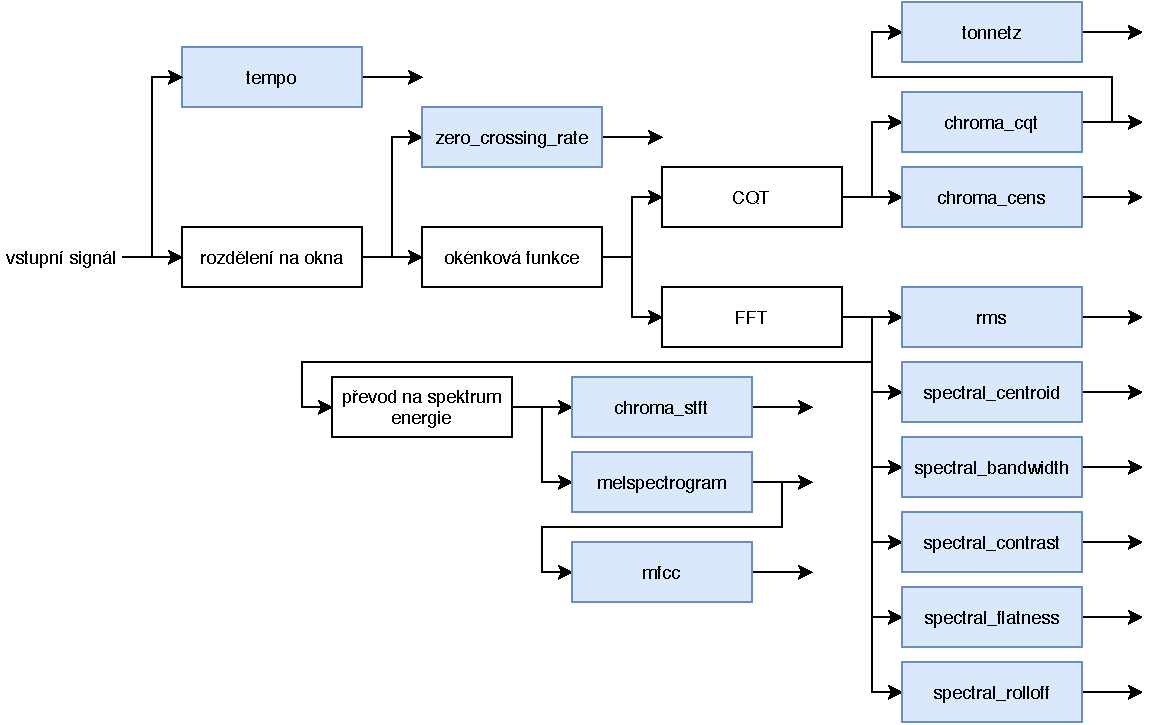
\includegraphics[width=\textwidth]{obrazky/librosa_extrakce.pdf}
    \caption{\textbf{Diagram průběhu extrakce atributů pomocí funkcí knihovny Librosa.} Z~načtené zvukové stopy je nejprve extrahován atribut \textit{tempo}, poté je stopa rozdělena na okna a je extrahován atribut \textit{zero crossing rate}. Dále je stopa vynásobena okénkovou funkcí a převedena do časově-frekvenční oblasti pomocí metody \textit{Constant-Q transform} nebo \textit{Short-time Fourier transform}. Pro některé z~atributů je toto frekvenční spektrum nakonec převedeno na spektrum energie. Následně je provedena extrakce ostatních atributů.}
    \label{obr_librosa_extrakce}
\end{figure*}


Knihovna Essentia umožňuje extrahovat všechny dostupné atributy pomocí jediné funkce. Protože však tato funkce nepodporuje načítání audio stop ve formátu \textit{ULAW}, u~datové sady GTZAN bylo nejprve nutné pomocí knihovny Soundfile skladby načíst a následně je dočasně uložit ve formátu \textit{WAVE}. Po zpracování byly konvertované skladby odstraněny. Funkce \textit{MusicExtractor} extrahuje ze skladby 49 nízkoúrovňových atributů, 14 atributů týkajících se rytmu a 17 atributů týkajících se melodie a harmonie. Podrobný popis této funkce, včetně všech jejích parametrů a extrahovaných atributů je možné nalézt v~oficiální dokumentaci knihovny Essentia.\footnote{\url{https://essentia.upf.edu/streaming\_extractor\_music.html}} 

Funkce \textit{MusicExtractor} vrací extrahované atributy ve dvou formách, a to v~neupravené podobě a po zpracování statistickými funkcemi. Pro následné zpracování byla opět kvůli příliš vysoké dimenzionalitě neupravených dat zvolena varianta druhá. Výchozí hodnoty parametrů extrakční funkce byly vyhodnoceny jako adekvátní a byly tak z~větší části ponechány beze změn. Rozšířen byl pouze počet použitých statistických funkcí za účelem zachování co největšího množství informací. Všechny zvolené hodnoty parametrů pro funkci \textit{MusicExtractor}, včetně jejich krátkého popisu, je možné vidět v~příloze~\ref{prilohy_k_extrakci_atributu}. Atributy extrahované pomocí knihovny Essentia tvoří celkem 4403 hodnot pro každou skladbu. Extrakce atributů pomocí knihovny Essentia trvala celkem 41 minut.

\subsection*{Selekce atributů}
\label{NIS_selekce_atributu}
Pro selekci atributů byly zvoleny dvě obalovací metody, a to \textit{dopředná selekce (forward selection, FS)} a \textit{zpětná eliminace (backward elimination, BE)}. Pro vyhodnocení úspěšnosti klasifikace byla z~důvodu příliš vysoké výpočetní náročnosti využita pouze validační sada. V~následujících podkapitolách jsou blíže popsány tyto metody a dosažené výsledky. Kvůli příliš vysokému počtu sad atributů a klasifikačních algoritmů nejsou vybrané atributy v~této práci zahrnuty. Lze je však dohledat na přiloženém médiu. Výpis průběhu selekce byl uložen do souboru \textit{feature\_selection.log} a samotné atributy pak do souboru \textit{optimised\_feature\_sets.json}.

\subsubsection*{Dopředná selekce}
\label{NIS_dopredna_selekce}
Počet atributů vybraných pomocí metody dopředné selekce je možné vidět v~tabulce~\ref{NIS_pocet_atributu_dopredna_selekce}. Ze 14 atributů extrahovaných pomocí knihovny Librosa byly vybrány průměrně 4 atributy a z~80 atributů extrahovaných pomocí knihovny Essentia pak 6 atributů. Pseudokód dopředné selekce je uveden v~algoritmu~\ref{pseudo_algoritmus_dopredne_selekce}. Selekce pomocí této metody trvala na všech sadách atributů celkem 14 hodin a 1 minutu. Informace o~délce běhu pro jednotlivé klasifikátory na každé ze sad atributů jsou uvedeny v~příloze~\ref{prilohy_k_selekci_atributu}.

\begin{algorithm}
    \caption{Pseudokód dopředné selekce}
    \label{pseudo_algoritmus_dopredne_selekce}
    \begin{algorithmic}[1]
        \State Zkopíruj všechny atributy do $remaining\_features[]$
        \State Nastav $max\_score$ na $0$
        \State Nastav $total\_max\_score$ na $0$
        \While {$i=0$ $<$ $len(features[])$}
            \For {$feature$ $in$ $remaining\_features[]$}
                \State Přidej $feature$ do $best\_features[]$
                \State Proveď klasifikaci na množině $best\_features[]$
                \If {$score > max\_score$}
                    \State Nastav $max\_score$ na $score$
                    \State Nastav $best\_feature$ na $feature$
                \EndIf
                \State Odstraň $feature$ z~$best\_features[]$
            \EndFor
            \If {$max\_score$ $<=$ $total\_max\_score$}
                \State Ukonči selekci
            \EndIf
            \State Nastav $total\_max\_score$ na $max\_score$
            \State Přidej $best\_feature$ do $best\_features[]$
            \State Odstraň $best\_feature$ z~$remaining\_features[]$
        \EndWhile
    \end{algorithmic}
\end{algorithm}

\begin{table}[H]
	\vskip6pt
    \caption{\textbf{Počet atributů vybraných pomocí metody dopředné selekce}}
    \label{NIS_pocet_atributu_dopredna_selekce}
    \vskip6pt
	\centering
    \resizebox{\textwidth}{!}{\begin{tabular}{llllllll}
                                                                        & \multicolumn{2}{l|}{EBD}                & \multicolumn{2}{l|}{FMA}                & \multicolumn{2}{l|}{GTZAN}              &                           \\
                                                                        & librosa & \multicolumn{1}{l|}{essentia} & librosa & \multicolumn{1}{l|}{essentia} & librosa & \multicolumn{1}{l|}{essentia} & \multirow{-2}{*}{Average} \\ \cline{2-8} 
    \multicolumn{1}{l|}{LogisticRegression}                             & 6       & 9                             & 7       & 11                            & 5       & 6                             & 7.$\overline{3}$          \\
    \rowcolor[HTML]{EFEFEF} 
    \multicolumn{1}{l|}{\cellcolor[HTML]{EFEFEF}KneighborsClassifier}   & 2       & 8                             & 3       & 8                             & 3       & 5                             & 4.8$\overline{3}$          \\
    \multicolumn{1}{l|}{MLPClassifier}                                  & 3       & 6                             & 6       & 2                             & 3       & 3                             & 3.8$\overline{3}$          \\
    \rowcolor[HTML]{EFEFEF} 
    \multicolumn{1}{l|}{\cellcolor[HTML]{EFEFEF}DecisionTreeClassifier} & 3       & 8                             & 5       & 6                             & 2       & 6                             & 5                         \\
    \multicolumn{1}{l|}{SVC\_linear}                                    & 4       & 4                             & 7       & 6                             & 2       & 4                             & 4.5                       \\
    \rowcolor[HTML]{EFEFEF} 
    \multicolumn{1}{l|}{\cellcolor[HTML]{EFEFEF}SVC\_rbf}               & 7       & 6                             & 4       & 15                            & 4       & 6                             & 7                         \\
    \multicolumn{1}{l|}{RandomForestClassifier}                         & 3       & 4                             & 3       & 6                             & 1       & 4                             & 3.5                       \\
    \rowcolor[HTML]{EFEFEF} 
    \multicolumn{1}{l|}{\cellcolor[HTML]{EFEFEF}XGBClassifier}          & 5       & 5                             & 4       & 4                             & 4       & 2                             & 4                         \\
    \multicolumn{1}{l|}{Average}                                        & 4.125   & 6.25                          & 4.875   & 7.25                          & 3       & 4.5                           & 5                        
    \end{tabular}}
\end{table}

\subsubsection*{Zpětná eliminace}
\label{NIS_zpetna_eliminace}
Počet atributů vybraných pomocí metody zpětné eliminace je možné vidět v~tabulce~\ref{NIS_pocet_atributu_zpetna_eliminace}. Ze 14 atributů extrahovaných pomocí knihovny Librosa bylo vybráno průměrně 10 atributů a z~80 atributů extrahovaných pomocí knihovny Essentia pak 67 atributů. Pseudokód zpětné eliminace je uveden v~algoritmu~\ref{pseudo_algoritmus_zpetne_eliminace}. Selekce pomocí této metody trvala na všech sadách atributů celkem 3 dny, 22 hodin a 53 minut. Informace o~délce běhu pro jednotlivé klasifikátory na každé ze sad atributů jsou uvedeny v~příloze~\ref{prilohy_k_selekci_atributu}.

\begin{algorithm}
    \caption{Pseudokód zpětné eliminace}
    \label{pseudo_algoritmus_zpetne_eliminace}
    \begin{algorithmic}[1]
        \State Zkopíruj všechny atributy do $best\_features[]$
        \State Proveď klasifikaci na množine $best\_features[]$
        \State Nastav $max\_score$ na $0$
        \State Nastav $total\_max\_score$ na $score$
        \While {$i=0$ $<$ $len(features[])$}
            \For {$feature$ $in$ $best\_features[]$}
                \State Odstraň $feature$ z~$best\_features[]$
                \State Proveď klasifikaci na množině $best\_features[]$
                \If {$score >= max\_score$}
                    \State Nastav $max\_score$ na $score$
                    \State Nastav $best\_feature$ na $feature$
                \EndIf
                \State Přidej $feature$ do $best\_features[]$
            \EndFor
            \If {$max\_score$ $<$ $total\_max\_score$}
                \State Ukonči selekci
            \EndIf
            \State Nastav $total\_max\_score$ na $max\_score$
            \State Nastav $max\_score$ na $0$
            \State Odstraň $best\_feature$ z~$best\_features[]$
        \EndWhile
    \end{algorithmic}
\end{algorithm}

\begin{table}[H]
    \vskip6pt
    \caption{\textbf{Počet atributů vybraných pomocí metody zpětné eliminace}}
    \label{NIS_pocet_atributu_zpetna_eliminace}
    \vskip6pt
    \centering
    \resizebox{\textwidth}{!}{\begin{tabular}{llllllll}
                                                                        & \multicolumn{2}{l|}{EBD}                & \multicolumn{2}{l|}{FMA}                & \multicolumn{2}{l|}{GTZAN}              &                           \\
                                                                        & librosa & \multicolumn{1}{l|}{essentia} & librosa & \multicolumn{1}{l|}{essentia} & librosa & \multicolumn{1}{l|}{essentia} & \multirow{-2}{*}{Average} \\ \cline{2-8} 
    \multicolumn{1}{l|}{LogisticRegression}                             & 12      & 48                            & 7       & 73                            & 12      & 37                            & 31.5                      \\
    \rowcolor[HTML]{EFEFEF} 
    \multicolumn{1}{l|}{\cellcolor[HTML]{EFEFEF}KneighborsClassifier}   & 7       & 66                            & 12      & 73                            & 8       & 72                            & 39.$\overline{6}$          \\
    \multicolumn{1}{l|}{MLPClassifier}                                  & 10      & 80                            & 13      & 79                            & 11      & 80                            & 45.5                      \\
    \rowcolor[HTML]{EFEFEF} 
    \multicolumn{1}{l|}{\cellcolor[HTML]{EFEFEF}DecisionTreeClassifier} & 13      & 75                            & 12      & 80                            & 10      & 79                            & 44.8$\overline{3}$          \\
    \multicolumn{1}{l|}{SVC\_linear}                                    & 11      & 58                            & 12      & 75                            & 9       & 26                            & 31.8$\overline{3}$          \\
    \rowcolor[HTML]{EFEFEF} 
    \multicolumn{1}{l|}{\cellcolor[HTML]{EFEFEF}SVC\_rbf}               & 7       & 47                            & 8       & 67                            & 6       & 51                            & 31                        \\
    \multicolumn{1}{l|}{RandomForestClassifier}                         & 12      & 76                            & 13      & 79                            & 12      & 75                            & 44.5                      \\
    \rowcolor[HTML]{EFEFEF} 
    \multicolumn{1}{l|}{\cellcolor[HTML]{EFEFEF}XGBClassifier}          & 9       & 76                            & 13      & 78                            & 13      & 62                            & 41.8$\overline{3}$          \\
    \multicolumn{1}{l|}{Average}                                        & 10.125  & 65.75                         & 11.25   & 75.5                          & 10.125  & 60.25                         & 38.8$\overline{3}$         
    \end{tabular}}
\end{table}

\subsubsection*{Zhodnocení výsledků selekece atributů}
\label{NIS_zhodnoceni_vysledku_selekce_atributu}
Vliv selekce atributů na skóre jednotlivých klasifikátorů na validačních sadách je možné vidět v~tabulce~\ref{tabulka_selekce_atributu_librosa_skore} pro atributy extrahované pomocí knihovny Librosa a v~tabulce~\ref{tabulka_selekce_atributu_essentia_skore} pro atributy extrahované pomocí knihovny Essentia. Vliv na dobu trénování a klasifikace pak v~příloze~\ref{prilohy_k_selekci_atributu}. Z~výsledků je patrné, že skóre na podmnožině atributů získané pomocí metody dopředné selekce bylo v~drtivé většině vyšší, než na celé množině atributů. Na atributech extrahovaných pomocí knihovny Librosa bylo dosaženo zvýšení skóre ve všech případech, na atributech extrahovaných pomocí knihovny Essentia pak už jen v~devatenácti ze čtyřiadvaceti případů. Pomocí metody zpětné eliminace pak bylo dosaženo zvýšení skóre ve všech případech. Jelikož však ve spoustě případů pomocí metody dopředné selekce bylo dosaženo vyššího nárůstu skóre, než pomocí metody zpětné eliminace, nelze prohlásit, že by metoda zpětné eliminace byla obecně lepší. Z~toho důvodu byly pro následnou optimalizaci parametrů využity podmnožiny atributů získané pomocí obou metod.

Dále je také nutné podotknout, že testování úspěšnosti klasifikace bylo prováděno na stejné validační sadě, na jaké byla testována úspěšnost při samotné selekci atributů. Dá se tedy předpokládat, že výsledky klasifikace na sadě testovací budou odlišné. V~neposlední řadě je z~výsledků klasifikace patrné, že na sadách atributů extrahovaných pomocí knihovny Essentia bylo obecně dosaženo vyššího skóre, než na sadách atributů extrahovaných pomocí knihovny Librosa. Jediným případem, kdy nejvyššího skóre bylo dosaženo pomocí atributů knihovny Librosa, je klasifikátor \textit{MLPClassifier} na datové sadě GTZAN. Z~toho důvodu byly atributy extrahované pomocí knihovny Librosa vyhodnoceny jako nedostatečné, a pro následnou optimalizaci parametrů a klasifikaci byly využity pouze atributy extrahované pomocí knihovny Essentia.

\begin{table}[H]
	\vskip6pt
    \caption{\textbf{Rozdíl skóre po selekci atributů extrahovaných pomocí knihovny Librosa na validační sadě}}
    \label{tabulka_selekce_atributu_librosa_skore}  
    \vskip6pt
	\centering
    \resizebox{\textwidth}{!}{\begin{tabular}{lllllllllll}
                              &                                                 & LR                             & KNNC                           & MLPC                           & DTC                            & SCVL                           & SVCR                            & RFC                             & XGBC                           & Average                        \\ \cline{3-11} 
                              & \multicolumn{1}{l|}{FS}                         & 3.44\%                         & 14.50\%                        & 6.88\%                         & 1.94\%                         & 0.45\%                         & 8.52\%                          & 10.16\%                         & 0.45\%                         & 5.79\%                         \\
    \multirow{-2}{*}{EBD}     & \multicolumn{1}{l|}{\cellcolor[HTML]{EFEFEF}BE} & \cellcolor[HTML]{EFEFEF}1.35\% & \cellcolor[HTML]{EFEFEF}8.22\% & \cellcolor[HTML]{EFEFEF}5.38\% & \cellcolor[HTML]{EFEFEF}2.24\% & \cellcolor[HTML]{EFEFEF}2.84\% & \cellcolor[HTML]{EFEFEF}8.52\%  & \cellcolor[HTML]{EFEFEF}6.43\%  & \cellcolor[HTML]{EFEFEF}2.24\% & \cellcolor[HTML]{EFEFEF}4.65\% \\ \cline{1-2}
                              & \multicolumn{1}{l|}{FS}                         & 8.98\%                         & 4.06\%                         & 0.47\%                         & 2.11\%                         & 4.45\%                         & 2.34\%                          & 0.94\%                          & 1.25\%                         & 3.08\%                         \\
    \multirow{-2}{*}{FMA}     & \multicolumn{1}{l|}{\cellcolor[HTML]{EFEFEF}BE} & \cellcolor[HTML]{EFEFEF}8.98\% & \cellcolor[HTML]{EFEFEF}3.20\% & \cellcolor[HTML]{EFEFEF}1.41\% & \cellcolor[HTML]{EFEFEF}1.80\% & \cellcolor[HTML]{EFEFEF}0.86\% & \cellcolor[HTML]{EFEFEF}3.44\%  & \cellcolor[HTML]{EFEFEF}0.70\%  & \cellcolor[HTML]{EFEFEF}2.27\% & \cellcolor[HTML]{EFEFEF}2.83\% \\ \cline{1-2}
                              & \multicolumn{1}{l|}{FS}                         & 4.38\%                         & 6.25\%                         & 5.00\%                         & 5.00\%                         & 3.75\%                         & 16.88\%                         & 12.50\%                         & 3.75\%                         & 7.19\%                         \\
    \multirow{-2}{*}{GTZAN}   & \multicolumn{1}{l|}{\cellcolor[HTML]{EFEFEF}BE} & \cellcolor[HTML]{EFEFEF}7.50\% & \cellcolor[HTML]{EFEFEF}0.62\% & \cellcolor[HTML]{EFEFEF}7.50\% & \cellcolor[HTML]{EFEFEF}7.50\% & \cellcolor[HTML]{EFEFEF}7.50\% & \cellcolor[HTML]{EFEFEF}16.25\% & \cellcolor[HTML]{EFEFEF}11.25\% & \cellcolor[HTML]{EFEFEF}1.88\% & \cellcolor[HTML]{EFEFEF}7.50\% \\ \cline{1-2}
                              & \multicolumn{1}{l|}{FS}                         & 5.60\%                         & 8.27\%                         & 4.12\%                         & 3.02\%                         & 2.88\%                         & 9.25\%                          & 7.87\%                          & 1.82\%                         & 5.35\%                         \\
    \multirow{-2}{*}{Average} & \multicolumn{1}{l|}{\cellcolor[HTML]{EFEFEF}BE} & \cellcolor[HTML]{EFEFEF}5.94\% & \cellcolor[HTML]{EFEFEF}4.01\% & \cellcolor[HTML]{EFEFEF}4.76\% & \cellcolor[HTML]{EFEFEF}3.85\% & \cellcolor[HTML]{EFEFEF}3.73\% & \cellcolor[HTML]{EFEFEF}9.40\%  & \cellcolor[HTML]{EFEFEF}6.13\%  & \cellcolor[HTML]{EFEFEF}2.13\% & \cellcolor[HTML]{EFEFEF}5.00\%
    \end{tabular}}
\end{table}

\begin{table}[H]
	\vskip6pt
    \caption{\textbf{Rozdíl skóre po selekci atributů extrahovaných pomocí knihovny Essentia na validační sadě}}
    \label{tabulka_selekce_atributu_essentia_skore}  
    \vskip6pt
	\centering
    \resizebox{\textwidth}{!}{\begin{tabular}{lllllllllll}
                              &                                                 & LR                             & KNNC                            & MLPC                           & DTC                            & SCVL                           & SVCR                            & RFC                            & XGBC                           & Average                        \\ \cline{3-11} 
                              & \multicolumn{1}{l|}{FS}                         & 0.75\%                         & 30.64\%                         & 8.07\%                         & 10.31\%                        & -2.69\%                        & 10.61\%                         & 3.59\%                         & 0.90\%                         & 7.77\%                         \\
    \multirow{-2}{*}{EBD}     & \multicolumn{1}{l|}{\cellcolor[HTML]{EFEFEF}BE} & \cellcolor[HTML]{EFEFEF}3.74\% & \cellcolor[HTML]{EFEFEF}14.20\% & \cellcolor[HTML]{EFEFEF}4.19\% & \cellcolor[HTML]{EFEFEF}6.58\% & \cellcolor[HTML]{EFEFEF}1.49\% & \cellcolor[HTML]{EFEFEF}13.75\% & \cellcolor[HTML]{EFEFEF}2.39\% & \cellcolor[HTML]{EFEFEF}2.09\% & \cellcolor[HTML]{EFEFEF}6.05\% \\ \cline{1-2}
                              & \multicolumn{1}{l|}{FS}                         & 10.70\%                        & 6.17\%                          & -4.61\%                        & 2.42\%                         & 6.33\%                         & 5.47\%                          & 0.62\%                         & 0.94\%                         & 3.51\%                         \\
    \multirow{-2}{*}{FMA}     & \multicolumn{1}{l|}{\cellcolor[HTML]{EFEFEF}BE} & \cellcolor[HTML]{EFEFEF}3.52\% & \cellcolor[HTML]{EFEFEF}1.33\%  & \cellcolor[HTML]{EFEFEF}2.03\% & \cellcolor[HTML]{EFEFEF}4.22\% & \cellcolor[HTML]{EFEFEF}2.34\% & \cellcolor[HTML]{EFEFEF}3.05\%  & \cellcolor[HTML]{EFEFEF}1.17\% & \cellcolor[HTML]{EFEFEF}3.28\% & \cellcolor[HTML]{EFEFEF}2.62\% \\ \cline{1-2}
                              & \multicolumn{1}{l|}{FS}                         & 0.00\%                         & 13.75\%                         & 5.63\%                         & 6.88\%                         & -1.25\%                        & 7.50\%                          & 3.13\%                         & -3.12\%                        & 4.07\%                         \\
    \multirow{-2}{*}{GTZAN}   & \multicolumn{1}{l|}{\cellcolor[HTML]{EFEFEF}BE} & \cellcolor[HTML]{EFEFEF}3.75\% & \cellcolor[HTML]{EFEFEF}15.00\% & \cellcolor[HTML]{EFEFEF}5.00\% & \cellcolor[HTML]{EFEFEF}6.88\% & \cellcolor[HTML]{EFEFEF}4.38\% & \cellcolor[HTML]{EFEFEF}6.88\%  & \cellcolor[HTML]{EFEFEF}5.00\% & \cellcolor[HTML]{EFEFEF}3.75\% & \cellcolor[HTML]{EFEFEF}6.33\% \\ \cline{1-2}
                              & \multicolumn{1}{l|}{FS}                         & 3.82\%                         & 16.85\%                         & 3.03\%                         & 6.54\%                         & 0.80\%                         & 7.86\%                          & 2.45\%                         & -0.43\%                        & 5.11\%                         \\
    \multirow{-2}{*}{Average} & \multicolumn{1}{l|}{\cellcolor[HTML]{EFEFEF}BE} & \cellcolor[HTML]{EFEFEF}3.67\% & \cellcolor[HTML]{EFEFEF}10.18\% & \cellcolor[HTML]{EFEFEF}3.74\% & \cellcolor[HTML]{EFEFEF}5.89\% & \cellcolor[HTML]{EFEFEF}2.74\% & \cellcolor[HTML]{EFEFEF}7.89\%  & \cellcolor[HTML]{EFEFEF}2.85\% & \cellcolor[HTML]{EFEFEF}3.04\% & \cellcolor[HTML]{EFEFEF}5.00\%
    \end{tabular}}
\end{table}

\section{Optimalizace parametrů klasifikačních algoritmů}
\label{NIS_optimalizace_paramteru_klasifikacnich_algoritmu}
Pro optimalizaci parametrů klasifikátorů byla využita knihovna Optuna (verze~1.5.0). Tato knihovna je implementována v~jazyce Python a obsahuje několik algoritmů pro vyhledání optimálních hodnot parametrů. Za účelem optimalizace byla vytvořena třída \textit{HPoptimise} obsahující optimalizační funkce pro každý z~klasifikačních algoritmů využitých v~této práci. parametry každého z~osmi použitých klasifikátorů byly následně optimalizovány pomocí jednoho ze dvou vybraných optimalizačních algoritmů.

Prvním z~nich je algoritmus \textit{GridSampler}, který metodou \textit{vyčerpávajícího hledání (exhaustive search)} prohledává předem definovaný prostor parametrů. Tato metoda tedy vyzkouší každou z~možných kombinací parametrů z~definovaného prostoru, a je tak vždy schopna nalézt optimální řešení. Její nevýhodou je však vysoká výpočetní náročnost, a je tak vhodné ji využít pouze v~případě, kdy prostor parametrů není příliš obsáhlý, či samotný klasifikační algoritmus je velmi málo výpočetně náročný. Tento algoritmus byl využit pro optimalizaci parametrů klasifikátorů \textit{LogisticRegression}, \textit{KNeighborsClassifier}, \textit{SVC\_linear} a \textit{SVC\_rbf}.

Druhým algoritmem je \textit{Tree-structured Parzen Estimator (TPE)}, který nejprve provádí náhodný výběr parametrů z~definovaného prostoru a následně na základě výsledků klasifikace vybírá takové kombinace parametrů, na nichž bylo v~předešlých iteracích dosaženo nejlepších výsledků. Tímto způsobem je tak algoritmus schopen konvergovat k~optimálnímu řešení a je tak vhodný i pro rozsáhlejší prostory parametrů, či výpočetně náročnější klasifikační algoritmy. Jeho nevýhodou však je, že v~případě, kdy v~prvních iteracích s~náhodným výběrem nejsou zvoleny vhodné kombinace parametrů, může konvergovat k~řešení, které je pouze lokálně optimální. Tento algoritmus byl využit pro optimalizaci parametrů klasifikátorů \textit{MLPClassifier}, \textit{DecisionTreeClassifier}, \textit{RandomForestClassifier} a \textit{XGBClassifier}.

Stejně jako u~selekce atributů byla z~důvodu příliš vysoké výpočetní náročnosti úspěšnost vybraných parametrů testována pomocí validační sady. Samotné prostory parametrů byly zvoleny pomocí řady experimentů na různých kombinacích parametrů, které byly, na základě oficiálních dokumentací knihoven obsahující využité klasifikační algoritmy, vyhodnoceny jako potenciálně blízké hodnotám optimálním. Optimalizace pomocí algoritmu \textit{TPE} byla ukončena vždy, když proběhlo sto iterací, při kterých nebylo dosaženo navýšení skóre. U~obou algoritmů pak na konci každé iterace byly uloženy dosavadní výsledky a také vypsány aktuální informace o~stavu optimalizace. Optimalizované parametry byly uloženy do souboru souboru \textit{optimised\_hyper\_parameters.json}. Optimalizace parametrů všech klasifikátorů na všech sadách atributů trvala celkem 3 dny, 19 hodin a 19 minut.  Informace o~délce běhu pro jednotlivé klasifikátory na každé ze sad atributů jsou uvedeny v~příloze~\ref{prilohy_k_optimalizaci_parametru}. Všechny parametry, jejichž hodnoty byly optimalizovány, je možné vidět v~následujícím seznamu.

\begin{itemize}
    \item LogisticRegression (LR) - \textit{penalty}, \textit{fit\_intercept}, \textit{C}
    \item KNearestNeighbors (KNNC) - \textit{n\_neighbors}, \textit{weights}, \textit{p}
    \item MLPClassifier (MLPC) - \textit{solver}, \textit{hidden\_layer\_sizes}, \textit{activation}, \textit{alpha}, \textit{momentum}, \textit{epsilon}
    \item DecisionTreeClassifier (DTC) - \textit{criterion}, \textit{min\_samples\_split}, \textit{min\_samples\_leaf},
    \newline \textit{max\_features}, \textit{ccp\_alpha}
    \item SVC\_linear (SVCL) - \textit{C}
    \item SVC\_rbf (SVCR) - \textit{C}, \textit{gamma}
    \item RandomForestClassifier (RFC) - \textit{criterion}, \textit{min\_samples\_split}, \textit{min\_samples\_leaf}, \textit{max\_features}, \textit{ccp\_alpha}, \textit{max\_samples}
    \item XGBClassifier (XGBC) - \textit{n\_estimators}, \textit{max\_depth}, \textit{min\_child\_weight}, \textit{subsample}, \textit{colsample\_bytree}, \textit{reg\_alpha}, \textit{reg\_lambda}, \textit{gamma}
\end{itemize}

\subsubsection*{Zhodnocení výsledků optimalizace parametrů}
\label{NIS_zhodnoceni_vysledku_optimalizace_parametru}

Vliv optimalizace parametrů na skóre na validačních sadách je možné vidět v~tabulce~\ref{tabulka_optimalizace_parametru_skore} a vliv na dobu trénování a klasifikace pak v~příloze~\ref{prilohy_ke_klasifikaci_a_zhodnoceni_vysledku}. Průměrné zvýšení skóre na množině všech atributů dosahovalo 5 \%, což je velmi podobný výsledek, jakého bylo dosaženo pomocí metod selekce atributů. Na samotných podmnožinách atributů však optimalizace parametrů dosahovala mnohem nižšího nárůstu skóre, kdy na podmnožině získané metodou dopředné selekce nárůst skóre dosahoval pouze 0.32 \% a na podmnožině získané metodou zpětné eliminace 1.35 \%. Tento výsledek je možné vysvětlit tím, že vyhodnocení u~selekce atributů bylo prováděno pomocí klasifikátorů s~výchozími hodnotami parametrů. Vybrané podmnožiny tak byly ideální pro tyto hodnoty parametrů a jejich následná optimalizace již nebyla tak přínosná.

\begin{table}[H]
	\vskip6pt
    \caption{\textbf{Rozdíl skóre klasifikace po optimalizaci parametrů na validační sadě}}
    \label{tabulka_optimalizace_parametru_skore}  
    \vskip6pt
	\centering
    \resizebox{\textwidth}{!}{\begin{tabular}{lllllllllll}
                              &                                                  & LR                             & KNNC                           & MLPC                           & DTC                             & SVCL                           & SVCR                           & RFC                             & XGBC                           & Average                         \\ \cline{3-11} 
                              & \multicolumn{1}{l|}{All}                         & 0.15\%                         & 11.06\%                        & 8.82\%                         & 4.19\%                          & 0.00\%                         & 11.06\%                        & 4.04\%                          & 2.54\%                         & 5.23\%                          \\
                              & \multicolumn{1}{l|}{\cellcolor[HTML]{EFEFEF}FS}  & \cellcolor[HTML]{EFEFEF}0.15\% & \cellcolor[HTML]{EFEFEF}0.00\% & \cellcolor[HTML]{EFEFEF}0.00\% & \cellcolor[HTML]{EFEFEF}0.45\%  & \cellcolor[HTML]{EFEFEF}0.00\% & \cellcolor[HTML]{EFEFEF}0.30\% & \cellcolor[HTML]{EFEFEF}0.00\%  & \cellcolor[HTML]{EFEFEF}0.00\% & \cellcolor[HTML]{EFEFEF}0.11\%  \\
    \multirow{-3}{*}{EBD}     & \multicolumn{1}{l|}{BE}                          & 0.00\%                         & 5.23\%                         & 4.63\%                         & 0.60\%                          & 0.00\%                         & 0.00\%                         & 1.20\%                          & 0.75\%                         & 1.55\%                          \\ \cline{1-2}
                              & \multicolumn{1}{l|}{\cellcolor[HTML]{EFEFEF}All} & \cellcolor[HTML]{EFEFEF}8.52\% & \cellcolor[HTML]{EFEFEF}3.98\% & \cellcolor[HTML]{EFEFEF}4.77\% & \cellcolor[HTML]{EFEFEF}7.42\%  & \cellcolor[HTML]{EFEFEF}6.80\% & \cellcolor[HTML]{EFEFEF}2.27\% & \cellcolor[HTML]{EFEFEF}0.86\%  & \cellcolor[HTML]{EFEFEF}4.30\% & \cellcolor[HTML]{EFEFEF}4.87\%  \\
                              & \multicolumn{1}{l|}{FS}                          & 0.00\%                         & 0.55\%                         & 1.25\%                         & 5.39\%                          & 0.00\%                         & 0.00\%                         & -0.70\%                         & 2.19\%                         & 1.09\%                          \\
    \multirow{-3}{*}{FMA}     & \multicolumn{1}{l|}{\cellcolor[HTML]{EFEFEF}BE}  & \cellcolor[HTML]{EFEFEF}5.23\% & \cellcolor[HTML]{EFEFEF}2.58\% & \cellcolor[HTML]{EFEFEF}1.56\% & \cellcolor[HTML]{EFEFEF}3.20\%  & \cellcolor[HTML]{EFEFEF}3.83\% & \cellcolor[HTML]{EFEFEF}0.00\% & \cellcolor[HTML]{EFEFEF}-0.23\% & \cellcolor[HTML]{EFEFEF}0.78\% & \cellcolor[HTML]{EFEFEF}2.12\%  \\ \cline{1-2}
                              & \multicolumn{1}{l|}{All}                         & 0.00\%                         & 11.88\%                        & 8.75\%                         & 5.63\%                          & 0.00\%                         & 6.25\%                         & 3.75\%                          & 5.00\%                         & 5.16\%                          \\
                              & \multicolumn{1}{l|}{\cellcolor[HTML]{EFEFEF}FS}  & \cellcolor[HTML]{EFEFEF}0.00\% & \cellcolor[HTML]{EFEFEF}1.25\% & \cellcolor[HTML]{EFEFEF}1.25\% & \cellcolor[HTML]{EFEFEF}-4.38\% & \cellcolor[HTML]{EFEFEF}0.00\% & \cellcolor[HTML]{EFEFEF}0.00\% & \cellcolor[HTML]{EFEFEF}-1.88\% & \cellcolor[HTML]{EFEFEF}1.88\% & \cellcolor[HTML]{EFEFEF}-0.24\% \\
    \multirow{-3}{*}{GTZAN}   & \multicolumn{1}{l|}{BE}                          & 0.00\%                         & 1.88\%                         & 3.75\%                         & -1.88\%                         & 0.00\%                         & 0.62\%                         & -3.13\%                         & 1.88\%                         & 0.39\%                          \\ \cline{1-2}
                              & \multicolumn{1}{l|}{\cellcolor[HTML]{EFEFEF}All} & \cellcolor[HTML]{EFEFEF}2.89\% & \cellcolor[HTML]{EFEFEF}8.97\% & \cellcolor[HTML]{EFEFEF}7.45\% & \cellcolor[HTML]{EFEFEF}5.75\%  & \cellcolor[HTML]{EFEFEF}2.27\% & \cellcolor[HTML]{EFEFEF}6.53\% & \cellcolor[HTML]{EFEFEF}2.88\%  & \cellcolor[HTML]{EFEFEF}3.95\% & \cellcolor[HTML]{EFEFEF}5.09\%  \\
                              & \multicolumn{1}{l|}{FS}                          & 0.05\%                         & 0.60\%                         & 0.83\%                         & 0.49\%                          & 0.00\%                         & 0.10\%                         & -0.86\%                         & 1.36\%                         & 0.32\%                          \\
    \multirow{-3}{*}{Average} & \multicolumn{1}{l|}{\cellcolor[HTML]{EFEFEF}BE}  & \cellcolor[HTML]{EFEFEF}1.74\% & \cellcolor[HTML]{EFEFEF}3.23\% & \cellcolor[HTML]{EFEFEF}3.31\% & \cellcolor[HTML]{EFEFEF}0.64\%  & \cellcolor[HTML]{EFEFEF}1.28\% & \cellcolor[HTML]{EFEFEF}0.21\% & \cellcolor[HTML]{EFEFEF}-0.72\% & \cellcolor[HTML]{EFEFEF}1.14\% & \cellcolor[HTML]{EFEFEF}1.35\% 
    \end{tabular}}
\end{table}

\begin{figure*}[h]
    \centering
    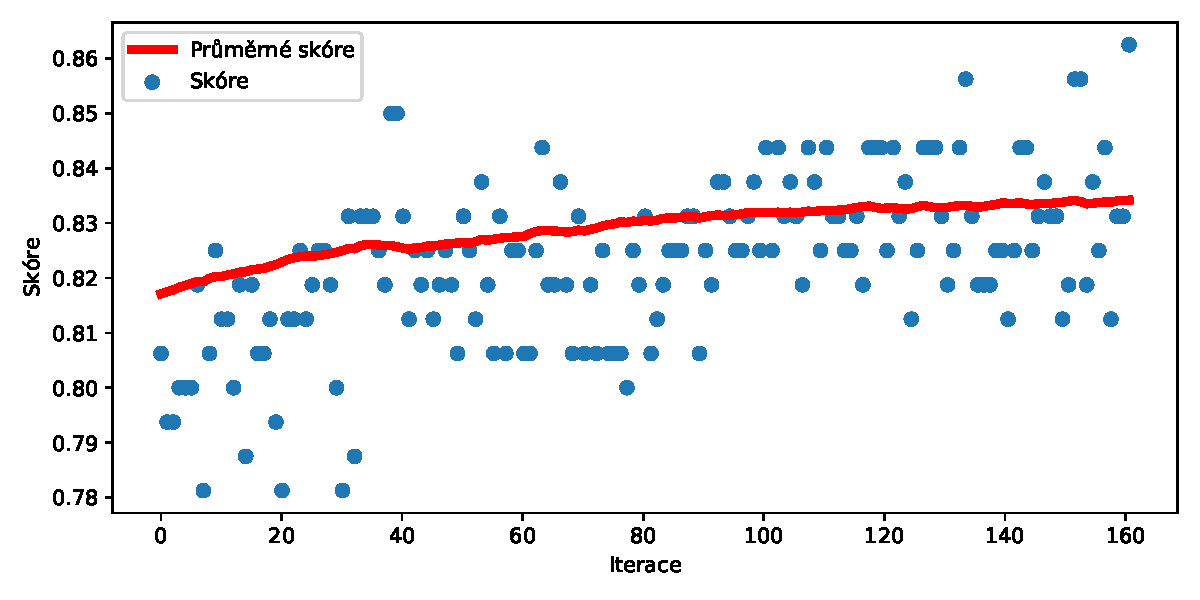
\includegraphics[width=\textwidth]{obrazky/TPESampler_optimisation.pdf}
    \caption{\textbf{Ukázka průběhu optimalizace parametrů pomocí algoritmu \textit{TPESampler}.} V~obrázku je možné vidět průběh optimalizace klasifikátoru \textit{XGBClassifier} na datové sadě GTZAN až po nejlepší iteraci. Červená čára značí průměrné skóre sta následujících iterací. Z~obrázku je patrný postupný nárůst skóre, jak optimalizační algoritmus konverguje k~optimálním hodnotám parametrů.}
    \label{obr_TPE_optimalizace}
\end{figure*}

\chapter{Klasifikace a zhodnocení výsledků}
\label{klasifikace_a_zhodnoceni_vysledku}

Úspěšnost selekce atributů na testovacích sadách je možné vidět v~tabulce~\ref{tabulka_selekce_atributu_zlepseni_testovaci_sada}. Z~výsledků je patrné, že na testovacích sadách selekce atributů nedosáhla zdaleka tak vysokého nárůstu úspěšnosti klasifikace, jako na sadách validačních. Na podmnožině atributů získaných pomocí metody dopředné selekce bylo dokonce průměrné skóre o~0.36 \% nižší, než na celé množině atributů. Na podmnožině získané pomocí metody zpětné eliminace pak bylo průměrně skóre o~1.09 \% vyšší. Toto dramatické snížení úspěšnosti klasifikace na testovací sadě je pravděpodobně způsobeno nedostatečnou velikostí datových sad a také použitím validace na jediné sadě, namísto křížové validace na několika sadách. 

\begin{table}[H]
	\vskip6pt
    \caption{\textbf{Rozdíl skóre klasifikace po selekci atributů na testovací sadě}}
    \label{tabulka_selekce_atributu_zlepseni_testovaci_sada}  
    \vskip6pt
	\centering
    \resizebox{\textwidth}{!}{\begin{tabular}{lllllllllll}
                              &                                                 & LR                              & KNNC                           & MLPC                            & DTC                             & SCVL                            & SVCR                           & RFC                            & XGBC                           & Average                         \\ \cline{3-11} 
                              & \multicolumn{1}{l|}{FS}                         & -3.11\%                         & 25.00\%                        & 1.79\%                          & -2.75\%                         & -4.07\%                         & 4.78\%                         & 3.11\%                         & -2.99\%                        & 2.72\%                          \\
    \multirow{-2}{*}{EBD}     & \multicolumn{1}{l|}{\cellcolor[HTML]{EFEFEF}BE} & \cellcolor[HTML]{EFEFEF}0.12\%  & \cellcolor[HTML]{EFEFEF}9.45\% & \cellcolor[HTML]{EFEFEF}-0.24\% & \cellcolor[HTML]{EFEFEF}-1.20\% & \cellcolor[HTML]{EFEFEF}-0.36\% & \cellcolor[HTML]{EFEFEF}6.22\% & \cellcolor[HTML]{EFEFEF}1.79\% & \cellcolor[HTML]{EFEFEF}0.24\% & \cellcolor[HTML]{EFEFEF}2.00\%  \\ \cline{1-2}
                              & \multicolumn{1}{l|}{FS}                         & 4.06\%                          & 1.88\%                         & -0.75\%                         & -1.31\%                         & 2.25\%                          & 1.38\%                         & -1.13\%                        & -2.19\%                        & 0.52\%                          \\
    \multirow{-2}{*}{FMA}     & \multicolumn{1}{l|}{\cellcolor[HTML]{EFEFEF}BE} & \cellcolor[HTML]{EFEFEF}-0.13\% & \cellcolor[HTML]{EFEFEF}0.12\% & \cellcolor[HTML]{EFEFEF}6.50\%  & \cellcolor[HTML]{EFEFEF}2.63\%  & \cellcolor[HTML]{EFEFEF}-0.75\% & \cellcolor[HTML]{EFEFEF}1.50\% & \cellcolor[HTML]{EFEFEF}0.75\% & \cellcolor[HTML]{EFEFEF}0.62\% & \cellcolor[HTML]{EFEFEF}1.41\%  \\ \cline{1-2}
                              & \multicolumn{1}{l|}{FS}                         & -5.00\%                         & -1.50\%                        & -2.00\%                         & -6.50\%                         & -7.00\%                         & 2.00\%                         & -9.00\%                        & -5.50\%                        & -4.31\%                         \\
    \multirow{-2}{*}{GTZAN}   & \multicolumn{1}{l|}{\cellcolor[HTML]{EFEFEF}BE} & \cellcolor[HTML]{EFEFEF}-1.00\% & \cellcolor[HTML]{EFEFEF}0.50\% & \cellcolor[HTML]{EFEFEF}-1.00\% & \cellcolor[HTML]{EFEFEF}-3.50\% & \cellcolor[HTML]{EFEFEF}-0.50\% & \cellcolor[HTML]{EFEFEF}3.00\% & \cellcolor[HTML]{EFEFEF}0.50\% & \cellcolor[HTML]{EFEFEF}1.00\% & \cellcolor[HTML]{EFEFEF}-0.13\% \\ \cline{1-2}
                              & \multicolumn{1}{l|}{FS}                         & -1.35\%                         & 8.46\%                         & -0.32\%                         & -3.52\%                         & -2.94\%                         & 2.72\%                         & -2.34\%                        & -3.56\%                        & -0.36\%                         \\
    \multirow{-2}{*}{Average} & \multicolumn{1}{l|}{\cellcolor[HTML]{EFEFEF}BE} & \cellcolor[HTML]{EFEFEF}-0.34\% & \cellcolor[HTML]{EFEFEF}3.36\% & \cellcolor[HTML]{EFEFEF}1.75\%  & \cellcolor[HTML]{EFEFEF}-0.69\% & \cellcolor[HTML]{EFEFEF}-0.54\% & \cellcolor[HTML]{EFEFEF}3.57\% & \cellcolor[HTML]{EFEFEF}1.01\% & \cellcolor[HTML]{EFEFEF}0.62\% & \cellcolor[HTML]{EFEFEF}1.09\% 
    \end{tabular}}
\end{table}

Úspěšnost optimalizace parametrů na testovacích sadách je možné vidět v~tabulce~\ref{tabulka_optimalizace_parametru_zlepseni_testovaci_sada}. V~porovnání se selekcí atributů byla úspěšnost optimalizace na testovací sadě výrazně vyšší. Průměrný nárůst skóre činil 2.83 \% na celé množině atributů, 0.78 \% na podmnožině získané pomocí metod dopředné selekce a 2.28 \% na podmnožině získané pomocí metody zpětné eliminace. 

\begin{table}[H]
	\vskip6pt
    \caption{\textbf{Rozdíl skóre klasifikace po optimalizaci parametrů na testovací sadě}}
    \label{tabulka_optimalizace_parametru_zlepseni_testovaci_sada}  
    \vskip6pt
	\centering
    \resizebox{\textwidth}{!}{\begin{tabular}{lllllllllll}
                              &                                                  & LR                             & KNNC                           & MLPC                            & DTC                            & SVCL                           & SVCR                           & RFC                             & XGBC                            & Average                        \\ \cline{3-11} 
                              & \multicolumn{1}{l|}{All}                         & -0.48\%                        & 7.89\%                         & 2.63\%                          & -0.36\%                        & 0.00\%                         & 7.18\%                         & 2.39\%                          & 0.12\%                          & 2.42\%                         \\
                              & \multicolumn{1}{l|}{\cellcolor[HTML]{EFEFEF}FS}  & \cellcolor[HTML]{EFEFEF}1.56\% & \cellcolor[HTML]{EFEFEF}0.00\% & \cellcolor[HTML]{EFEFEF}0.12\%  & \cellcolor[HTML]{EFEFEF}3.11\% & \cellcolor[HTML]{EFEFEF}0.00\% & \cellcolor[HTML]{EFEFEF}1.67\% & \cellcolor[HTML]{EFEFEF}-0.36\% & \cellcolor[HTML]{EFEFEF}1.08\%  & \cellcolor[HTML]{EFEFEF}0.90\% \\
    \multirow{-3}{*}{EBD}     & \multicolumn{1}{l|}{BE}                          & 0.00\%                         & 7.89\%                         & 1.91\%                          & 1.91\%                         & 0.12\%                         & 0.00\%                         & 2.51\%                          & -0.36\%                         & 1.75\%                         \\ \cline{1-2}
                              & \multicolumn{1}{l|}{\cellcolor[HTML]{EFEFEF}All} & \cellcolor[HTML]{EFEFEF}6.38\% & \cellcolor[HTML]{EFEFEF}4.31\% & \cellcolor[HTML]{EFEFEF}12.00\% & \cellcolor[HTML]{EFEFEF}5.75\% & \cellcolor[HTML]{EFEFEF}7.13\% & \cellcolor[HTML]{EFEFEF}1.94\% & \cellcolor[HTML]{EFEFEF}0.44\%  & \cellcolor[HTML]{EFEFEF}1.69\%  & \cellcolor[HTML]{EFEFEF}4.96\% \\
                              & \multicolumn{1}{l|}{FS}                          & 0.00\%                         & 0.56\%                         & 4.75\%                          & 4.50\%                         & 0.00\%                         & 0.00\%                         & 0.06\%                          & 1.25\%                          & 1.39\%                         \\
    \multirow{-3}{*}{FMA}     & \multicolumn{1}{l|}{\cellcolor[HTML]{EFEFEF}BE}  & \cellcolor[HTML]{EFEFEF}5.44\% & \cellcolor[HTML]{EFEFEF}4.75\% & \cellcolor[HTML]{EFEFEF}4.31\%  & \cellcolor[HTML]{EFEFEF}3.13\% & \cellcolor[HTML]{EFEFEF}6.69\% & \cellcolor[HTML]{EFEFEF}0.00\% & \cellcolor[HTML]{EFEFEF}0.31\%  & \cellcolor[HTML]{EFEFEF}0.69\%  & \cellcolor[HTML]{EFEFEF}3.17\% \\ \cline{1-2}
                              & \multicolumn{1}{l|}{All}                         & 1.00\%                         & -3.00\%                        & 1.50\%                          & 0.50\%                         & 0.00\%                         & 5.00\%                         & 0.00\%                          & 4.00\%                          & 1.13\%                         \\
                              & \multicolumn{1}{l|}{\cellcolor[HTML]{EFEFEF}FS}  & \cellcolor[HTML]{EFEFEF}0.00\% & \cellcolor[HTML]{EFEFEF}1.00\% & \cellcolor[HTML]{EFEFEF}2.00\%  & \cellcolor[HTML]{EFEFEF}2.00\% & \cellcolor[HTML]{EFEFEF}0.00\% & \cellcolor[HTML]{EFEFEF}0.00\% & \cellcolor[HTML]{EFEFEF}-3.50\% & \cellcolor[HTML]{EFEFEF}-1.00\% & \cellcolor[HTML]{EFEFEF}0.06\% \\
    \multirow{-3}{*}{GTZAN}   & \multicolumn{1}{l|}{BE}                          & 0.00\%                         & 4.00\%                         & 2.00\%                          & 4.00\%                         & 0.00\%                         & 4.00\%                         & 1.50\%                          & 0.00\%                          & 1.94\%                         \\ \cline{1-2}
                              & \multicolumn{1}{l|}{\cellcolor[HTML]{EFEFEF}All} & \cellcolor[HTML]{EFEFEF}2.30\% & \cellcolor[HTML]{EFEFEF}3.07\% & \cellcolor[HTML]{EFEFEF}5.38\%  & \cellcolor[HTML]{EFEFEF}1.96\% & \cellcolor[HTML]{EFEFEF}2.38\% & \cellcolor[HTML]{EFEFEF}4.71\% & \cellcolor[HTML]{EFEFEF}0.94\%  & \cellcolor[HTML]{EFEFEF}1.94\%  & \cellcolor[HTML]{EFEFEF}2.83\% \\
                              & \multicolumn{1}{l|}{FS}                          & 0.52\%                         & 0.52\%                         & 2.29\%                          & 3.20\%                         & 0.00\%                         & 0.56\%                         & -1.27\%                         & 0.44\%                          & 0.78\%                         \\
    \multirow{-3}{*}{Average} & \multicolumn{1}{l|}{\cellcolor[HTML]{EFEFEF}BE}  & \cellcolor[HTML]{EFEFEF}1.81\% & \cellcolor[HTML]{EFEFEF}5.55\% & \cellcolor[HTML]{EFEFEF}2.74\%  & \cellcolor[HTML]{EFEFEF}3.01\% & \cellcolor[HTML]{EFEFEF}2.27\% & \cellcolor[HTML]{EFEFEF}1.33\% & \cellcolor[HTML]{EFEFEF}1.44\%  & \cellcolor[HTML]{EFEFEF}0.11\%  & \cellcolor[HTML]{EFEFEF}2.28\%
    \end{tabular}}
\end{table}

Úspěšnost klasifikace klasifikátorů s~výchozími parametry je možné vidět v~tabulce~\ref{score_default_test_set} a klasifikátorů s~optimalizovanými parametry v~tabulce~\ref{score_optimised_test_set}. Dobu trénování a klasifikace pak v~příloze~\ref{prilohy_ke_klasifikaci_a_zhodnoceni_vysledku}. Nejvyšší skóre na datové sadě EBD činilo 86.48 \% a bylo dosaženo pomocí klasifikátoru \textit{XGBClassifier} s~výchozími parametry na podmnožině atributů získané pomocí metody zpětné eliminace. Na datové sadě FMA bylo nejlepšího skóre 64.56 \% dosaženo opět pomocí klasifikátoru \textit{XGBClassifier}, tentokrát však s~optimalizovanými parametry a na celé množině atributů. Na datové sadě GTZAN pak bylo nejlepšího skóre 82.00 \% dosaženo hned ve čtyřech případech. V~prvním z~nich pomocí optimalizovaného klasifikátoru \textit{MLPClassifier} na celé množině atributů, v~druhém a třetím pak pomocí klasifikátoru \textit{SVC} bez použití jádrové metody, a to jak s~výchozími, tak s~optimalizovanými parametry na celé množině atributů. V~posledním případě pak opět pomocí klasifikátoru \textit{SVC}, tentokrát však s~použitím jádrové metody \textit{RBF} a optimalizovanými parametry na podmnožině atributů získané pomocí metody zpětné eliminace.

\begin{table}[H]
	\vskip6pt
    \caption{\textbf{Skóre na testovacích sadách klasifikátorů s~výchozími parametry}}
    \label{score_default_test_set}  
    \vskip6pt
	\centering
    \resizebox{\textwidth}{!}{\begin{tabular}{llllllllll}
                            &                                                  & LR                              & KNNC                            & MLPC                            & DTC                             & SVCL                            & SVCR                            & RFC                             & XGBC                            \\ \cline{3-10} 
                            & \multicolumn{1}{l|}{All}                         & 85.53\%                         & 53.11\%                         & 83.73\%                         & 72.85\%                         & 84.57\%                         & 78.23\%                         & 79.55\%                         & 86.24\%                         \\
                            & \multicolumn{1}{l|}{\cellcolor[HTML]{EFEFEF}FS}  & \cellcolor[HTML]{EFEFEF}82.42\% & \cellcolor[HTML]{EFEFEF}78.11\% & \cellcolor[HTML]{EFEFEF}85.53\% & \cellcolor[HTML]{EFEFEF}70.10\% & \cellcolor[HTML]{EFEFEF}80.50\% & \cellcolor[HTML]{EFEFEF}83.01\% & \cellcolor[HTML]{EFEFEF}82.66\% & \cellcolor[HTML]{EFEFEF}83.25\% \\
    \multirow{-3}{*}{EBD}   & \multicolumn{1}{l|}{BE}                          & 85.65\%                         & 62.56\%                         & 83.49\%                         & 71.65\%                         & 84.21\%                         & 84.45\%                         & 81.34\%                         & 86.48\%                         \\ \cline{1-2}
                            & \multicolumn{1}{l|}{\cellcolor[HTML]{EFEFEF}All} & \cellcolor[HTML]{EFEFEF}54.56\% & \cellcolor[HTML]{EFEFEF}47.63\% & \cellcolor[HTML]{EFEFEF}50.69\% & \cellcolor[HTML]{EFEFEF}37.06\% & \cellcolor[HTML]{EFEFEF}53.81\% & \cellcolor[HTML]{EFEFEF}60.00\% & \cellcolor[HTML]{EFEFEF}58.06\% & \cellcolor[HTML]{EFEFEF}62.88\% \\
                            & \multicolumn{1}{l|}{FS}                          & 58.63\%                         & 49.50\%                         & 49.94\%                         & 35.75\%                         & 56.06\%                         & 61.38\%                         & 56.94\%                         & 60.69\%                         \\
    \multirow{-3}{*}{FMA}   & \multicolumn{1}{l|}{\cellcolor[HTML]{EFEFEF}BE}  & \cellcolor[HTML]{EFEFEF}54.44\% & \cellcolor[HTML]{EFEFEF}47.75\% & \cellcolor[HTML]{EFEFEF}57.19\% & \cellcolor[HTML]{EFEFEF}39.69\% & \cellcolor[HTML]{EFEFEF}53.06\% & \cellcolor[HTML]{EFEFEF}61.50\% & \cellcolor[HTML]{EFEFEF}58.81\% & \cellcolor[HTML]{EFEFEF}63.50\% \\ \cline{1-2}
                            & \multicolumn{1}{l|}{All}                         & 80.00\%                         & 71.00\%                         & 80.50\%                         & 57.50\%                         & 82.00\%                         & 75.00\%                         & 76.50\%                         & 77.00\%                         \\
                            & \multicolumn{1}{l|}{\cellcolor[HTML]{EFEFEF}FS}  & \cellcolor[HTML]{EFEFEF}75.00\% & \cellcolor[HTML]{EFEFEF}69.50\% & \cellcolor[HTML]{EFEFEF}78.50\% & \cellcolor[HTML]{EFEFEF}51.00\% & \cellcolor[HTML]{EFEFEF}75.00\% & \cellcolor[HTML]{EFEFEF}77.00\% & \cellcolor[HTML]{EFEFEF}67.50\% & \cellcolor[HTML]{EFEFEF}71.50\% \\
    \multirow{-3}{*}{GTZAN} & \multicolumn{1}{l|}{BE}                          & 79.00\%                         & 71.50\%                         & 79.50\%                         & 54.00\%                         & 81.50\%                         & 78.00\%                         & 77.00\%                         & 78.00\%                        
    \end{tabular}}
\end{table}

\begin{table}[H]
	\vskip6pt
    \caption{\textbf{Skóre na testovacích sadách klasifikátorů s~optimalizovanými parametry}}
    \label{score_optimised_test_set}  
    \vskip6pt
	\centering
    \resizebox{\textwidth}{!}{\begin{tabular}{llllllllll}
                            &                                                  & LR                              & KNNC                            & MLPC                            & DTC                             & SVCL                            & SVCR                            & RFC                             & XGBC                            \\ \cline{3-10} 
                            & \multicolumn{1}{l|}{All}                         & 85.05\%                         & 61.00\%                         & 86.36\%                         & 72.49\%                         & 84.57\%                         & 85.41\%                         & 81.94\%                         & 86.36\%                         \\
                            & \multicolumn{1}{l|}{\cellcolor[HTML]{EFEFEF}FS}  & \cellcolor[HTML]{EFEFEF}83.97\% & \cellcolor[HTML]{EFEFEF}78.11\% & \cellcolor[HTML]{EFEFEF}85.65\% & \cellcolor[HTML]{EFEFEF}73.21\% & \cellcolor[HTML]{EFEFEF}80.50\% & \cellcolor[HTML]{EFEFEF}84.69\% & \cellcolor[HTML]{EFEFEF}82.30\% & \cellcolor[HTML]{EFEFEF}84.33\% \\
    \multirow{-3}{*}{EBD}   & \multicolumn{1}{l|}{BE}                          & 85.65\%                         & 70.45\%                         & 85.41\%                         & 73.56\%                         & 84.33\%                         & 84.45\%                         & 83.85\%                         & 86.12\%                         \\ \cline{1-2}
                            & \multicolumn{1}{l|}{\cellcolor[HTML]{EFEFEF}All} & \cellcolor[HTML]{EFEFEF}60.94\% & \cellcolor[HTML]{EFEFEF}51.94\% & \cellcolor[HTML]{EFEFEF}62.69\% & \cellcolor[HTML]{EFEFEF}42.81\% & \cellcolor[HTML]{EFEFEF}60.94\% & \cellcolor[HTML]{EFEFEF}61.94\% & \cellcolor[HTML]{EFEFEF}58.50\% & \cellcolor[HTML]{EFEFEF}64.56\% \\
                            & \multicolumn{1}{l|}{FS}                          & 58.63\%                         & 50.06\%                         & 54.69\%                         & 40.25\%                         & 56.06\%                         & 61.38\%                         & 57.00\%                         & 61.94\%                         \\
    \multirow{-3}{*}{FMA}   & \multicolumn{1}{l|}{\cellcolor[HTML]{EFEFEF}BE}  & \cellcolor[HTML]{EFEFEF}59.88\% & \cellcolor[HTML]{EFEFEF}52.50\% & \cellcolor[HTML]{EFEFEF}61.50\% & \cellcolor[HTML]{EFEFEF}42.81\% & \cellcolor[HTML]{EFEFEF}59.75\% & \cellcolor[HTML]{EFEFEF}61.50\% & \cellcolor[HTML]{EFEFEF}59.13\% & \cellcolor[HTML]{EFEFEF}64.19\% \\ \cline{1-2}
                            & \multicolumn{1}{l|}{All}                         & 81.00\%                         & 68.00\%                         & 82.00\%                         & 58.00\%                         & 82.00\%                         & 80.00\%                         & 76.50\%                         & 81.00\%                         \\
                            & \multicolumn{1}{l|}{\cellcolor[HTML]{EFEFEF}FS}  & \cellcolor[HTML]{EFEFEF}75.00\% & \cellcolor[HTML]{EFEFEF}70.50\% & \cellcolor[HTML]{EFEFEF}80.50\% & \cellcolor[HTML]{EFEFEF}53.00\% & \cellcolor[HTML]{EFEFEF}75.00\% & \cellcolor[HTML]{EFEFEF}77.00\% & \cellcolor[HTML]{EFEFEF}64.00\% & \cellcolor[HTML]{EFEFEF}70.50\% \\
    \multirow{-3}{*}{GTZAN} & \multicolumn{1}{l|}{BE}                          & 79.00\%                         & 75.50\%                         & 81.50\%                         & 58.00\%                         & 81.50\%                         & 82.00\%                         & 78.50\%                         & 78.00\%                        
    \end{tabular}}
\end{table}

Na základě výsledků uvedených v~posledních dvou kapitolách je tak možné prohlásit, že na daných třech datových sadách se extrahované atributy ukázaly být všechny hodnotné a na místo jejich selekce tak bylo výhodnější je ponechat všechny, pouze pak optimalizovat parametry klasifikačních algoritmů, které by pomocí vestavěných metod selekce případné nevhodné atributy vyřadily až v~průběhu trénování. Jako nejúspěšnější klasifikační algoritmy se ukázaly být \textit{XGBClassifier}, \textit{MLPClassifier} a \textit{SVC}.

Vzhledem k~těmto poznatkům tak byla pro každou z~datových sad provedena finální optimalizace parametrů těchto nejúspěšnějších klasifikátorů na celé množině atributů. Tentokrát však byla úspěšnost zvolených parametrů vyhodnocena pomocí pětinásobné křížové validace, což by mělo zaručit, že optimalizace bude ještě úspěšnější. Tento předpoklad se však ukázal být pravdivý pouze v~některých případech. Konkrétně bylo dosaženo zvýšení skóre o~0.12 \% u~klasifikátoru \textit{MLPClassifier} na datové sadě FMA a u~klasifikátoru \textit{XGBClassifier} o~1.2 \% u~datové sady EBD a o~2.5 \% u~datové sady GTZAN. V~ostatních případech byla úspěšnost klasifikace stejná či nižší, jako u~parametrů optimalizovaných s~využitím validace pomocí validační sady. Zmíněný nárůst skóre u~klasifikátoru \textit{XGBClassifier} však byl dostatečný na to, aby byl tento nyní nejúspěšnější ze všech klasifikačních algoritmů na všech datových sadách.

Tato finální optimalizace parametrů trvala celkem 3 dny, 3 hodiny a 24 minut. Podrobné informace o~finální optimalizaci a také matice predikcí nejúspěšnějších klasifikátorů je možné nalézt v~příloze~\ref{prilohy_ke_klasifikaci_a_zhodnoceni_vysledku}. Optimalizované hodnoty parametrů nejúspěšnějších klasifikátorů je možné vidět v~tabulce~\ref{best_parameters}. Nejúspěšnější natrénované klasifikátory byly uloženy a je možné je využít pro predikci a anotaci žánrů skladeb z~lokálního archivu.

\begin{table}[H]
	\vskip6pt
    \caption{\textbf{Nejúspěšnější parametry pro klasifikátor \textit{XGBClassifier} pro každou z~datových sad.} Parametr \textit{n\_estimators} značí počet iterací (počet základních klasifikátorů). Parametr \textit{learning\_rate} značí rychlost učení, tento parametr nebyl optimalizován, jeho hodnota byla pouze snížena z~výchozí hodnoty kvůli možnosti přesnější optimalizace. Parametr \textit{max\_depth} značí maximální hloubku základních klasifikátorů (rozhodovacích stromů). Parametr \textit{min\_child\_weight} značí minimální povolený součet vah prvků v~poduzlech děleného uzlu. Parametr \textit{subsample} značí velikost množiny prvků, na které je každý základní klasifikátor natrénován. Parametr \textit{colsample\_bytree} značí velikost množiny atributů, na které je každý základní klasifikátor natrénován. Parametr \textit{reg\_alpha} značí hodnotu intenzity L1 regularizace.  Parametr \textit{reg\_lambda} značí hodnotu intenzity L2 regularizace. Parametr \textit{gamma} značí hodnotu intenzity pseudo regularizace.}
    \label{best_parameters}  
    \vskip6pt
	\centering
    \begin{tabular}{llll}
                                                                    & EBD   & FMA   & GTZAN \\ \cline{2-4} 
    \multicolumn{1}{l|}{n\_estimators}                              & 459   & 454   & 271   \\
    \rowcolor[HTML]{EFEFEF} 
    \multicolumn{1}{l|}{\cellcolor[HTML]{EFEFEF}learning\_rate}     & 0.1   & 0.1   & 0.1   \\
    \multicolumn{1}{l|}{max\_depth}                                 & 8     & 3     & 8     \\
    \rowcolor[HTML]{EFEFEF} 
    \multicolumn{1}{l|}{\cellcolor[HTML]{EFEFEF}min\_child\_weight} & 8     & 0     & 3     \\
    \multicolumn{1}{l|}{subsample}                                  & 0.8   & 0.6   & 0.5   \\
    \rowcolor[HTML]{EFEFEF} 
    \multicolumn{1}{l|}{\cellcolor[HTML]{EFEFEF}colsample\_bytree}  & 1.0   & 0.75  & 0.75  \\
    \multicolumn{1}{l|}{reg\_alpha}                                 & 0.095 & 0.44  & 0.092 \\
    \rowcolor[HTML]{EFEFEF} 
    \multicolumn{1}{l|}{\cellcolor[HTML]{EFEFEF}reg\_lambda}        & 3.235 & 6.268 & 0.226 \\
    \multicolumn{1}{l|}{gamma}                                      & 0.09  & 0.209 & 0.102
    \end{tabular}
    \end{table}

\begin{table}[H]
	\vskip6pt
    \caption{\textbf{Tabulka nejvyššího dosaženého skóre a doby trvání trénování a klasifikace pro každou z~datových sad.} Ve všech případech bylo nejvyššího skóre dosaženo pomocí klasifikačního algoritmu \textit{XGBClassifier} s~optimalizovanými parametry a na množině všech atributů. Nižší úspěšnost klasifikace na datové sadě FMA je možné vysvětlit tím, že dělí skladby do velmi nejednoznačně definovaných žánrů.}
    \label{score_optimised_CV_test_set}  
    \vskip6pt
	\centering
    \begin{tabular}{|l|lll|}
    \hline
                        & Úspěšnost klasifikace & Čas trénování & Čas klasifikace \\ \hline
    Datová sada EBD   & 87.56 \%              & 0:02:51       & 0:00:00         \\
    \rowcolor[HTML]{EFEFEF} 
    Datová sada FMA   & 64.56 \%              & 0:06:50       & 0:00:00         \\
    Datová sada GTZAN & 83.50 \%              & 0:00:26       & 0:00:00         \\ \hline
    \end{tabular}
\end{table}

\chapter{Závěr}
\label{zaver}
Tato práce se zabývá klasifikací hudebních souborů dle žánrů či tanečních stylů pomocí algoritmů strojového učení. Je zde popsán teoretický základ k~pochopení šíření, záznamu a uchování zvukových vln a také několika klasifikačních algoritmů. Porovnány byly také dvě metody selekce atributů, a to dopředná selekce a zpětná eliminace. Na ani jedné z~datových sad se však selekce neosvědčila a klasifikátory s~optimalizovanými parametry byly v~drtivé většině případů schopny na celé množině atributů dosáhnout stejné či vyšší úspěšnosti klasifikace.

Jako nejúspěšnější se ukázal být model \textit{XGBClassifier}, který dosáhl nejvyšší úspěšnosti klasifikace na všech třech datových sadách. Výsledky klasifikace dosáhly 87.56 \% na datové sadě \uv{Extended Ballroom Dataset} rozřazené dle třinácti tanečních stylů, 64.56 \% na datové sadě \uv{FMA: A~Dataset For Music Analysis} rozřazené dle osmi hudebních žánrů a 83.50 \% na datové sadě \uv{GTZAN} rozřazené dle desíti hudebních žánrů.

Velmi dobrých výsledků však dosáhl i klasifikátor \textit{MLPClassifier}, který byl zároveň podstatně rychlejší, než klasifikátor \textit{XGBClassifier}. Jelikož klasifikátor \textit{MLPClassifier} je pouze velmi jednoduchým případem vícevrstvého perceptronu, zajímavou oblastí dalšího výzkumu by mohla být klasifikace pomocí pečlivě navržených neuronových sítí, které by mohly dosáhnout stejné či vyšší úspěšnosti klasifikace, a to rychleji, než metody posilování gradientu. Pomocí neuronových sítí by také bylo potenciálně možné klasifikovat neupravené hudební soubory a zcela se tak vyhnout extrakci atributů.

Dalšího navýšení úspěšnosti klasifikace by mohlo být dosaženo použitím rozsáhlejší datové sady obsahující celé skladby. Klasifikační algoritmy by tak měly jednak možnost natrénovat se na více datech, ale také rozpoznat více vlastností skladeb týkajících se jejich vývoje v~čase, jako například jestli skladba obsahuje refrén.

Automatická klasifikace hudebních souborů se ukázala jako proveditelná a s~dostatečným množstvím trénovacích dat a budoucím vývojem klasifikačních algoritmů by tak jednou mohla částečně či úplně nahradit ručně prováděnou anotaci skladeb.

%===============================================================================

  \fi
  
  % Kompilace po částech (viz výše, nutno odkomentovat)
  % Compilation piecewise (see above, it is necessary to uncomment it)
  %\subfile{projekt-01-uvod-introduction}
  % ...
  %\subfile{chapters/projekt-05-conclusion}


  % Pouzita literatura / Bibliography
  % ----------------------------------------------
\ifslovak
  \makeatletter
  \def\@openbib@code{\addcontentsline{toc}{chapter}{Literatúra}}
  \makeatother
  \bibliographystyle{bib-styles/Pysny/skplain}
\else
  \ifczech
    \makeatletter
    \def\@openbib@code{\addcontentsline{toc}{chapter}{Literatura}}
    \makeatother
    \bibliographystyle{bib-styles/Pysny/czplain}
  \else 
    \makeatletter
    \def\@openbib@code{\addcontentsline{toc}{chapter}{Bibliography}}
    \makeatother
    \bibliographystyle{bib-styles/Pysny/enplain}
  %  \bibliographystyle{alpha}
  \fi
\fi
  \begin{flushleft}
  \bibliography{xslade21-Klasifikace-hudebnich-souboru-20-literatura-bibliography}
  \end{flushleft}

  % vynechani stranky v oboustrannem rezimu
  % Skip the page in the two-sided mode
  \iftwoside
    \cleardoublepage
  \fi

  % Prilohy / Appendices
  % ---------------------------------------------
  \appendix
\ifczech
  \renewcommand{\appendixpagename}{Přílohy}
  \renewcommand{\appendixtocname}{Přílohy}
  \renewcommand{\appendixname}{Příloha}
\fi
\ifslovak
  \renewcommand{\appendixpagename}{Prílohy}
  \renewcommand{\appendixtocname}{Prílohy}
  \renewcommand{\appendixname}{Príloha}
\fi
%  \appendixpage

% vynechani stranky v oboustrannem rezimu
% Skip the page in the two-sided mode
%\iftwoside
%  \cleardoublepage
%\fi
  
\ifslovak
%  \section*{Zoznam príloh}
%  \addcontentsline{toc}{section}{Zoznam príloh}
\else
  \ifczech
  %  \section*{Seznam příloh}
  %  \addcontentsline{toc}{section}{Seznam příloh}
  \else
%    \section*{List of Appendices}
%    \addcontentsline{toc}{section}{List of Appendices}
  \fi
\fi
  \startcontents[chapters]
  \setlength{\parskip}{0pt} 
  % seznam příloh / list of appendices
  % \printcontents[chapters]{l}{0}{\setcounter{tocdepth}{2}}
  
  \ifODSAZ
    \setlength{\parskip}{0.5\bigskipamount}
  \else
    \setlength{\parskip}{0pt}
  \fi
  
  % vynechani stranky v oboustrannem rezimu
  \iftwoside
    \cleardoublepage
  \fi
  
  % Přílohy / Appendices
  \ifenglish
    \input{xslade21-Klasifikace-hudebnich-souboru-30-prilohy-appendices-en}
  \else
    %===============================================================================
% Autor: Matyáš Sládek
% Rok: 2020
%===============================================================================

\chapter{Přílohy k~extrakci atributů}
\label{prilohy_k_extrakci_atributu}

V~následujícím seznamu jsou uvedeny zvolené hodnoty parametrů extrakční funkce \textit{MusicExtractor} knihovny Essentia.

\begin{itemize}
    \item \textbf{'analysisSampleRate': 44100} - Vzorkovací frekvence skladeb pro analýzu, 44100 Hz (CD kvalita), skladby jsou případně převzorkovány.
    \item \textbf{'endTime': 1e+06} - Jak dlouhý úsek skladby má být analyzován, nastaveno na celou skladbu.
    \item \textbf{'gfccStats': ["mean", "cov", "icov"]} - Jaké statistické funkce použít pro zpracování hodnot gamma tónových kepstrálních koeficientů, nastaveno na průměr, kovarianci a inverzní kovarianci.
    \item \textbf{'loudnessFrameSize': 88200} - Délka okna pro časově-frekvenční analýzu pro odhad hlasitosti, nastaveno na hodnotu 88200 vzorků, což odpovídá úseku dlouhému 2 sekundy. Delší okno je vhodné pro přesnější odhad.
    \item \textbf{'loudnessHopSize': 44100} - Posun okna pro časově-frekvenční analýzu pro odhad hlasitosti, nastaveno na délku poloviny okna, takže se každé okno z~poloviny překrývá z~oknem předchozím.
    \item \textbf{'lowlevelFrameSize': 2048} - Délka okna pro časově-frekvenční analýzu pro výpočet nízko-úrovňových atributů, nastaveno na hodnotu 2048 vzorků, což odpovídá úseku dlouhému 46 milisekund. Kratší okno je vhodné pro přesnější časovou analýzu.
    \item \textbf{'lowlevelHopSize': 1024} - Posun okna pro časově-frekvenční analýzu pro výpočet nízko-úrovňových atributů, nastaveno na délku poloviny okna, takže se každé okno z~poloviny překrývá z~oknem předchozím.
    \item \textbf{'lowlevelSilentFrames': 'noise'} - Zpracování oken neobsahujících zvuk, ponechána výchozí hodnota 'noise' -- doplnění šumem.
    \item \textbf{'lowlevelStats': ["mean", "var", "stdev", "median", "min", "max", "dmean", "dmean2", "dvar", "dvar2"]} - Jaké statistické funkce použít pro zpracování hodnot nízkoúrovňových atributů, nastaveno na průměr, rozptyl, směrodatná odchylka, medián, minimální hodnotu, maximální hodnotu, průměr první derivace, průměr druhé derivace, rozptyl první derivace a rozptyl druhé derivace.
    \item \textbf{'lowlevelWindowType': 'blackmanharris62'} - Typ okénkové funkce pro zpracování oken spektrogramu pro nízkoúrovňové atributy. Nastaveno typ blackmanharris62.
    \item \textbf{'lowlevelZeroPadding': 0} - Odsazení oken pro nízkoúrovňové atributy, nepoužito.
    \item \textbf{'mfccStats': ["mean", "cov", "icov"]} - Jaké statistické funkce použít pro zpracování hodnot Mel-frekvenčních kepstrálních koeficientů, nastaveno na průměr, kovarianci a inverzní kovarianci.
    \item \textbf{'profile': ''} - Profil pro načtení parametrů, nepoužito.
    \item \textbf{'requireMbid': False} - Vyžadovat tag MusicBrainz databáze, nepoužito.
    \item \textbf{'rhythmMaxTempo': 208} - Maximální hodnota tempa, nastaveno na hodnotu 208 úderů za minutu, což by mělo zamezit odhadům tempa ze čtvrtdob a podobně.
    \item \textbf{'rhythmMethod': 'degara'} - Metoda pro odhad tempa, nastaveno na metodu degara.
    \item \textbf{'rhythmMinTempo': 40} - Minimální hodnota tempa, nastaveno na hodnotu 40 úderů za minutu.
    \item \textbf{'rhythmStats': ["mean", "var", "stdev", "median", "min", "max", "dmean", "dmean2", "dvar", "dvar2"]} - Jaké statistické funkce použít pro zpracování hodnot rytmických atributů, nastaveno na průměr, rozptyl, směrodatná odchylka, medián, minimální hodnotu, maximální hodnotu, průměr první derivace, průměr druhé derivace, rozptyl první derivace a rozptyl druhé derivace.
    \item \textbf{'startTime': 0} - Od jakého času začít analýzu, nastaveno na hodnotu 0 sekund.
    \item \textbf{'tonalFrameSize': 4096} - Délka okna pro časově-frekvenční analýzu pro výpočet melodických atributů, nastaveno na hodnotu 4096 vzorků, což odpovídá úseku dlouhému 92 milisekund. Delší okno je vhodné pro přesnější frekvenční odhad.
    \item \textbf{'tonalHopSize': 2048} - Posun okna pro časově-frekvenční analýzu pro výpočet melodických atributů, nastaveno na délku poloviny okna, takže se každé okno z~poloviny překrývá z~oknem předchozím.
    \item \textbf{'tonalSilentFrames': 'noise'} - Zpracování oken neobsahujících zvuk, ponechána výchozí hodnota 'noise' - doplnění šumem.
    \item \textbf{'tonalStats': ["mean", "var", "stdev", "median", "min", "max", "dmean", "dmean2", "dvar", "dvar2"]} - Jaké statistické funkce použít pro zpracování hodnot melodických atributů, nastaveno na průměr, rozptyl, směrodatná odchylka, medián, minimální hodnotu, maximální hodnotu, průměr první derivace, průměr druhé derivace, rozptyl první derivace a rozptyl druhé derivace.
    \item \textbf{'tonalWindowType': 'blackmanharris62'} - Typ okénkové funkce pro zpracování oken spektrogramu pro melodické atributy. Nastaveno typ blackmanharris62.
    \item \textbf{'tonalZeroPadding': 0} - Odsazení oken melodické atributy, nepoužito.
\end{itemize}

\chapter{Přílohy k~výběru klasifikačních algoritmů a jejich parametrů}
\label{prilohy_k_vyberu_klasifikacnich_algoritmu_a_jejich_parametru}

\begin{table}[H]
	\vskip6pt
    \caption{\textbf{Výsledky klasifikace pro výběr parametrů klasifikačních algoritmů na validační sadě}}
    \label{tabulka_classifiers_test_scores}  
    \vskip6pt
	\centering
    \resizebox{\textwidth}{!}{\begin{tabular}{lllllll}
                                                                                  & \multicolumn{2}{l|}{EBD}                & \multicolumn{2}{l|}{FMA}                & \multicolumn{2}{l}{GTZAN} \\
                                                                                  & librosa & \multicolumn{1}{l|}{essentia} & librosa & \multicolumn{1}{l|}{essentia} & librosa     & essentia    \\ \cline{2-7} 
    \multicolumn{1}{l|}{LogisticRegression\_newton-cg}                            & 60.24\% & 87.14\%                       & 44.77\% & 50.47\%                       & 75.63\%     & 84.38\%     \\
    \rowcolor[HTML]{EFEFEF} 
    \multicolumn{1}{l|}{\cellcolor[HTML]{EFEFEF}LogisticRegression\_lbfgs}        & 60.24\% & 87.14\%                       & 44.77\% & 50.39\%                       & 75.63\%     & 84.38\%     \\
    \multicolumn{1}{l|}{LogisticRegression\_liblinear}                            & 58.15\% & 86.70\%                       & 46.88\% & 50.78\%                       & 70.00\%     & 77.50\%     \\
    \rowcolor[HTML]{EFEFEF} 
    \multicolumn{1}{l|}{\cellcolor[HTML]{EFEFEF}LogisticRegression\_sag}          & 61.29\% & 85.95\%                       & 48.05\% & 56.17\%                       & 73.13\%     & 84.38\%     \\
    \multicolumn{1}{l|}{LogisticRegression\_saga}                                 & 62.18\% & 85.95\%                       & 49.61\% & 56.80\%                       & 73.13\%     & 84.38\%     \\
    \rowcolor[HTML]{EFEFEF} 
    \multicolumn{1}{l|}{\cellcolor[HTML]{EFEFEF}KNeighborsClassifier\_ball\_tree} & 41.70\% & 54.11\%                       & 43.98\% & 45.31\%                       & 65.63\%     & 58.13\%     \\
    \multicolumn{1}{l|}{KNeighborsClassifier\_kd\_tree}                           & 41.70\% & 54.11\%                       & 43.98\% & 45.31\%                       & 65.63\%     & 58.13\%     \\
    \rowcolor[HTML]{EFEFEF} 
    \multicolumn{1}{l|}{\cellcolor[HTML]{EFEFEF}KNeighborsClassifier\_brute}      & 41.70\% & 54.11\%                       & 43.98\% & 45.31\%                       & 65.63\%     & 58.13\%     \\
    \multicolumn{1}{l|}{MLPClassifier\_lbfgs}                                     & 59.94\% & 82.96\%                       & 49.69\% & 54.30\%                       & 75.00\%     & 82.50\%     \\
    \rowcolor[HTML]{EFEFEF} 
    \multicolumn{1}{l|}{\cellcolor[HTML]{EFEFEF}MLPClassifier\_sgd}               & 60.99\% & 83.86\%                       & 52.73\% & 51.72\%                       & 74.38\%     & 68.75\%     \\
    \multicolumn{1}{l|}{MLPClassifier\_adam}                                      & 59.94\% & 80.27\%                       & 52.58\% & 57.03\%                       & 76.88\%     & 78.13\%     \\
    \rowcolor[HTML]{EFEFEF} 
    \multicolumn{1}{l|}{\cellcolor[HTML]{EFEFEF}SVC\_linear}                      & 60.24\% & 87.29\%                       & 47.81\% & 52.89\%                       & 75.63\%     & 84.38\%     \\
    \multicolumn{1}{l|}{SVC\_poly}                                                & 38.57\% & 40.36\%                       & 34.06\% & 32.97\%                       & 34.38\%     & 36.88\%     \\
    \rowcolor[HTML]{EFEFEF} 
    \multicolumn{1}{l|}{\cellcolor[HTML]{EFEFEF}SVC\_rbf}                         & 57.70\% & 76.68\%                       & 53.67\% & 57.81\%                       & 68.13\%     & 78.75\%     \\
    \multicolumn{1}{l|}{SVC\_sigmoid}                                             & 46.94\% & 73.84\%                       & 42.34\% & 53.05\%                       & 68.13\%     & 80.00\%    
    \end{tabular}}
\end{table}

\begin{table}[H]
	\vskip6pt
    \caption{\textbf{Doba trénování a klasifikace pro výběr parametrů klasifikačních algoritmů}}
    \label{tabulka_classifiers_test_runtimes}  
    \vskip6pt
	\centering
    \resizebox{\textwidth}{!}{\begin{tabular}{lllllll}
                                                                                  & \multicolumn{2}{l|}{EBD}                & \multicolumn{2}{l|}{FMA}                & \multicolumn{2}{l}{GTZAN} \\
                                                                                  & librosa & \multicolumn{1}{l|}{essentia} & librosa & \multicolumn{1}{l|}{essentia} & librosa     & essentia    \\ \cline{2-7} 
    \multicolumn{1}{l|}{LogisticRegression\_newton-cg}                            & 0:00:07 & 0:00:15                       & 0:00:23 & 0:01:22                       & 0:00:00     & 0:00:02     \\
    \rowcolor[HTML]{EFEFEF} 
    \multicolumn{1}{l|}{\cellcolor[HTML]{EFEFEF}LogisticRegression\_lbfgs}        & 0:00:06 & 0:00:14                       & 0:00:07 & 0:00:25                       & 0:00:00     & 0:00:05     \\
    \multicolumn{1}{l|}{LogisticRegression\_liblinear}                            & 0:00:24 & 0:01:11                       & 0:01:11 & 0:04:39                       & 0:00:02     & 0:00:10     \\
    \rowcolor[HTML]{EFEFEF} 
    \multicolumn{1}{l|}{\cellcolor[HTML]{EFEFEF}LogisticRegression\_sag}          & 0:05:24 & 0:15:23                       & 0:12:37 & 0:31:35                       & 0:00:19     & 0:01:59     \\
    \multicolumn{1}{l|}{LogisticRegression\_saga}                                 & 0:08:24 & 0:22:26                       & 0:17:24 & 0:43:51                       & 0:00:34     & 0:03:01     \\
    \rowcolor[HTML]{EFEFEF} 
    \multicolumn{1}{l|}{\cellcolor[HTML]{EFEFEF}KNeighborsClassifier\_ball\_tree} & 0:00:00 & 0:00:01                       & 0:00:01 & 0:00:05                       & 0:00:00     & 0:00:00     \\
    \multicolumn{1}{l|}{KNeighborsClassifier\_kd\_tree}                           & 0:00:00 & 0:00:02                       & 0:00:02 & 0:00:09                       & 0:00:00     & 0:00:00     \\
    \rowcolor[HTML]{EFEFEF} 
    \multicolumn{1}{l|}{\cellcolor[HTML]{EFEFEF}KNeighborsClassifier\_brute}      & 0:00:00 & 0:00:00                       & 0:00:00 & 0:00:00                       & 0:00:00     & 0:00:00     \\
    \multicolumn{1}{l|}{MLPClassifier\_lbfgs}                                     & 0:00:00 & 0:00:01                       & 0:00:03 & 0:00:08                       & 0:00:00     & 0:00:00     \\
    \rowcolor[HTML]{EFEFEF} 
    \multicolumn{1}{l|}{\cellcolor[HTML]{EFEFEF}MLPClassifier\_sgd}               & 0:00:03 & 0:00:11                       & 0:00:07 & 0:00:18                       & 0:00:00     & 0:00:03     \\
    \multicolumn{1}{l|}{MLPClassifier\_adam}                                      & 0:00:02 & 0:00:05                       & 0:00:06 & 0:00:09                       & 0:00:00     & 0:00:01     \\
    \rowcolor[HTML]{EFEFEF} 
    \multicolumn{1}{l|}{\cellcolor[HTML]{EFEFEF}SVC\_linear}                      & 0:00:08 & 0:00:23                       & 0:00:34 & 0:01:42                       & 0:00:00     & 0:00:01     \\
    \multicolumn{1}{l|}{SVC\_poly}                                                & 0:00:18 & 0:00:59                       & 0:01:00 & 0:03:09                       & 0:00:00     & 0:00:02     \\
    \rowcolor[HTML]{EFEFEF} 
    \multicolumn{1}{l|}{\cellcolor[HTML]{EFEFEF}SVC\_rbf}                         & 0:00:12 & 0:00:39                       & 0:00:43 & 0:02:14                       & 0:00:00     & 0:00:02     \\
    \multicolumn{1}{l|}{SVC\_sigmoid}                                             & 0:00:10 & 0:00:29                       & 0:00:36 & 0:01:54                       & 0:00:00     & 0:00:01    
    \end{tabular}}
\end{table}

\chapter{Přílohy k~selekci atributů}
\label{prilohy_k_selekci_atributu}

\begin{table}[H]
	\vskip6pt
    \caption{\textbf{Doba běhu selekce atributů pomocí dopředné selekce}}
    \label{tabulka_selekce_atributu_forward_selection_runtimes}  
    \vskip6pt
	\centering
    \resizebox{\textwidth}{!}{\begin{tabular}{llllllll}
                                                                            & \multicolumn{2}{l|}{EBD}                 & \multicolumn{2}{l|}{FMA}                 & \multicolumn{2}{l|}{GTZAN}               &                         \\
                                                                            & librosa  & \multicolumn{1}{l|}{essentia} & librosa  & \multicolumn{1}{l|}{essentia} & librosa  & \multicolumn{1}{l|}{essentia} & \multirow{-2}{*}{Total} \\ \cline{2-8} 
        \multicolumn{1}{l|}{LogisticRegression}                             & 00:01:27 & 00:14:28                      & 00:02:13 & 00:36:29                      & 00:00:10 & 00:02:01                      & 00:56:48                \\
        \rowcolor[HTML]{EFEFEF} 
        \multicolumn{1}{l|}{\cellcolor[HTML]{EFEFEF}KneighborsClassifier}   & 00:00:01 & 00:00:48                      & 00:00:08 & 00:01:49                      & 00:00:00 & 00:00:07                      & 00:02:53                \\
        \multicolumn{1}{l|}{MLPClassifier}                                  & 00:06:09 & 00:38:00                      & 00:08:04 & 00:43:26                      & 00:00:57 & 00:06:14                      & 01:42:50                \\
        \rowcolor[HTML]{EFEFEF} 
        \multicolumn{1}{l|}{\cellcolor[HTML]{EFEFEF}DecisionTreeClassifier} & 00:00:19 & 00:02:19                      & 00:03:55 & 00:51:36                      & 00:00:02 & 00:01:04                      & 00:59:15                \\
        \multicolumn{1}{l|}{SVC\_linear}                                    & 00:01:49 & 00:06:08                      & 00:27:39 & 01:12:36                      & 00:00:03 & 00:00:46                      & 01:49:01                \\
        \rowcolor[HTML]{EFEFEF} 
        \multicolumn{1}{l|}{\cellcolor[HTML]{EFEFEF}SVC\_rbf}               & 00:03:38 & 00:19:29                      & 00:07:34 & 04:46:00                      & 00:00:08 & 00:01:56                      & 05:18:45                \\
        \multicolumn{1}{l|}{RandomForestClassifier}                         & 00:00:16 & 00:01:25                      & 00:00:53 & 00:06:18                      & 00:00:03 & 00:00:56                      & 00:09:51                \\
        \rowcolor[HTML]{EFEFEF} 
        \multicolumn{1}{l|}{\cellcolor[HTML]{EFEFEF}XGBClassifier}          & 00:04:13 & 00:26:45                      & 00:11:51 & 02:12:49                      & 00:01:12 & 00:04:50                      & 03:01:40                \\
        \multicolumn{1}{l|}{Total}                                          & 00:17:52 & 01:49:22                      & 01:02:17 & 10:31:03                      & 00:02:35 & 00:17:54                      & 14:01:03               
    \end{tabular}}
\end{table}

\begin{table}[H]
	\vskip6pt
    \caption{\textbf{Doba běhu selekce atributů pomocí zpětné eliminace}}
    \label{tabulka_selekce_atributu_backward_elimination_runtimes}  
    \vskip6pt
	\centering
    \resizebox{\textwidth}{!}{\begin{tabular}{llllllll}
                                                                            & \multicolumn{2}{l|}{EBD}                 & \multicolumn{2}{l|}{FMA}                 & \multicolumn{2}{l|}{GTZAN}               &                         \\
                                                                            & librosa  & \multicolumn{1}{l|}{essentia} & librosa  & \multicolumn{1}{l|}{essentia} & librosa  & \multicolumn{1}{l|}{essentia} & \multirow{-2}{*}{Total} \\ \cline{2-8} 
        \multicolumn{1}{l|}{LogisticRegression}                             & 00:03:33 & 06:23:10                      & 00:03:54 & 04:37:50                      & 00:00:17 & 01:58:18                      & 13:07:02                \\
        \rowcolor[HTML]{EFEFEF} 
        \multicolumn{1}{l|}{\cellcolor[HTML]{EFEFEF}KneighborsClassifier}   & 00:00:07 & 00:05:16                      & 00:00:14 & 00:10:41                      & 00:00:02 & 00:00:42                      & 00:17:02                \\
        \multicolumn{1}{l|}{MLPClassifier}                                  & 00:02:33 & 00:16:24                      & 00:02:37 & 00:52:06                      & 00:00:37 & 00:04:00                      & 01:18:17                \\
        \rowcolor[HTML]{EFEFEF} 
        \multicolumn{1}{l|}{\cellcolor[HTML]{EFEFEF}DecisionTreeClassifier} & 00:01:16 & 00:55:11                      & 00:03:20 & 00:47:59                      & 00:00:15 & 00:04:54                      & 01:52:55                \\
        \multicolumn{1}{l|}{SVC\_linear}                                    & 00:03:27 & 10:45:42                      & 00:21:58 & 13:49:21                      & 00:00:16 & 00:55:39                      & 25:56:23                \\
        \rowcolor[HTML]{EFEFEF} 
        \multicolumn{1}{l|}{\cellcolor[HTML]{EFEFEF}SVC\_rbf}               & 00:06:26 & 07:30:54                      & 00:21:06 & 27:25:49                      & 00:00:25 & 00:42:39                      & 36:07:19                \\
        \multicolumn{1}{l|}{RandomForestClassifier}                         & 00:00:25 & 00:09:50                      & 00:00:39 & 00:12:11                      & 00:00:06 & 00:02:37                      & 00:25:48                \\
        \rowcolor[HTML]{EFEFEF} 
        \multicolumn{1}{l|}{\cellcolor[HTML]{EFEFEF}XGBClassifier}          & 00:10:03 & 05:17:07                      & 00:09:37 & 06:36:02                      & 00:01:24 & 03:34:36                      & 15:48:49                \\
        \multicolumn{1}{l|}{Total}                                          & 00:27:50 & 31:23:34                      & 01:03:25 & 54:31:59                      & 00:03:22 & 07:23:25                      & 94:53:35               
    \end{tabular}}
\end{table}

\begin{table}[H]
	\vskip6pt
    \caption{\textbf{Celková doba běhu trénování a klasifikace na atributech extrahovaných pomocí knihovny Librosa}}
    \label{tabulka_selekce_atributu_librosa_runtimes}  
    \vskip6pt
	\centering
    \resizebox{\textwidth}{!}{\begin{tabular}{llllllllll}
                            &                                                  & LR                              & KNNC                            & MLPC                            & DTC                             & SVCL                            & SVCR                            & RFC                             & XGBC                            \\ \cline{3-10} 
                            & \multicolumn{1}{l|}{All}                         & 0:00:05                         & 0:00:00                         & 0:00:03                         & 0:00:02                         & 0:00:08                         & 0:00:12                         & 0:00:00                         & 0:00:13                         \\
                            & \multicolumn{1}{l|}{\cellcolor[HTML]{EFEFEF}FS}  & \cellcolor[HTML]{EFEFEF}0:00:00 & \cellcolor[HTML]{EFEFEF}0:00:00 & \cellcolor[HTML]{EFEFEF}0:00:12 & \cellcolor[HTML]{EFEFEF}0:00:00 & \cellcolor[HTML]{EFEFEF}0:00:01 & \cellcolor[HTML]{EFEFEF}0:00:02 & \cellcolor[HTML]{EFEFEF}0:00:00 & \cellcolor[HTML]{EFEFEF}0:00:09 \\
    \multirow{-3}{*}{EBD}   & \multicolumn{1}{l|}{BE}                          & 0:00:05                         & 0:00:00                         & 0:00:01                         & 0:00:02                         & 0:00:02                         & 0:00:02                         & 0:00:00                         & 0:00:03                         \\ \cline{1-2}
                            & \multicolumn{1}{l|}{\cellcolor[HTML]{EFEFEF}All} & \cellcolor[HTML]{EFEFEF}0:00:07 & \cellcolor[HTML]{EFEFEF}0:00:00 & \cellcolor[HTML]{EFEFEF}0:00:06 & \cellcolor[HTML]{EFEFEF}0:00:05 & \cellcolor[HTML]{EFEFEF}0:00:33 & \cellcolor[HTML]{EFEFEF}0:00:43 & \cellcolor[HTML]{EFEFEF}0:00:01 & \cellcolor[HTML]{EFEFEF}0:00:22 \\
                            & \multicolumn{1}{l|}{FS}                          & 0:00:01                         & 0:00:00                         & 0:00:04                         & 0:00:04                         & 0:00:20                         & 0:00:07                         & 0:00:01                         & 0:00:15                         \\
    \multirow{-3}{*}{FMA}   & \multicolumn{1}{l|}{\cellcolor[HTML]{EFEFEF}BE}  & \cellcolor[HTML]{EFEFEF}0:00:01 & \cellcolor[HTML]{EFEFEF}0:00:00 & \cellcolor[HTML]{EFEFEF}0:00:04 & \cellcolor[HTML]{EFEFEF}0:00:04 & \cellcolor[HTML]{EFEFEF}0:00:33 & \cellcolor[HTML]{EFEFEF}0:00:09 & \cellcolor[HTML]{EFEFEF}0:00:01 & \cellcolor[HTML]{EFEFEF}0:00:22 \\ \cline{1-2}
                            & \multicolumn{1}{l|}{All}                         & 0:00:00                         & 0:00:00                         & 0:00:00                         & 0:00:00                         & 0:00:00                         & 0:00:00                         & 0:00:00                         & 0:00:04                         \\
                            & \multicolumn{1}{l|}{\cellcolor[HTML]{EFEFEF}FS}  & \cellcolor[HTML]{EFEFEF}0:00:00 & \cellcolor[HTML]{EFEFEF}0:00:00 & \cellcolor[HTML]{EFEFEF}0:00:00 & \cellcolor[HTML]{EFEFEF}0:00:00 & \cellcolor[HTML]{EFEFEF}0:00:00 & \cellcolor[HTML]{EFEFEF}0:00:00 & \cellcolor[HTML]{EFEFEF}0:00:00 & \cellcolor[HTML]{EFEFEF}0:00:01 \\
    \multirow{-3}{*}{GTZAN} & \multicolumn{1}{l|}{BE}                          & 0:00:00                         & 0:00:00                         & 0:00:00                         & 0:00:00                         & 0:00:00                         & 0:00:00                         & 0:00:00                         & 0:00:01                        
    \end{tabular}}
\end{table}

\begin{table}[H]
	\vskip6pt
    \caption{\textbf{Celková doba běhu trénování a klasifikace na atributech extrahovaných pomocí knihovny Essentia}}
    \label{tabulka_selekce_atributu_essentia_runtimes}  
    \vskip6pt
	\centering
    \resizebox{\textwidth}{!}{\begin{tabular}{llllllllll}
                            &                                                  & LR                              & KNNC                            & MLPC                            & DTC                             & SVCL                            & SVCR                            & RFC                             & XGBC                            \\ \cline{3-10} 
                            & \multicolumn{1}{l|}{All}                         & 0:00:14                         & 0:00:00                         & 0:00:05                         & 0:00:07                         & 0:00:23                         & 0:00:39                         & 0:00:01                         & 0:00:40                         \\
                            & \multicolumn{1}{l|}{\cellcolor[HTML]{EFEFEF}FS}  & \cellcolor[HTML]{EFEFEF}0:00:01 & \cellcolor[HTML]{EFEFEF}0:00:00 & \cellcolor[HTML]{EFEFEF}0:00:01 & \cellcolor[HTML]{EFEFEF}0:00:00 & \cellcolor[HTML]{EFEFEF}0:00:00 & \cellcolor[HTML]{EFEFEF}0:00:02 & \cellcolor[HTML]{EFEFEF}0:00:00 & \cellcolor[HTML]{EFEFEF}0:00:03 \\
    \multirow{-3}{*}{EBD}   & \multicolumn{1}{l|}{BE}                          & 0:00:09                         & 0:00:00                         & 0:00:05                         & 0:00:05                         & 0:00:22                         & 0:00:08                         & 0:00:00                         & 0:00:40                         \\ \cline{1-2}
                            & \multicolumn{1}{l|}{\cellcolor[HTML]{EFEFEF}All} & \cellcolor[HTML]{EFEFEF}0:00:25 & \cellcolor[HTML]{EFEFEF}0:00:00 & \cellcolor[HTML]{EFEFEF}0:00:09 & \cellcolor[HTML]{EFEFEF}0:00:17 & \cellcolor[HTML]{EFEFEF}0:01:42 & \cellcolor[HTML]{EFEFEF}0:02:14 & \cellcolor[HTML]{EFEFEF}0:00:02 & \cellcolor[HTML]{EFEFEF}0:01:14 \\
                            & \multicolumn{1}{l|}{FS}                          & 0:00:02                         & 0:00:00                         & 0:00:07                         & 0:00:06                         & 0:00:07                         & 0:00:15                         & 0:00:00                         & 0:00:27                         \\
    \multirow{-3}{*}{FMA}   & \multicolumn{1}{l|}{\cellcolor[HTML]{EFEFEF}BE}  & \cellcolor[HTML]{EFEFEF}0:00:22 & \cellcolor[HTML]{EFEFEF}0:00:00 & \cellcolor[HTML]{EFEFEF}0:00:12 & \cellcolor[HTML]{EFEFEF}0:00:17 & \cellcolor[HTML]{EFEFEF}0:01:28 & \cellcolor[HTML]{EFEFEF}0:01:24 & \cellcolor[HTML]{EFEFEF}0:00:02 & \cellcolor[HTML]{EFEFEF}0:01:14 \\ \cline{1-2}
                            & \multicolumn{1}{l|}{All}                         & 0:00:05                         & 0:00:00                         & 0:00:01                         & 0:00:01                         & 0:00:01                         & 0:00:02                         & 0:00:00                         & 0:00:12                         \\
                            & \multicolumn{1}{l|}{\cellcolor[HTML]{EFEFEF}FS}  & \cellcolor[HTML]{EFEFEF}0:00:00 & \cellcolor[HTML]{EFEFEF}0:00:00 & \cellcolor[HTML]{EFEFEF}0:00:00 & \cellcolor[HTML]{EFEFEF}0:00:00 & \cellcolor[HTML]{EFEFEF}0:00:00 & \cellcolor[HTML]{EFEFEF}0:00:00 & \cellcolor[HTML]{EFEFEF}0:00:00 & \cellcolor[HTML]{EFEFEF}0:00:01 \\
    \multirow{-3}{*}{GTZAN} & \multicolumn{1}{l|}{BE}                          & 0:00:02                         & 0:00:00                         & 0:00:01                         & 0:00:01                         & 0:00:00                         & 0:00:01                         & 0:00:00                         & 0:00:08                        
    \end{tabular}}
\end{table}

\chapter{Přílohy k~optimalizaci parametrů}
\label{prilohy_k_optimalizaci_parametru}

\begin{table}[H]
	\vskip6pt
    \caption{\textbf{Doba běhu optimalizace parametrů na atributech extrahovaných pomocí knihovny Essentia}}
    \label{tabulka_optimalizace_parametru_essentia_optimisation_runtimes}  
    \vskip6pt
	\centering
    \resizebox{\textwidth}{!}{\begin{tabular}{lllllllllll}
                            &                                                  & LR                               & KNNC                             & MLPC                             & DTC                              & SVCL                             & SVCR                             & RFC                              & XGBC                             & Total                            \\ \cline{3-11} 
                            & \multicolumn{1}{l|}{All}                         & 00:01:29                         & 00:00:37                         & 00:35:36                         & 00:29:30                         & 00:02:22                         & 00:48:03                         & 03:11:00                         & 04:44:32                         & 09:53:09                         \\
                            & \multicolumn{1}{l|}{\cellcolor[HTML]{EFEFEF}FS}  & \cellcolor[HTML]{EFEFEF}00:00:15 & \cellcolor[HTML]{EFEFEF}00:00:03 & \cellcolor[HTML]{EFEFEF}00:10:24 & \cellcolor[HTML]{EFEFEF}00:00:39 & \cellcolor[HTML]{EFEFEF}00:00:08 & \cellcolor[HTML]{EFEFEF}00:03:29 & \cellcolor[HTML]{EFEFEF}00:01:57 & \cellcolor[HTML]{EFEFEF}00:21:30 & \cellcolor[HTML]{EFEFEF}00:38:25 \\
    \multirow{-3}{*}{EBD}   & \multicolumn{1}{l|}{BE}                          & 00:01:00                         & 00:00:18                         & 00:22:05                         & 00:15:16                         & 00:02:18                         & 00:11:13                         & 02:19:16                         & 04:57:46                         & 08:09:12                         \\ \cline{1-2}
                            & \multicolumn{1}{l|}{\cellcolor[HTML]{EFEFEF}All} & \cellcolor[HTML]{EFEFEF}00:08:03 & \cellcolor[HTML]{EFEFEF}00:02:13 & \cellcolor[HTML]{EFEFEF}01:07:24 & \cellcolor[HTML]{EFEFEF}00:42:54 & \cellcolor[HTML]{EFEFEF}00:10:22 & \cellcolor[HTML]{EFEFEF}02:33:06 & \cellcolor[HTML]{EFEFEF}09:47:20 & \cellcolor[HTML]{EFEFEF}15:59:44 & \cellcolor[HTML]{EFEFEF}30:31:06 \\
                            & \multicolumn{1}{l|}{FS}                          & 00:09:08                         & 00:00:05                         & 00:23:20                         & 00:11:05                         & 00:15:45                         & 00:18:00                         & 01:26:22                         & 03:17:07                         & 06:00:52                         \\
    \multirow{-3}{*}{FMA}   & \multicolumn{1}{l|}{\cellcolor[HTML]{EFEFEF}BE}  & \cellcolor[HTML]{EFEFEF}00:08:47 & \cellcolor[HTML]{EFEFEF}00:02:11 & \cellcolor[HTML]{EFEFEF}02:45:05 & \cellcolor[HTML]{EFEFEF}00:44:03 & \cellcolor[HTML]{EFEFEF}00:08:54 & \cellcolor[HTML]{EFEFEF}01:35:59 & \cellcolor[HTML]{EFEFEF}14:27:07 & \cellcolor[HTML]{EFEFEF}12:14:05 & \cellcolor[HTML]{EFEFEF}32:06:11 \\ \cline{1-2}
                            & \multicolumn{1}{l|}{All}                         & 00:00:37                         & 00:00:03                         & 00:09:03                         & 00:02:00                         & 00:00:10                         & 00:02:22                         & 00:34:43                         & 01:22:07                         & 02:11:05                         \\
                            & \multicolumn{1}{l|}{\cellcolor[HTML]{EFEFEF}FS}  & \cellcolor[HTML]{EFEFEF}00:00:03 & \cellcolor[HTML]{EFEFEF}00:00:01 & \cellcolor[HTML]{EFEFEF}00:02:24 & \cellcolor[HTML]{EFEFEF}00:00:20 & \cellcolor[HTML]{EFEFEF}00:00:00 & \cellcolor[HTML]{EFEFEF}00:00:15 & \cellcolor[HTML]{EFEFEF}00:01:12 & \cellcolor[HTML]{EFEFEF}00:11:57 & \cellcolor[HTML]{EFEFEF}00:16:12 \\
    \multirow{-3}{*}{GTZAN} & \multicolumn{1}{l|}{BE}                          & 00:00:19                         & 00:00:02                         & 00:24:58                         & 00:01:44                         & 00:00:05                         & 00:01:03                         & 00:22:02                         & 00:42:38                         & 01:32:51                         \\ \cline{1-2}
    \multicolumn{2}{l|}{Total}                                                 & \cellcolor[HTML]{EFEFEF}00:29:41 & \cellcolor[HTML]{EFEFEF}00:05:33 & \cellcolor[HTML]{EFEFEF}06:00:19 & \cellcolor[HTML]{EFEFEF}02:27:31 & \cellcolor[HTML]{EFEFEF}00:40:04 & \cellcolor[HTML]{EFEFEF}05:33:30 & \cellcolor[HTML]{EFEFEF}32:10:59 & \cellcolor[HTML]{EFEFEF}43:51:26 & \cellcolor[HTML]{EFEFEF}91:19:03
    \end{tabular}}
\end{table}

\begin{table}[H]
	\vskip6pt
    \caption{\textbf{Celková doba běhu trénování a klasifikace na atributech extrahovaných pomocí knihovny Essentia po optimalizaci parametrů}}
    \label{tabulka_optimalizace_parametru_essentia_runtimes}  
    \vskip6pt
	\centering
    \resizebox{\textwidth}{!}{\begin{tabular}{llllllllll}
                            &                                                  & LR                              & KNNC                            & MLPC                            & DTC                             & SVCL                            & SVCR                            & RFC                             & XGBC                            \\ \cline{3-10} 
                            & \multicolumn{1}{l|}{All}                         & 0:00:02                         & 0:00:01                         & 0:00:37                         & 0:00:13                         & 0:00:23                         & 0:00:24                         & 0:00:53                         & 0:01:44                         \\
                            & \multicolumn{1}{l|}{\cellcolor[HTML]{EFEFEF}FS}  & \cellcolor[HTML]{EFEFEF}0:00:00 & \cellcolor[HTML]{EFEFEF}0:00:00 & \cellcolor[HTML]{EFEFEF}0:00:01 & \cellcolor[HTML]{EFEFEF}0:00:00 & \cellcolor[HTML]{EFEFEF}0:00:00 & \cellcolor[HTML]{EFEFEF}0:00:02 & \cellcolor[HTML]{EFEFEF}0:00:00 & \cellcolor[HTML]{EFEFEF}0:00:07 \\
    \multirow{-3}{*}{EBD}   & \multicolumn{1}{l|}{BE}                          & 0:00:09                         & 0:00:00                         & 0:00:33                         & 0:00:05                         & 0:00:22                         & 0:00:08                         & 0:01:08                         & 0:01:37                         \\ \cline{1-2}
                            & \multicolumn{1}{l|}{\cellcolor[HTML]{EFEFEF}All} & \cellcolor[HTML]{EFEFEF}0:00:04 & \cellcolor[HTML]{EFEFEF}0:00:07 & \cellcolor[HTML]{EFEFEF}0:00:44 & \cellcolor[HTML]{EFEFEF}0:00:19 & \cellcolor[HTML]{EFEFEF}0:01:47 & \cellcolor[HTML]{EFEFEF}0:01:59 & \cellcolor[HTML]{EFEFEF}0:03:45 & \cellcolor[HTML]{EFEFEF}0:02:27 \\
                            & \multicolumn{1}{l|}{FS}                          & 0:00:02                         & 0:00:00                         & 0:00:04                         & 0:00:03                         & 0:00:07                         & 0:00:15                         & 0:00:24                         & 0:01:38                         \\
    \multirow{-3}{*}{FMA}   & \multicolumn{1}{l|}{\cellcolor[HTML]{EFEFEF}BE}  & \cellcolor[HTML]{EFEFEF}0:00:07 & \cellcolor[HTML]{EFEFEF}0:00:06 & \cellcolor[HTML]{EFEFEF}0:00:34 & \cellcolor[HTML]{EFEFEF}0:00:19 & \cellcolor[HTML]{EFEFEF}0:01:33 & \cellcolor[HTML]{EFEFEF}0:01:24 & \cellcolor[HTML]{EFEFEF}0:04:42 & \cellcolor[HTML]{EFEFEF}0:03:15 \\ \cline{1-2}
                            & \multicolumn{1}{l|}{All}                         & 0:00:02                         & 0:00:00                         & 0:00:08                         & 0:00:01                         & 0:00:01                         & 0:00:02                         & 0:00:09                         & 0:00:15                         \\
                            & \multicolumn{1}{l|}{\cellcolor[HTML]{EFEFEF}FS}  & \cellcolor[HTML]{EFEFEF}0:00:00 & \cellcolor[HTML]{EFEFEF}0:00:00 & \cellcolor[HTML]{EFEFEF}0:00:01 & \cellcolor[HTML]{EFEFEF}0:00:00 & \cellcolor[HTML]{EFEFEF}0:00:00 & \cellcolor[HTML]{EFEFEF}0:00:00 & \cellcolor[HTML]{EFEFEF}0:00:00 & \cellcolor[HTML]{EFEFEF}0:00:01 \\
    \multirow{-3}{*}{GTZAN} & \multicolumn{1}{l|}{BE}                          & 0:00:02                         & 0:00:00                         & 0:00:07                         & 0:00:00                         & 0:00:00                         & 0:00:00                         & 0:00:04                         & 0:00:06                        
    \end{tabular}}
\end{table}

\chapter{Přílohy ke klasifikaci a zhodnocení výsledků}
\label{prilohy_ke_klasifikaci_a_zhodnoceni_vysledku}

\begin{table}[H]
	\vskip6pt
    \caption{\textbf{Celková doba běhu trénování a klasifikace na atributech extrahovaných pomocí knihovny Essentia s~výchozími parametry na testovací sadě}}
    \label{tabulka_essentia_runtimes_default_test}  
    \vskip6pt
	\centering
    \resizebox{\textwidth}{!}{\begin{tabular}{llllllllll}
                            &                                                  & LR                              & KNNC                            & MLPC                            & DTC                             & SVCL                            & SVCR                            & RFC                             & XGBC                            \\ \cline{3-10} 
                            & \multicolumn{1}{l|}{All}                         & 0:00:17                         & 0:00:00                         & 0:00:06                         & 0:00:10                         & 0:00:34                         & 0:00:58                         & 0:00:01                         & 0:00:48                         \\
                            & \multicolumn{1}{l|}{\cellcolor[HTML]{EFEFEF}FS}  & \cellcolor[HTML]{EFEFEF}0:00:01 & \cellcolor[HTML]{EFEFEF}0:00:00 & \cellcolor[HTML]{EFEFEF}0:00:02 & \cellcolor[HTML]{EFEFEF}0:00:00 & \cellcolor[HTML]{EFEFEF}0:00:01 & \cellcolor[HTML]{EFEFEF}0:00:03 & \cellcolor[HTML]{EFEFEF}0:00:00 & \cellcolor[HTML]{EFEFEF}0:00:04 \\
    \multirow{-3}{*}{EBD}   & \multicolumn{1}{l|}{BE}                          & 0:00:11                         & 0:00:00                         & 0:00:06                         & 0:00:06                         & 0:00:33                         & 0:00:12                         & 0:00:01                         & 0:00:48                         \\ \cline{1-2}
                            & \multicolumn{1}{l|}{\cellcolor[HTML]{EFEFEF}All} & \cellcolor[HTML]{EFEFEF}0:00:34 & \cellcolor[HTML]{EFEFEF}0:00:00 & \cellcolor[HTML]{EFEFEF}0:00:14 & \cellcolor[HTML]{EFEFEF}0:00:22 & \cellcolor[HTML]{EFEFEF}0:02:33 & \cellcolor[HTML]{EFEFEF}0:03:22 & \cellcolor[HTML]{EFEFEF}0:00:03 & \cellcolor[HTML]{EFEFEF}0:01:27 \\
                            & \multicolumn{1}{l|}{FS}                          & 0:00:03                         & 0:00:00                         & 0:00:12                         & 0:00:08                         & 0:00:11                         & 0:00:23                         & 0:00:01                         & 0:00:32                         \\
    \multirow{-3}{*}{FMA}   & \multicolumn{1}{l|}{\cellcolor[HTML]{EFEFEF}BE}  & \cellcolor[HTML]{EFEFEF}0:00:32 & \cellcolor[HTML]{EFEFEF}0:00:00 & \cellcolor[HTML]{EFEFEF}0:00:14 & \cellcolor[HTML]{EFEFEF}0:00:21 & \cellcolor[HTML]{EFEFEF}0:02:13 & \cellcolor[HTML]{EFEFEF}0:02:07 & \cellcolor[HTML]{EFEFEF}0:00:03 & \cellcolor[HTML]{EFEFEF}0:01:27 \\ \cline{1-2}
                            & \multicolumn{1}{l|}{All}                         & 0:00:07                         & 0:00:00                         & 0:00:01                         & 0:00:01                         & 0:00:02                         & 0:00:03                         & 0:00:00                         & 0:00:15                         \\
                            & \multicolumn{1}{l|}{\cellcolor[HTML]{EFEFEF}FS}  & \cellcolor[HTML]{EFEFEF}0:00:00 & \cellcolor[HTML]{EFEFEF}0:00:00 & \cellcolor[HTML]{EFEFEF}0:00:00 & \cellcolor[HTML]{EFEFEF}0:00:00 & \cellcolor[HTML]{EFEFEF}0:00:00 & \cellcolor[HTML]{EFEFEF}0:00:00 & \cellcolor[HTML]{EFEFEF}0:00:00 & \cellcolor[HTML]{EFEFEF}0:00:01 \\
    \multirow{-3}{*}{GTZAN} & \multicolumn{1}{l|}{BE}                          & 0:00:02                         & 0:00:00                         & 0:00:01                         & 0:00:01                         & 0:00:01                         & 0:00:01                         & 0:00:00                         & 0:00:10                        
    \end{tabular}}
\end{table}

\begin{table}[H]
	\vskip6pt
    \caption{\textbf{Celková doba běhu trénování a klasifikace na atributech extrahovaných pomocí knihovny Essentia s~optimalizovanými parametry na testovací sadě}}
    \label{tabulka_essentia_runtimes_optimised_test}  
    \vskip6pt
	\centering
    \resizebox{\textwidth}{!}{\begin{tabular}{llllllllll}
                            &                                                  & LR                              & KNNC                            & MLPC                            & DTC                             & SVCL                            & SVCR                            & RFC                             & XGBC                            \\ \cline{3-10} 
                            & \multicolumn{1}{l|}{All}                         & 0:00:04                         & 0:00:02                         & 0:00:45                         & 0:00:18                         & 0:00:34                         & 0:00:35                         & 0:01:05                         & 0:02:07                         \\
                            & \multicolumn{1}{l|}{\cellcolor[HTML]{EFEFEF}FS}  & \cellcolor[HTML]{EFEFEF}0:00:00 & \cellcolor[HTML]{EFEFEF}0:00:00 & \cellcolor[HTML]{EFEFEF}0:00:02 & \cellcolor[HTML]{EFEFEF}0:00:00 & \cellcolor[HTML]{EFEFEF}0:00:01 & \cellcolor[HTML]{EFEFEF}0:00:03 & \cellcolor[HTML]{EFEFEF}0:00:00 & \cellcolor[HTML]{EFEFEF}0:00:09 \\
    \multirow{-3}{*}{EBD}   & \multicolumn{1}{l|}{BE}                          & 0:00:11                         & 0:00:01                         & 0:00:40                         & 0:00:06                         & 0:00:33                         & 0:00:12                         & 0:01:27                         & 0:01:58                         \\ \cline{1-2}
                            & \multicolumn{1}{l|}{\cellcolor[HTML]{EFEFEF}All} & \cellcolor[HTML]{EFEFEF}0:00:06 & \cellcolor[HTML]{EFEFEF}0:00:10 & \cellcolor[HTML]{EFEFEF}0:00:53 & \cellcolor[HTML]{EFEFEF}0:00:26 & \cellcolor[HTML]{EFEFEF}0:02:41 & \cellcolor[HTML]{EFEFEF}0:02:59 & \cellcolor[HTML]{EFEFEF}0:05:11 & \cellcolor[HTML]{EFEFEF}0:02:55 \\
                            & \multicolumn{1}{l|}{FS}                          & 0:00:03                         & 0:00:00                         & 0:00:06                         & 0:00:04                         & 0:00:11                         & 0:00:23                         & 0:00:34                         & 0:02:01                         \\
    \multirow{-3}{*}{FMA}   & \multicolumn{1}{l|}{\cellcolor[HTML]{EFEFEF}BE}  & \cellcolor[HTML]{EFEFEF}0:00:11 & \cellcolor[HTML]{EFEFEF}0:00:10 & \cellcolor[HTML]{EFEFEF}0:00:45 & \cellcolor[HTML]{EFEFEF}0:00:26 & \cellcolor[HTML]{EFEFEF}0:02:20 & \cellcolor[HTML]{EFEFEF}0:02:07 & \cellcolor[HTML]{EFEFEF}0:06:21 & \cellcolor[HTML]{EFEFEF}0:03:49 \\ \cline{1-2}
                            & \multicolumn{1}{l|}{All}                         & 0:00:02                         & 0:00:00                         & 0:00:08                         & 0:00:01                         & 0:00:02                         & 0:00:03                         & 0:00:14                         & 0:00:18                         \\
                            & \multicolumn{1}{l|}{\cellcolor[HTML]{EFEFEF}FS}  & \cellcolor[HTML]{EFEFEF}0:00:00 & \cellcolor[HTML]{EFEFEF}0:00:00 & \cellcolor[HTML]{EFEFEF}0:00:01 & \cellcolor[HTML]{EFEFEF}0:00:00 & \cellcolor[HTML]{EFEFEF}0:00:00 & \cellcolor[HTML]{EFEFEF}0:00:00 & \cellcolor[HTML]{EFEFEF}0:00:00 & \cellcolor[HTML]{EFEFEF}0:00:01 \\
    \multirow{-3}{*}{GTZAN} & \multicolumn{1}{l|}{BE}                          & 0:00:02                         & 0:00:00                         & 0:00:09                         & 0:00:01                         & 0:00:01                         & 0:00:01                         & 0:00:07                         & 0:00:07                        
    \end{tabular}}
\end{table}

\begin{table}[H]
	\vskip6pt
    \caption{\textbf{Tabulka s~podrobnými informacemi o~finální optimalizaci}}
    \label{tabulka_final_optimisation_info}  
    \vskip6pt
	\centering
    \begin{tabular}{lllll}
                                                              &                                                  & MLPC                             & SVCL                             & XGBC                             \\ \cline{3-5} 
                                                              & \multicolumn{1}{l|}{EBD}                         & 02:46:07                         & 00:03:27                         & 26:07:10                         \\
                                                              & \multicolumn{1}{l|}{\cellcolor[HTML]{EFEFEF}FMA} & \cellcolor[HTML]{EFEFEF}07:32:58 & \cellcolor[HTML]{EFEFEF}00:15:15 & \cellcolor[HTML]{EFEFEF}29:48:28 \\
    \multirow{-3}{*}{Doba běhu optimalizace parametrů}        & \multicolumn{1}{l|}{GTZAN}                       & 01:31:48                         & 00:00:14                         & 07:18:35                         \\ \hline
                                                              & \multicolumn{1}{l|}{EBD}                         & 85.89\%                          & 84.57\%                          & 87.56\%                          \\
                                                              & \multicolumn{1}{l|}{\cellcolor[HTML]{EFEFEF}FMA} & \cellcolor[HTML]{EFEFEF}62.81\%  & \cellcolor[HTML]{EFEFEF}60.94\%  & \cellcolor[HTML]{EFEFEF}64.50\%  \\
    \multirow{-3}{*}{Úspěšnost klasifikace na testovací sadě} & \multicolumn{1}{l|}{GTZAN}                       & 82.00\%                          & 82.00\%                          & 83.50\%                          \\ \hline
                                                              & \multicolumn{1}{l|}{EBD}                         & 0:00:37                          & 0:00:35                          & 0:02:50                          \\
                                                              & \multicolumn{1}{l|}{\cellcolor[HTML]{EFEFEF}FMA} & \cellcolor[HTML]{EFEFEF}0:00:44  & \cellcolor[HTML]{EFEFEF}0:02:42  & \cellcolor[HTML]{EFEFEF}0:06:50  \\
    \multirow{-3}{*}{Doba trénování a klasifikace}            & \multicolumn{1}{l|}{GTZAN}                       & 0:00:09                          & 0:00:02                          & 0:00:26                         
    \end{tabular}
\end{table}

\begin{figure*}[h]
    \centering
    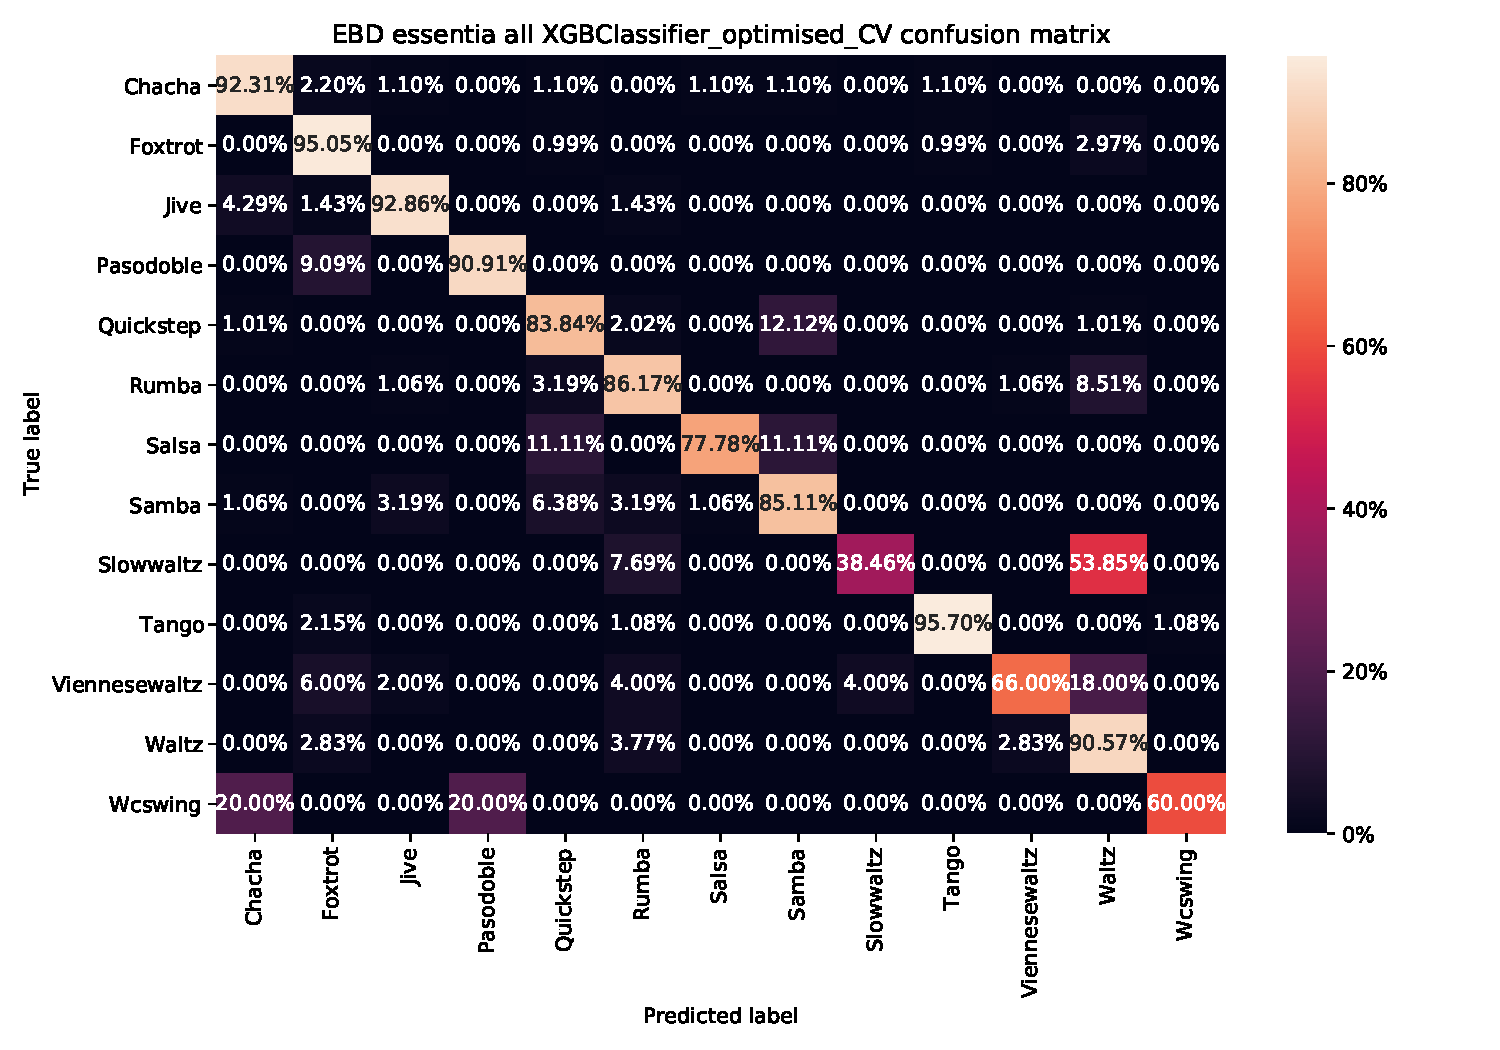
\includegraphics[width=\textwidth]{obrazky/EBD_essentia_all_XGBClassifier_optimised_CV_TS.pdf}
    \caption{\textbf{Matice predikcí nejúspěšnějšího klasifikátoru \textit{XGBClassifier} na datové sadě EBD.}}
    \label{obr_matice_predikce_EBD}
\end{figure*}

\begin{figure*}[h]
    \centering
    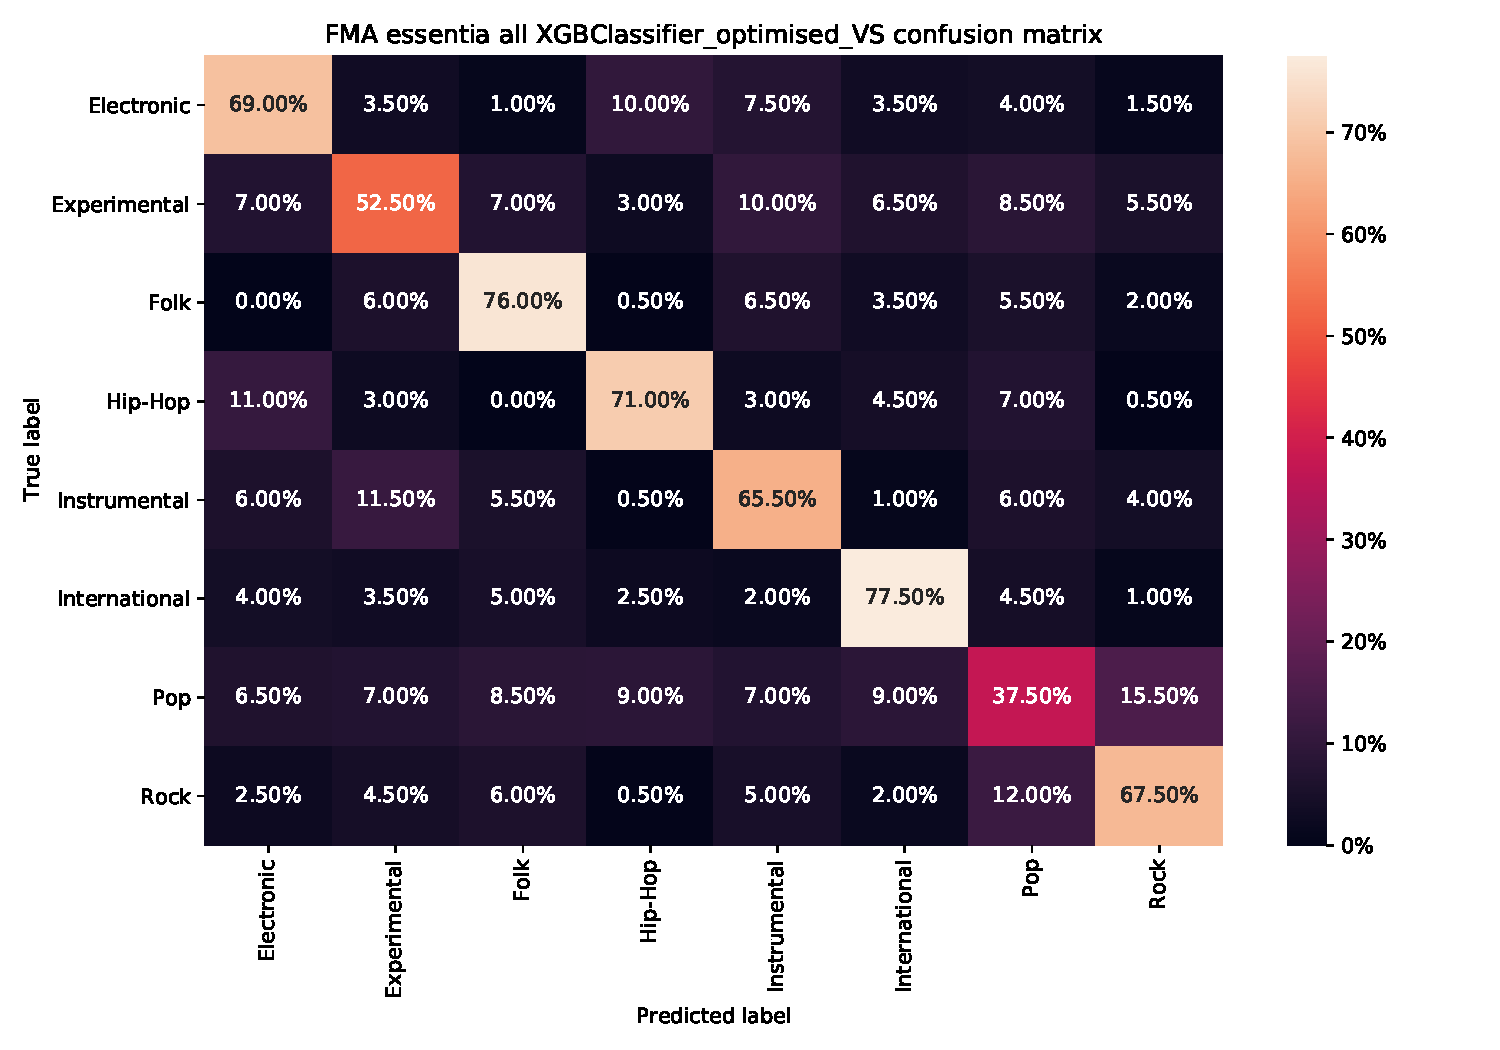
\includegraphics[width=\textwidth]{obrazky/FMA_essentia_all_XGBClassifier_optimised_VS_TS.pdf}
    \caption{\textbf{Matice predikcí nejúspěšnějšího klasifikátoru \textit{XGBClassifier} na datové sadě FMA.}}
    \label{obr_matice_predikce_FMA}
\end{figure*}

\begin{figure*}[h]
    \centering
    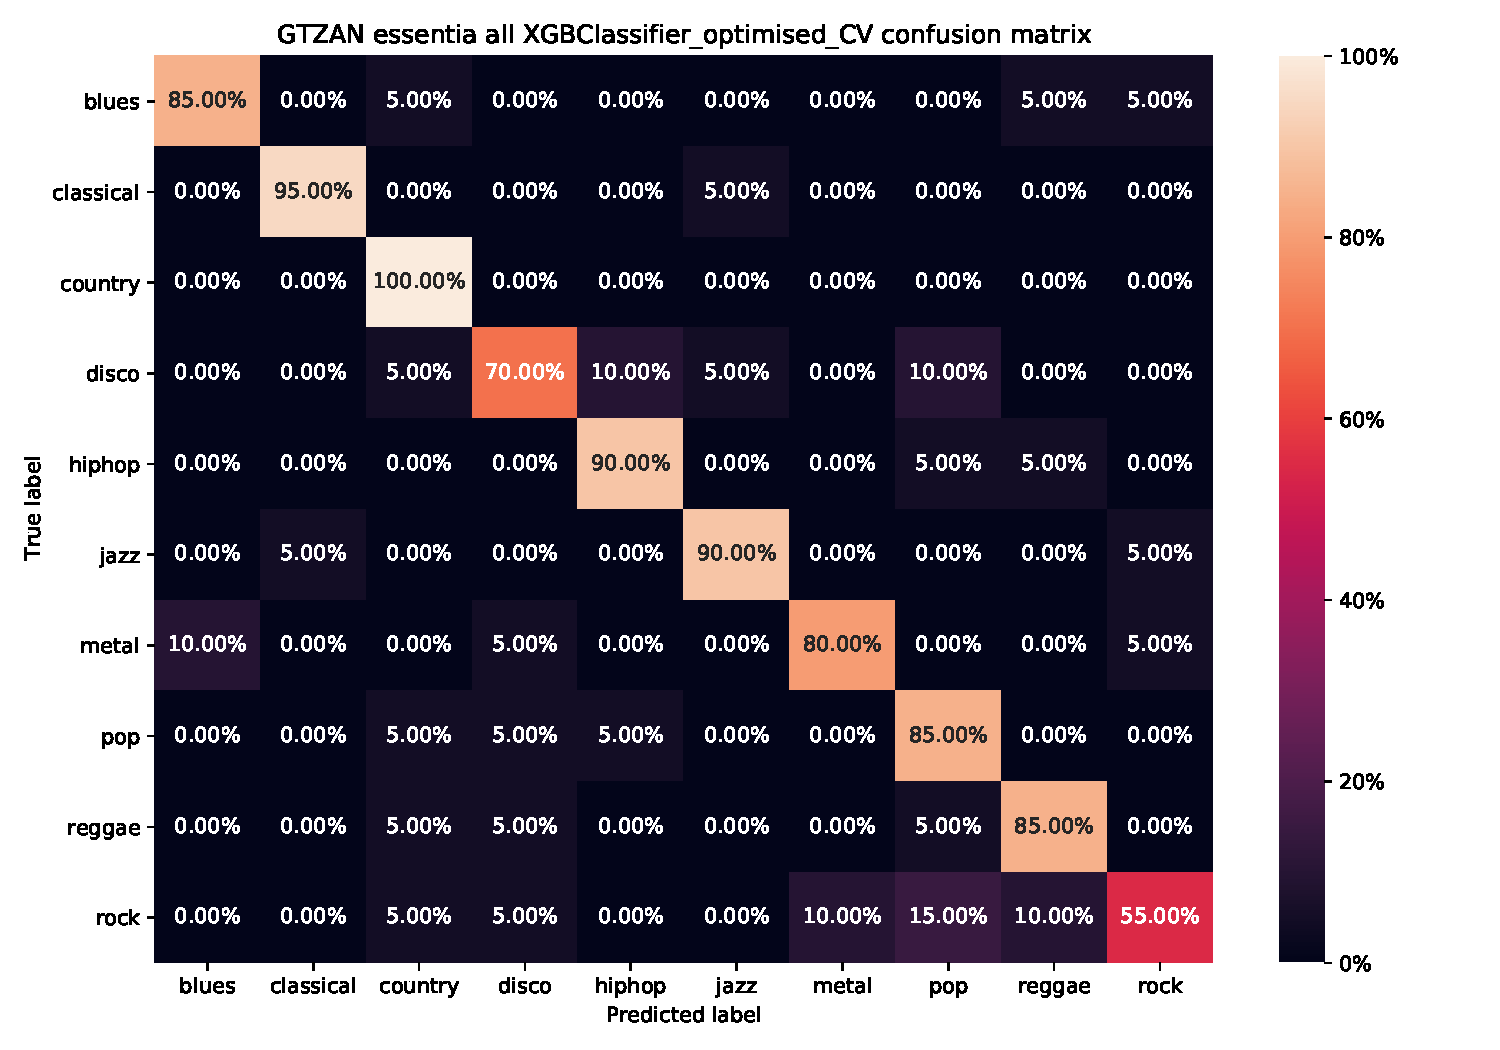
\includegraphics[width=\textwidth]{obrazky/GTZAN_essentia_all_XGBClassifier_optimised_CV_TS.pdf}
    \caption{\textbf{Matice predikcí nejúspěšnějšího klasifikátoru \textit{XGBClassifier} na datové sadě GTZAN.}}
    \label{obr_matice_predikce_GTZAN}
\end{figure*}

\chapter{Obsah přiloženého CD}
\label{obsah_prilozeneho_cd}

\dirtree{%
    .1 /\DTcomment{kořenový adresář přiloženého média}.
    .2 project\DTcomment{adresář obsahující soubory projektu}.
    .3 data\DTcomment{adrasář obsahující testovací skladby}.
    .4 local\_archive\DTcomment{adrasář reprezentující lokální hudební archiv}.
    .5 \dots.
    .3 metadata\DTcomment{adresář obsahující vygenerovaná data}.
    .4 misc\DTcomment{adresář obsahující ostatní soubory}.
    .5 columns\_fix.json\DTcomment{názvy sloupců atributů pro natrénované klasifikátory}.
    .5 feature\_extraction.out\DTcomment{výpis průběhu extrakce atributů}.
    .5 feature\_selection.out\DTcomment{výpis průběhu selekce atributů}.
    .5 optimised\_feature\_sets.json\DTcomment{vybrané podmnožiny atributů}.
    .5 optimised\_hyper\_parameters.json\DTcomment{optimalizované parametry}.
    .4 optuna\_studies\DTcomment{adresář obsahující soubory k~optimalizaci parametrů}.
    .5 EBD\_essentia\_all\_XGBClassifier\_CV.pkl.
    .5 FMA\_essentia\_all\_XGBClassifier\_VS.pkl.
    .5 GTZAN\_essentia\_all\_XGBClassifier\_CV.pkl.
    .4 test\_data\DTcomment{adresář obsahující testovací data}.
    .5 EBD\_genres.csv\DTcomment{žánry testovacích dat EBD}.
    .5 EBD\_X\_test.csv\DTcomment{atributy testovacích dat EBD}.
    .5 FMA\_genres.csv\DTcomment{žánry testovacích dat FMA}.
    .5 FMA\_X\_test.csv\DTcomment{atributy testovacích dat FMA}.
    .5 GTZAN\_genres.csv\DTcomment{žánry testovacích dat GTZAN}.
    .5 GTZAN\_X\_test.csv\DTcomment{atributy testovacích dat GTZAN}.
    .4 track\_genre\_lists\DTcomment{adresář se soubory s~informacemi o~žánrech skladeb}.
    .5 EBD\_track\_genre\_list.csv.
    .5 FMA\_track\_genre\_list.csv.
    .5 GTZAN\_track\_genre\_list.csv.
    .4 trained\_classifiers\DTcomment{adresář obsahující natrénované klasifikátory}.
    .5 EBD\_essentia\_all\_XGBClassifier\_optimised\_CV\_TS.joblib.dat.
    .5 FMA\_essentia\_all\_XGBClassifier\_optimised\_VS\_TS.joblib.dat.
    .5 GTZAN\_essentia\_all\_XGBClassifier\_optimised\_CV\_TS.joblib.dat.
    .3 src\DTcomment{adresář obsahující zdrojové soubory projektu}.
    .4 classification.ipynb\DTcomment{trénování a klasifikace}.
    .4 feature\_extraction.ipynb\DTcomment{extrakce atributů}.
    .4 feature\_selection.ipynb\DTcomment{selekce atributů}.
    .4 hpoptimise\_optuna.ipynb\DTcomment{třída s~funkcemi pro optimalizaci parametrů}.
    .4 images.ipynb\DTcomment{generace obrázků do technické zprávy}.
    .4 local\_archive\_predictions.ipynb\DTcomment{predikce a anotace lokálního archivu}.
    .4 misc.ipynb\DTcomment{funkce pro výpisy výsledků selekce/optimalizace/klasifikace}.
    .4 parameter\_tuning.ipynb\DTcomment{optimalizace parametrů}.
    .4 track\_genre\_list\_creation.ipynb\DTcomment{tvorba souborů s~informacemi o~žánrech}.
    .2 xslade21-latex\DTcomment{adresář obsahující soubory pro generaci technické zprávy}.
    .3 bib-styles\DTcomment{adresář obsahující styly pro latex}.
    .4 \dots.
    .3 obrazky\DTcomment{adresář obsahující obrázky technické zprávy}.
    .4 \dots.
    .3 template-fig\DTcomment{adresář obsahující loga fakulty}.
    .4 \dots.
    .3 fitthesis.cls\DTcomment{latex třída pro technickou zprávu}.
    .3 Makefile\DTcomment{makefile pro vytvoření technické zprávy}.
    .3 xslade21-Klasifikace-hudebnich-souboru.tex.
    .3 xslade21-Klasifikace-hudebnich-souboru-01-kapitoly-chapters.tex.
    .3 xslade21-Klasifikace-hudebnich-souboru-20-literatura-bibliography.bib.
    .3 xslade21-Klasifikace-hudebnich-souboru-30-prilohy-appendices.tex.
    .3 zadani.pdf\DTcomment{zadání projektu}.
    .2 install.sh\DTcomment{skript pro instalaci potřebných knihoven}.
    .2 makefile\DTcomment{makefile pro instalaci Python knihoven (pro install.sh)}.
    .2 Návod-k-instalaci-a-použití.txt\DTcomment{Návod k~instalaci a použití}.
    .2 requirements.txt\DTcomment{seznam potřebných knihoven (pro makefile)}.
    .2 Struktura-obsahu-média.pdf\DTcomment{soubor s~tímto obsahem}.
    .2 xslade21-Klasifikace-hudebnich-souboru.pdf\DTcomment{soubor s~technickou zprávou}.
}
  \fi
  
  % Kompilace po částech (viz výše, nutno odkomentovat)
  % Compilation piecewise (see above, it is necessary to uncomment it)
  %\subfile{xslade21-Klasifikace-hudebnich-souboru-30-prilohy-appendices}
  
\end{document}
